\chapter{Flood frequency analysis with a 200-year long stage series}
\label{chap:ch3}
%\markboth{Valorisation des données hydrométriques anciennes}{Valorisation des données hydrométriques anciennes}

\begin{figure}[h]
	\centering
		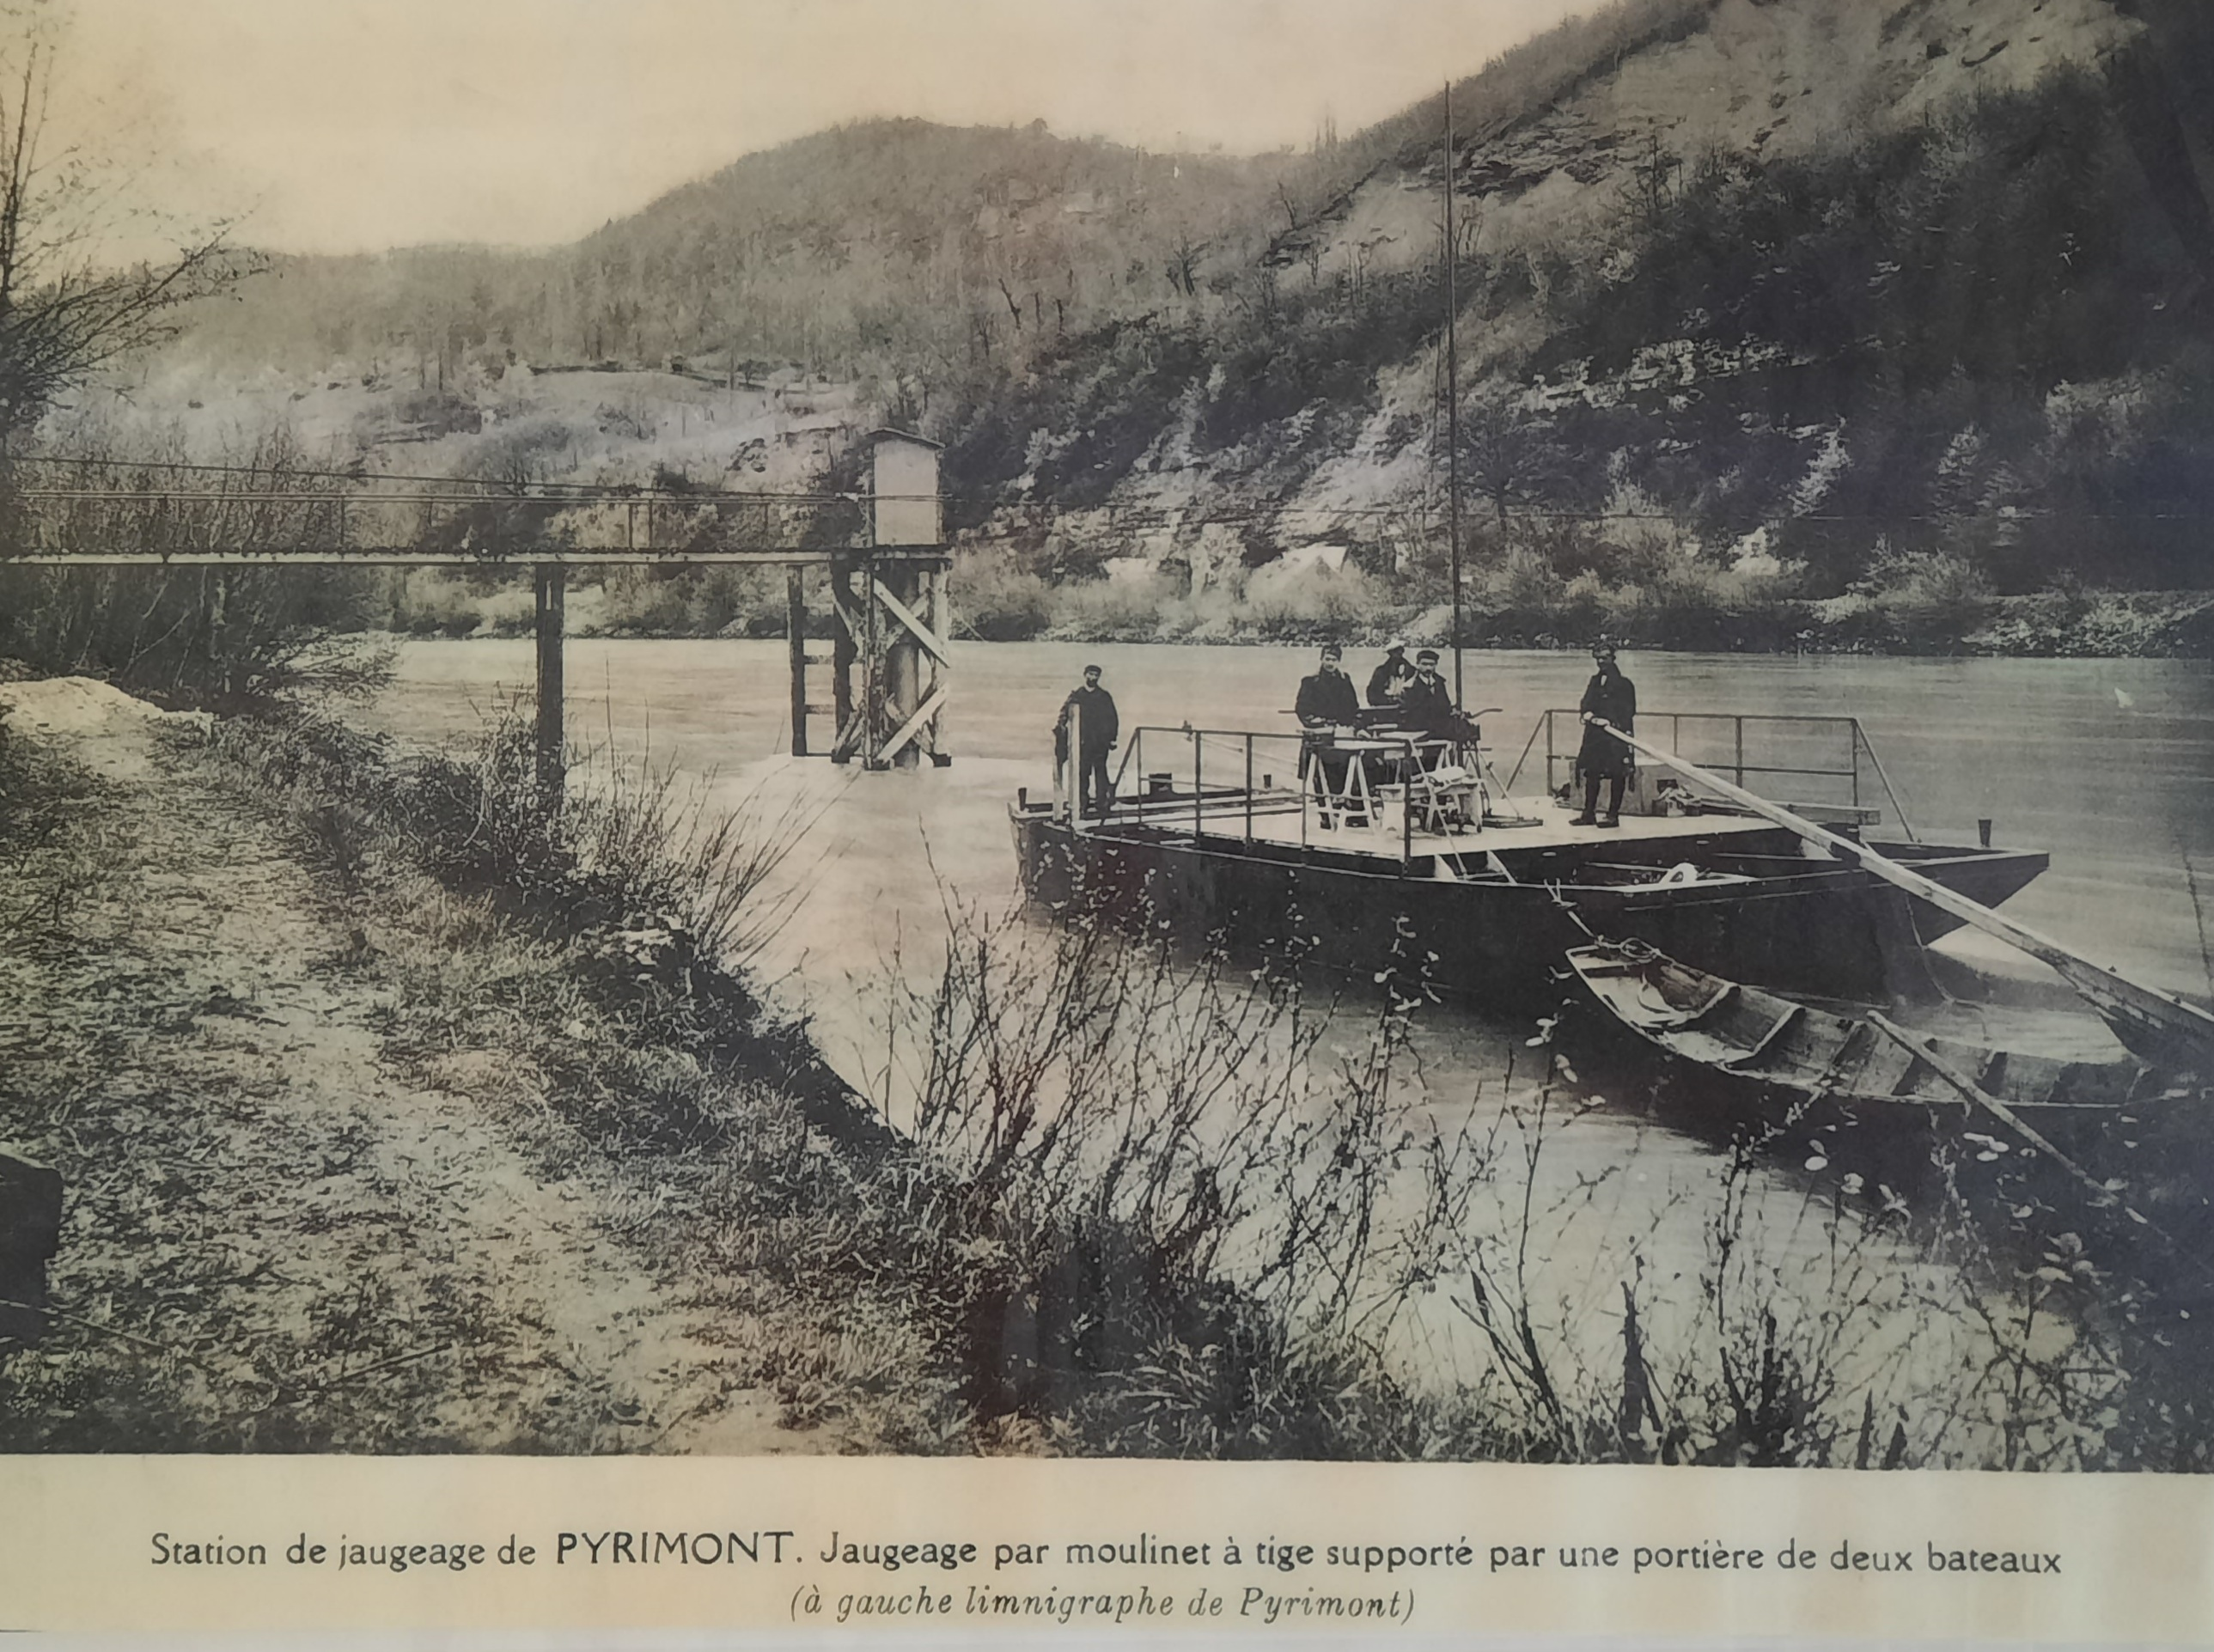
\includegraphics[width=.9\linewidth]{Chapitre3/Figures/Pyrimont.jpg}
        \caption{Jaugeage du Rhône à Pyrimont. Collection CNR}	
\end{figure}


\newpage
\FloatBarrier
\paragraph{} Ce chapitre est constitué d'un article scientifique publié dans la revue "Journal of Hydrology" et accepté le 16/06/2023.


\begin{figure}[h!]
    \centering
        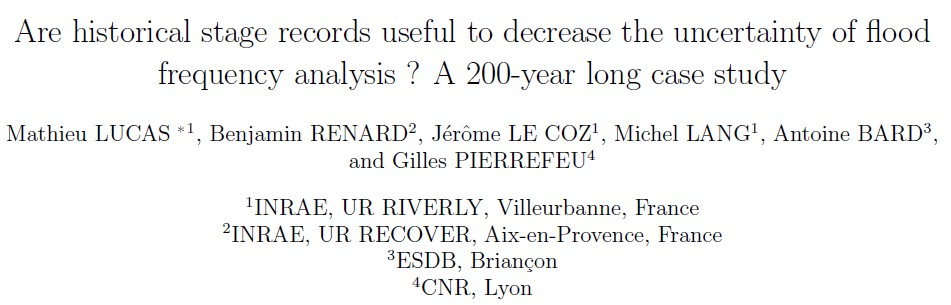
\includegraphics[width=\linewidth]{Chapitre3/Figures/Titre.jpg}
\end{figure}
\FloatBarrier

\section{Résumé}

L'analyse fréquentielle des crues est une méthode largement utilisée pour estimer le risque d'inondation. Elle est affectée par plusieurs sources d'incertitude. L'extension des chroniques de débit par l'utilisation de chroniques de hauteurs d'eau anciennes a le potentiel de réduire cette incertitude d'échantillonnage. Les débits anciens estimés sont généralement affectés par de grandes incertitudes. Cet article étudie l'intérêt de l'utilisation de chroniques de hauteurs d'eau anciennes pour améliorer les estimations des quantiles de crue extrêmes à travers une chaine de propagation diverses incertitudes. Les incertitudes sont estimées et propagées à partir des mesures limnimétriques et des courbes de tarages jusqu'aux quantiles de crue à l'aide de procédures Monte Carlo. La part des incertitudes hydrométriques et des incertitudes d'échantillonnage dans les estimations de quantiles de crue est examinée. Cette procédure est appliquée à la série journalière de hauteurs d'eau longue de 205 ans à la station hydrométrique du Rhône à Beaucaire, France (95 590 km\textsuperscript{2}). L'incertitude à 95\% des débits maximum annuels estimés varie de 30\% (XIX\textsuperscript{ème} siècle) à 5\% (1967-2020). L'incertitude totale des quantiles de crues est considérablement réduite lorsque la longueur de la série de débits utilisée passe de 20 à 100 ans en raison de la réduction de l'incertitude d'échantillonnage. Cependant, l'incertitude totale reste stable au-delà de cette taille d'échantillon : ceci est dû au fait que d'importantes incertitudes affectent les débits des crues du XIX\textsuperscript{ème} siècle, ce qui compense la réduction de l'incertitude d'échantillonnage. L'utilisation de la chronique totale longue de deux siècles conduit à inclure les deux plus fortes crues connues, en 1840 et 1856. Cela induit une augmentation de 15\% de l'estimation de la crue millénale, ce qui représente une augmentation mineure compte tenu des fortes incertitudes

\section{Abstract}
    
    Flood frequency analysis (FFA), a widely used method to estimate flood hazard, is affected by several sources of uncertainty. Extending flood samples by reanalyzing historical systematic stage records has the potential to reduce sampling uncertainty, but the historical flood discharges derived from this reanalysis are generally affected by large uncertainties. This paper explores whether historical stage records improve design flood estimates through a chain of uncertainty estimation methods for FFA. Uncertainties are estimated and propagated from stage and rating curves to design flood estimates using Monte Carlo procedures. The role of both streamflow and sampling uncertainties in design flood estimation is examined. This procedure  is applied to the 205-year long systematic stage series of the Rhône River at Beaucaire, France (95 590 km\textsuperscript{2}). The estimated streamflow 95\% uncertainty varies from 30\% (XIX\textsuperscript{th} Century) to 5\% (1967-2020). The total uncertainty of design flood is significantly reduced when the length of the series increases from 20 to 100 years due to sampling uncertainty reduction. However, the total uncertainty remains stable beyond this sample size: this is because large uncertainties affecting the XIX\textsuperscript{th} Century flood discharges compensate for the reduction in sampling uncertainty. Enlarging the sample size to two centuries leads to including the two largest known floods in 1840 and 1856. In turn, this induces a 15\% increase of the 1000-year flood estimates.
    \newline
    \textbf{Keywords}: Flood frequency analysis, Historical stage records, Uncertainty propagation, Streamflow uncertainty, Sampling uncertainty
        

\section{Introduction}
    \paragraph{}
    Flood frequency analysis (FFA) is a widely used method to estimate flood hazard. It allows linking the magnitude of a flood to its probability of occurrence (\citet{hamed_flood_2019}; \citet{jain_design_2019}). Flood estimates for various exceedance probabilities or, equivalently, return periods, are commonly used for population safety policies, land use planning, as well as industrial safety. The standard FFA approach is to estimate a distribution using a sample of flood peaks, typically defined as annual maximum discharges or discharges over a given threshold. This estimated distribution may be extrapolated to reach the desired flood quantile that typically corresponds to a 100 or 1000-year return period (see \cite{le_delliou_recommandations_2014} for dam safety regulations in France). 
    
    \paragraph{}
    This FFA approach is affected by various sources of uncertainty. First, the hydrological data used to estimate the FFA distribution is uncertain. Indeed, streamflow time series are generally derived from stage time series through rating curve models \citep{rantz_measurement_1982}. This procedure includes three types of errors on hydrological data: stage measurement; discharge measurement (gaugings); stage-discharge model (rating curve). Moreover, the estimated FFA distribution is also affected by sampling uncertainty resulting from the limited size of available streamflow data \citep{kjeldsen_uncertainty_2011}. Considering the importance of decisions relying on FFA results, a consistent treatment of uncertainty all over the data processing chain (including both streamflow and sampling uncertainties) is essential but is usually not performed.
    
    \paragraph{}
    Streamflow series are affected by several sources of uncertainty as described by \citet{mcmillan_benchmarking_2012}. First, a large number of stage error sources are identified in the literature (\citet{van_der_made_determination_1982}; \citet{petersen-overleir_uncertainty_2005}; \citet{mcmillan_benchmarking_2012}; \citet{horner_impact_2018}), such as staff gauge reading, levelling of the staff gauge, or stage sensor calibration. The frequency of measurement may also induce time interpolation errors. With modern automatic gauges, stage is generally measured with a time step small enough (e.g. between 15 min and 1 hour) to get negligible time interpolation errors. However, before the rise of automatic gauges, measurements were made by operators who read the staff gauge less frequently (e.g. once or a few times per day), thus possibly missing the flood peak. This issue is particularly critical when old stage series are used. \citet{hamilton_quantifying_2012} and \citet{kuentz_hydrometrie_2014} estimated the measurement frequency error by sub-sampling recent, sub-hourly measurements. They calculated the difference between the variable of interest (such as the daily maximum stage) derived from scarce data, and the same variable derived from high-frequency measurements. \citet{kuentz_hydrometrie_2014} applied the (monthly-averaged) calculated bias to correct old stage series. This correction aimed at taking into account the error due to the daily variability caused by snow melt. However, this type of correction has never been applied to peak stage correction during floods, especially in the case of long stage series.
    
    \paragraph{}
    Rating curve uncertainty is also a major issue when dealing with streamflow series. Transforming stage into discharge requires calibration data (gaugings) to establish the stage-discharge relationship. Note that the term "gauging" corresponds in this paper (and in the French practice) to the sporadic measurement of the stage-discharge couple, which can correspond to the term "discharge measurement" in the British or American practice. Gaugings uncertainty depends on the measurement method (\citet{lecoz_quantification_2014}; \citet{puechberty_charte_2017}). Moreover, the rating curve is also affected by uncertainties coming from the imperfection of the chosen model to represent the actual hydraulic configuration, and from parameter estimation. Many methods have been proposed to quantify these uncertainties (\citet{petersen-overleir_bayesian_2009}; \citet{juston_rating_2014}; \citet{le_coz_combining_2014}; \citet{morlot_dynamic_2014}; \citet{coxon_novel_2015}; \citet{mcmillan_rating_2015}; \citet{mansanarez_rapid_2019}). A comparison of several of these methods has been recently proposed by \citet{kiang_comparison_2018}. Another important issue affecting streamflow data accuracy is rating changes. The stage-discharge relationship is frequently affected by changes caused by various factors, either natural or anthropic, for instance: bed geometry evolution during floods or river works, aquatic vegetation growth and decay, ice cover... A regular monitoring through gaugings is essential to detect those changes \citep{ibbitt_gauging_1987} that can be transient or sudden. Several methods have been proposed to deal with rating changes: estimating rating curves on moving temporal windows (\citet{westerberg_stage-discharge_2011}; \citet{guerrero_temporal_2012}), computing as many rating curves as there are gaugings \citep{morlot_dynamic_2014}, exploring changes in the annual minimum stages \citep{lapuszek_methods_2015}, selecting the 0.5-year return period discharge as a threshold for rating changes \citep{mcmillan_impacts_2010}. More recently, \citet{darienzo_detection_2021} proposed a method based on a recursive segmentation procedure, accounting for both gaugings and rating curve uncertainties. This method has a particular interest when dealing with old and uncertain gaugings. Following the detection of rating shifts, rating curves should be estimated for each stable period. This task may not be straightforward, as the number of gaugings available within a stable period is not always sufficient to properly estimate the stage-discharge relationship for the whole discharge range. A common way to address the lack of gaugings (in particular flood gaugings) within some of the stable periods is to use gaugings from the other stable periods (\cite{mcmillan_benchmarking_2012}; \cite{puechberty_charte_2017}). \citet{mansanarez_shift_2019} proposed an alternative approach to deal with this issue. They developed a stage-period-discharge (SPD) model where rating curve parameters may vary across periods, while others are supposed constant. This method has the advantage of transferring information between periods to improve the rating curve estimation, even when few gaugings are available.
    
    \paragraph{}
    Estimating sampling uncertainty in FFA is a well-established approach. Whatever the chosen distribution and estimation method, standard statistical procedures are available \citep{coles_classical_2001}. However, these standard procedures only quantify sampling uncertainty, they do not consider data uncertainty. The literature review proposed in the previous paragraphs shows that methods for quantifying individual sources of uncertainty (stage, rating curve and FFA distribution estimation) are available. However, the way these multiple uncertainties propagate through the FFA analysis chain has been less thoroughly studied. A few solutions have emerged to propagate uncertainties in stage time series through uncertain rating curves (\citet{dymond_accuracy_1982}; \citet{herschy_hydrometry_1998}; \citet{petersen-overleir_uncertainty_2005}), but they assume independent stage errors and therefore neglect systematic errors. \citet{horner_impact_2018} proposed a method for the propagation of both sources of stage uncertainty through uncertain rating curves. Therefore, it is possible to distinguish the effects of independent and systematic stage errors on streamflow uncertainty. \citet{petersen-overleir_accounting_2009}, \citet{steinbakk_propagation_2016}, and \citet{vieira_assessing_2022} performed an integrated analysis in which both rating curve parameters and flood frequency distribution are estimated. These studies highlighted the importance of considering rating curve uncertainty for design flood estimations and concluded that, under some conditions, accounting for rating curve uncertainty may notably widen the uncertainty intervals around flood quantiles. However, these studies did not consider stage measurement and time interpolation errors nor rating changes, which may constitute a major source of uncertainty for streamflow data. This is particularly the case when dealing with long streamflow series for which stage uncertainty is large and variable through time, and rating changes may have been missed. Their consideration of all these sources of uncertainty is necessary.
        
    \paragraph{}
    The following questions will be considered in this paper: 
    \begin{itemize}
        \item[1.] How to make the most of historical hydrometric (based on stage records) data in flood frequency analysis while accounting for multiple and variable uncertainties at each step of the procedure ? 
        
        \item[2.] What is the contribution of each source of uncertainty to the flood quantile uncertainty when historical data are taken into account ? 
        
        \item[3.] To what extent does enlarging streamflow samples by adding increasingly uncertain historical data improve flood quantiles estimation ? How are the relative contributions of sampling and streamflow uncertainties evolving with sample size ?
    \end{itemize}

    \paragraph{}
    Note that the "historical data" term used in this paper refers to the use of old but continuously measured stage series, as opposed to sporadic flood marks, prior to regular stage measurements. 

    \paragraph{}
    This paper illustrates the chained application of methods to quantify and propagate uncertainty from stage records (and their limited time resolution) and stage-discharge rating curves to the estimation of flood distribution with uncertainties. While most of these methods already exist, a key novelty of this work is their combination in a consistent framework (Figure \ref{fig:ChProp}) to provide an end-to-end evaluation of the  uncertainty affecting FFA estimates. An original method to quantify the stage uncertainty stemming from infrequent readings is also proposed.

    The paper is organized as follows. First, the methodology for establishing uncertain streamflow series in a century-long context is presented. It goes through the detection of rating shifts (section \ref{subsec:RatingShifts}), the estimation of rating curves (section \ref{subsec:RC_SPD}), and the estimation (section \ref{subsec:StageErr}) and propagation (section \ref{subsec:PropagStage}) of stage errors. Then, an approach to propagate streamflow uncertainty through the estimation of extreme flood quantiles is proposed (section \ref{subsec:FFA}). This procedure is applied to the Beaucaire gauge on the Rhône River (section \ref{sec:Bcr}), which previous official FFA only used a 80-year long discharge series \citep{rigaudiere_etude_2000}. In France, the official design flood for flood risk mapping is based on the “largest known flood” or the Q100 flood (AEP=0.01) if the latter is greater. Uncertainty is not taken into account in the official rules. The recent works of \citet{pichard_hydro-climatology_2017} and \citet{bard_actualisation_2018} provided a systematic stage series from 1816 to the present time, which makes it the ideal case study for demonstrating this procedure. The results of this application are presented in section \ref{sec:Results}, and they are discussed in section \ref{sec:Discussion}, where avenues for improvements are proposed.
    
    \begin{figure}[h!]
    \centering
        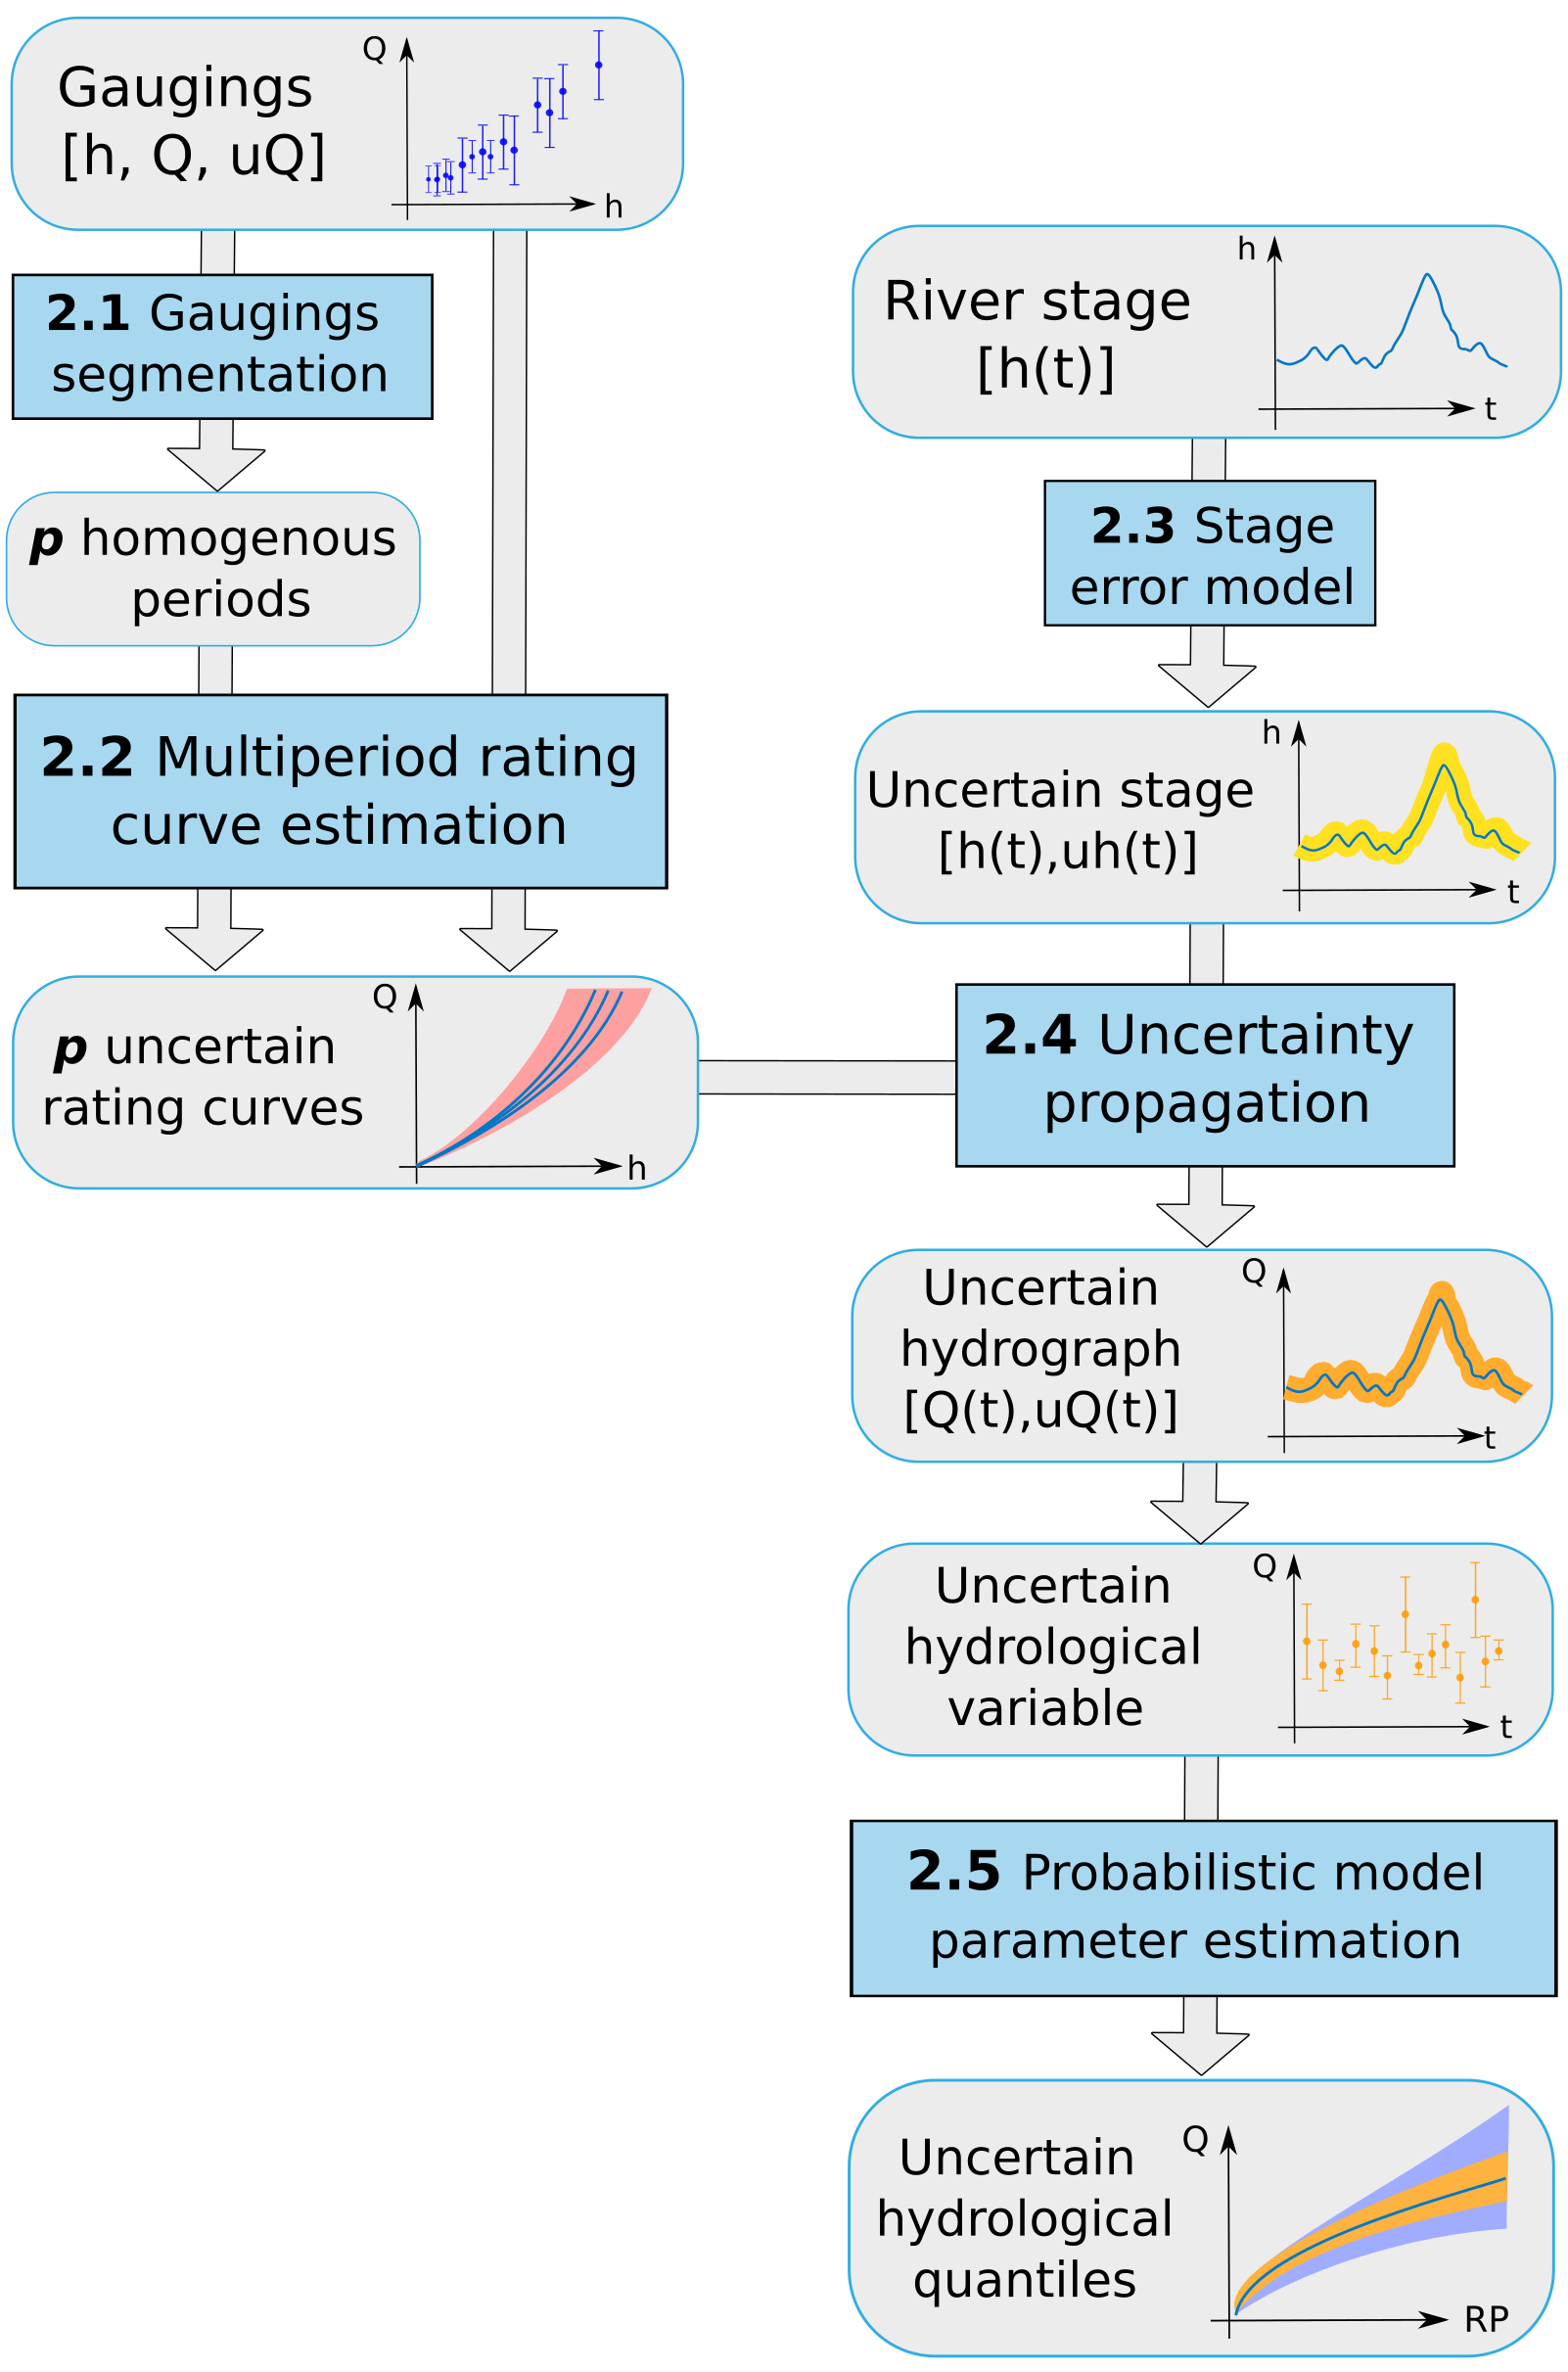
\includegraphics[width = 8cm]{Chapitre3/Figures/1-uTotSchema.png}
        \caption{Block diagram of the uncertainty propagation procedure. Grey blocks represent data, blue blocks stand for analysis methods/models that correspond to the sub-sections of this article. $h$ is the water stage, $uh$ the stage uncertainty, $Q$ the discharge, $uQ$ the discharge uncertainty, $t$ is the time and $RP$ the return period of flood quantiles.}
        \label{fig:ChProp}
    \end{figure}
    \FloatBarrier
    
\section{Uncertainty propagation chain for flood frequency analysis}
     \subsection{Rating shifts detection}
     \label{subsec:RatingShifts}
    
    The stage-discharge relationship is sensitive to sudden changes caused by morphogenic floods or other causes affecting the flow characteristics. Relying on residuals between the gaugings and the rating curve is the most common approach to monitor the stability of this relationship over time. The method proposed by \citet{darienzo_detection_2021} is used in this work and can be summarized as follows. First, a baseline rating curve is estimated from the whole gaugings dataset. The residuals between gaugings and the rating curve are determined, and a statistical segmentation procedure is applied to them. This procedure accounts for the residuals uncertainty, coming from both the gaugings uncertainty and the rating curve uncertainty. The optimal number of stable sub-periods is determined based on the Bayesian Information criterion (BIC). Then, the same steps are applied recursively to each sub-period. The recursive procedure is stopped when the BIC indicates that a single period is optimal for all sub-periods. The results are not only the dates of the rating shifts but the posterior probability density functions (pdf) of change point times. This allows affecting the shift time to the time of the maximum stage included in the posterior 95\% credibility interval. Prior knowledge is provided on the mean of the residuals in each sub-period. The maximum number of segments at each iteration also needs to be specified. All technical details can be found in \citet{darienzo_detection_2021}.
    
    \subsection{Multi-period rating curves estimation: stage-period-discharge model}
    \label{subsec:RC_SPD}
    \paragraph{}
    Once the stable periods have been identified, the next step is to estimate the rating curves. \citet{mansanarez_shift_2019} developed a stage-period-discharge (SPD) model "based on the physical interpretation of changes in the stage-discharge relation across a series of stability periods". The SPD model is based on the BaRatin model \citep{le_coz_combining_2014}.
    \paragraph{} BaRatin uses the Bayesian paradigm to estimate the parameters of the rating curve equation, a combination of power equations: $Q = a(h-b)^c$, where $Q$ is the discharge, $h$ is the stage, $b$ is an offset (corresponding to the cease-to-flow stage), and $a$ and $c$ are the coefficient and the exponent of the power function. The rating curve equation is deduced from a hydraulic analysis of the gauging station, aimed at identifying the main hydraulic controls governing the stage-discharge relation. The multiple controls can be activated successively or simultaneously. Bayesian inference allows deriving the posterior distribution of rating curve parameters by combining hydraulic information (priors for parameters of each hydraulic control) and information from gaugings with uncertainty (likelihood). Two sources of uncertainty are associated with the estimated rating curve. Parametric uncertainty reflects the uncertainty due to the rating curve parameters estimation because of the limited amount of gaugings and the gaugings uncertainty. Remnant uncertainty comes from the imperfection of the chosen rating curve model to represent the actual hydraulic configuration. The posterior distribution is explored using a Markov Chain Monte Carlo (MCMC) sampler, leading to $m$ realizations of the rating curve parameter vector representing parametric uncertainty. We refer the reader to \citet{le_coz_combining_2014} for a more thorough description.

    \paragraph{}
    The SPD model estimates the rating curves of each stable period based on the same principle by considering that some parameters vary in time, while others remain constant throughout the stable periods. An important step is the identification of those varying parameters based on an hydraulic analysis of the site. Generally, channel depths and/or widths are suspected to change. A distinction is made between "local changes" affecting the lowest control only (for instance the movement of the controlling riffle) and "overall changes" affecting several controls at the same time (for instance, the scouring or filling of the main channel, affecting the offsets of both the low-flow controlling riffle and the main channel itself). Prior specification for varying parameters can be based on the analysis of the yearly lowest stages, which provide information on the evolution of riverbed elevation, as described by \citet{lapuszek_methods_2015}. See \citet{mansanarez_shift_2019} for a detailed description of prior specification for time-varying rating curves. Specific investigation is needed to correctly account for past flood surveys of the cross section, as complex filling/erosion process may have been encountered during a flood with morphogenic changes.
    
    \subsection{Stage uncertainties}
    \label{subsec:StageErr}
    
    Many sources of error having distinct statistical properties can affect stage measurements, as described in \citet{horner_impact_2018}. Five different sources of error ($\delta_{1,...,5}$) affecting stage measurements are considered. Let $h(t)$ be the measured maximum stage of a day $t$. The unknown true maximum stage $\hbar(t)$ is assumed to be approximated by the following equation:
    
    \begin{equation}
        \hbar(t) = h(t) + \delta_1(t) + \delta_2(t) + \delta_3(t) + \delta_4(t) + \delta_5(t)
        \label{eq:StageError}
    \end{equation}

    \paragraph{}Staff gauge reading errors $\delta_1 \sim \mathcal{N}(0,\sigma_1)$ originate from operators reading the gauge, where $\sigma_1$ depends on the resolution of the graduations (usually 1 cm), and can be increased by waves, especially during floods \citep{mcmillan_benchmarking_2012}.

    \paragraph{}Nowadays, most stage measurements are done with automatic sensors of various types such as pressure sensors, floats, radars, and they require a calibration to link the water stage to the measured proxy (respectively the pressure of the water column, the height of a float, or the air draught). Two types of errors arise from this process: sensor errors $\delta_2 \sim \mathcal{N}(0,\sigma_2)$, where $\sigma_2$ is usually estimated by the sensor manufacturer, and sensor calibration errors $\delta_3 \sim \mathcal{N}(0,\sigma_3)$ that are related to the corrections made by operators when comparing the stage measured by the sensor to the actual stage at the staff gauge reference. An operator error at this step could affect the stage measurement until the next calibration. Sensor calibration error $\delta_3$ is hence assumed constant between two calibrations and can be represented by drawing a new random value at each operator intervention.
    
    \paragraph{}Datum errors $\delta_4  \sim \mathcal{N}(0,\sigma_4)$ are related to changes in the datum reference elevation of the staff gauge zero value and possible discontinuity between successive gauges. Similarly to $\delta_3$, this error is constant between two gauge changes or datum reference measurements. 
    
    \paragraph{}Measurement frequency errors $\delta_5$ are related to the inadequacy of the frequency of measurement with respect to the rate of stage variations, leading to the true daily maximum occurring in between measurements. Unlike other types of stage errors, this error is hence necessarily positive, which calls for using a positive distribution such as the Exponential distribution. The parameters of this distribution can be estimated with data from the recent period, by analyzing the difference between the daily maximum stage derived from the high-frequency sensor measurement and that from an infrequent fixed-time reading. Note that the frequency errors for hourly (or more frequent) measurements are considered negligible for large rivers with slow variations, such as the Rhône River at Beaucaire.
      
    \paragraph{}
    To sum up, $\delta_1$, $\delta_2$ and $\delta_5$ errors are drawn at each measurement time step, while $\delta_3$ and $\delta_4$ errors are only drawn at specific calibration times. Errors $\delta_1$ to $\delta_4$ are assumed Gaussian with known standard deviations, while $\delta_5$ is assumed Exponential with parameter estimated by subsampling recent measurements. For each error type, 500 realizations are drawn from their respective distribution. Applying eq. \ref{eq:StageError}, the total stage uncertainty is therefore represented by 500 possible realizations of the stage $\hbar(t)$.
   
   \subsection{Propagation of stage and rating curve uncertainties to streamflow time series}
   \label{subsec:PropagStage}
   Stage realizations can be propagated through uncertain rating curves, following the approach described by \citet{horner_impact_2018}. Four cases are considered to estimate the contributions of the different sources of streamflow uncertainty:
   
   \begin{itemize}
       \item \textbf{Case 1: Maxpost streamflow.} Stage is taken as the median of the stage time series realizations. This unique stage time series is propagated through the maxpost (Maximum A Posteriori: obtained with parameters maximizing the posterior pdf) rating curve, resulting in a single discharge time series. 
       
       \item \textbf{Case 2: Stage uncertainty.} The $n$=500 possible stage time series are propagated through the maxpost rating curve. Thus, $n$ discharge time series are obtained.
       
       \item \textbf{Case 3: Stage and parametric rating curve uncertainty.} The $n$=500 realizations of stage time series are propagated through $m$ rating curves, corresponding to the $m$ MCMC-simulated parameter vectors described in section \ref{subsec:RC_SPD}. This leads to $n \times m$ discharge time series. 
       
       \item \textbf{Case 4: Total streamflow uncertainty.} It is obtained by adding remnant rating curve uncertainty (as defined in section \ref{subsec:RC_SPD}) to case 3. To achieve this, $n \times m$ time series of remnant errors are sampled from their estimated distribution and added to the time series created for case 3. 
   \end{itemize}
   
    \subsection{Estimation of probabilistic model parameters and flood frequency analysis}
    \label{subsec:FFA}
    
    The Generalized Extreme Value (GEV) distribution is commonly used to model annual maximum discharges (AMAX) (see \citet{hamed_flood_2019} or \citet{jain_design_2019}). The vector $\boldsymbol{\theta} = (\mu,\sigma,\xi)$ denotes the location, scale and shape parameters of the GEV distribution. The parameters can be estimated based on an independent and identically distributed ($iid$) sample of $j$ annual maximum discharges $(q_t)_{t=1,...,j}$. Bayesian-MCMC estimation is used in this work, as described in \citet{coles_classical_2001}. The posterior distribution quantifies sampling uncertainty and can be represented by $r$ MCMC-generated GEV parameter vectors $\boldsymbol{\Theta} = (\boldsymbol{\theta}_1,...,\boldsymbol{\theta}_r)$. The maxpost vector is noted $\boldsymbol{\hat{\theta}}$.
    
    \paragraph{}
    As described in section \ref{subsec:PropagStage}, total streamflow uncertainty is represented by $n \times m$ possible realizations of the streamflow, hence of the AMAX series $(q_t^{(i)})_{i=1,...,n \times m;\;t=1,...,j}$, that are subsampled to $s$=500 realizations to reduce computation time. The estimated flood quantiles should consider both sampling and streamflow uncertainties. Similarly to \citet{steinbakk_propagation_2016}, the aim is to estimate the contribution of each source to the total uncertainty. For this purpose, three cases can be considered:
    
    \begin{itemize}
        % MP: median of stage err x maxpost RC x maxpost GEV
        \item \textbf{Case 1: Maxpost quantiles.}        
        The GEV distribution is estimated using the  single AMAX series $\mathbf{\hat{q}} = (\hat{q_t})_{t=1,...,j}$ derived from the maxpost streamflow series (case 1 in section \ref{subsec:PropagStage}). Flood quantiles are then computed using the maxpost GEV parameters $\boldsymbol{\hat{\theta}} =  (\hat{\mu}, \hat{\sigma}, \hat{\xi})$. In this case, both streamflow and sampling uncertainties are ignored.
        
        % Hydro U: hydrometric U realizations x maxpost GEV
        \item \textbf{Case 2: Streamflow uncertainty}. The GEV distribution is estimated for each possible AMAX realization: $\mathbf{q}^{(i)} = (q_t^{(i)})_{t=1,...,j;\;i=1,...,s}$. However, only the maxpost GEV parameters vector is retained for each realization. This results in $s$ vectors of GEV parameters $(\boldsymbol{\hat{\theta}}^{(i)})_{i=1,...,s}$ that represent the effect of streamflow uncertainty of flood quantiles, ignoring sampling uncertainty.
    
        % Total U
        \item \textbf{Case 3: Total uncertainty.} Similarly to Case 2, the GEV distribution is estimated for each of the $s$ realizations of the AMAX series, but all the $r$ MCMC-simulated GEV parameters are used, leading to $s \times r$ vectors of GEV parameters $(\boldsymbol{\theta}^{(i)}_k)_{k=1,...,r;\;i=1,...,s}$. The result thus reflects both sampling and streamflow uncertainties.
    \end{itemize}
    
\section{Case study: The Rhône River at Beaucaire}
\label{sec:Bcr}
    \subsection{Site}
    
    The Rhône River at Beaucaire (95 590 km\textsuperscript{2}) is the lowest gauge of the Rhône River (Figure \ref{fig:locstations}). It captures all the complexity of the Rhône River hydrological regime, from the Alpine area to the oceanic and Mediterranean influences. The annual mean discharge is around 1700 m\textsuperscript{3}/s \citep{bard_actualisation_2018}, and the maximum known discharge reached 12 500 $m^3/s$ (May 1856, \citet{lang_les_2014}). The station lies in a flood sensitive area, as illustrated by the recent 2003 flood, resulting in 1.1 billion euros worth of damage \citep{lang_les_2014}. 
    The first stage measurements started in 1816, close to the bridge linking the cities of Beaucaire and Tarascon. This station is named "Pont de Beaucaire" (Kilometric point 267.6 from Lyon). It has been used until the construction of the Vallabrègues hydroelectric scheme in 1967, which led to the derivation of a part of the discharge. Consequently, a new gauging station was installed 2~km downstream from the original one, downstream from the restitution of the derivated discharges. This station, logically named "Beaucaire Restitution" (Kilometric point 269.5), has been used ever since. This resulted in a data gap during the construction process between 1967 and 1970.

    \begin{figure}[h!]
        \centering
        \includegraphics[width = 11cm]{Chapitre3/Figures/2-BcrBv.png}
        \caption{The French Rhône River catchment and Beaucaire gauging stations (from www.geoportail.gouv.fr and www.openstreetmap.org)}
        \label{fig:locstations}
    \end{figure}
    % \FloatBarrier
 
    \subsection{Rating curves}
    \label{sec:prior_elicitation}
       
	\paragraph{} Many gauges of the Rhône River are subject to the effect of variable backwaters caused by the proximity of a dam, and therefore require the use of a stage-fall-discharge (SFD) rating curve model (for example, Valence gauge, 140 km upstream from Beaucaire described by \cite{mansanarez_non-unique_2016}). Beaucaire is located within a narrowing of the floodplain and there is no dam downstream from the gauge. However, a backwater effect from the sea has been observed at Beaucaire Restitution, but it only affects the very low flows. As this article focuses on floods, we assume that there is no reason to use a SFD model here. Consequently, like the gauge operator (CNR), a stage-discharge (SD) model is used for both Pont de Beaucaire and Beaucaire Restitution gauges.
                
        \subsubsection{Pont de Beaucaire}
        
         At Pont de Beaucaire, the stage-discharge relationship can be approximated by two additive channel controls: a main channel and a floodway. Thus, the rating curve equation can be written as follows: 

        \begin{equation}
        Q(h) =
          \begin{cases}
           a_1(h-b_1)^{c_1}, & \text{if $\kappa_1 < h \leq \kappa_2$ (main channel) }\\
           a_1(h-b_1)^{c_1}+ a_2(h-b_2)^{c_2}, & \text{if $h > \kappa_2$ (main channel + floodway)}
          \end{cases}
          \label{eq:RcPt}
        \end{equation}

    Within the main channel (when water stage is below $\kappa_2 \approx$ 2~m), the flow is splitted in two sub-channels (figure \ref{subfig:matrixCh}) since time immemorial (at least before 1816) as described by \citet{armand_ii_1907}. The mobile sandbars separating the flow were progressively fixed by dikes during the XIX\textsuperscript{th} Century to ease the navigation (figure \ref{subfig:diguesarmand}). These sub-channels are connected upstream and downstream from the gauge location, thus they can be modelled as a single main channel whose average width ($\approx$ 300~m) is the sum of the two sub-channels widths (figure \ref{subfig:matrixCh}). When stage exceeds $\kappa_2$, water starts flowing on the sandbars between the two subchannels. At the gauge location, the total width is limited by unsubmersible levees, but a floodway is also activated a few hundred meters downstream from the station, impacting the stage-discharge relationship at the gauge. The width of this floodway is around 500~m.   
    \paragraph{}
    The prior distributions of the rating curve parameters are specified using historical material retrieved in regional archives, as described in table \ref{tab:PriorPt}. Physical parameters that have a direct hydraulic meaning are expressed in the first three lines: channel width ($B$), slope ($S$) and Strickler coefficient ($K$). The resulting prior distribution for the inferred parameter $a=KB\sqrt S$ is deduced by Monte Carlo propagation. Log-normal priors are used for positive quantities such as slopes, channel widths and Strickler coefficients. Informative but imprecise priors are assigned to parameters such as channel widths, slopes or offsets which can be difficult to estimate precisely. For $c$ exponents, very precise priors are used because they depend on the control type and shape (here $c=5/3$ for wide rectangular channel controls based on the simplified Manning-Strickler equation as described by \citet{le_coz_combining_2014}). Structural uncertainty parameters have uninformative priors.
    \paragraph{}
    According to historical profiles and cross-sections, we assume that changes affecting main channel and floodway controls may have occurred due to major floods (in particular 1840, 1856 and 1935 floods) and that channel widths remained constant. Those changes are called "overall changes" and are supposed to affect both main channel and floodway offsets ($b_1$ and $b_2$) at the same time.
    Meanwhile, we assume that local changes due to dike works or sediment depositions from small floods affected the offset ($b_1$) of the main channel only. As described by \citet{mansanarez_shift_2019}, local and overall changes $\Delta_l^{(k)}$ and $\Delta_g^{(k)}$ affect the offsets of two consecutive periods ($(k-1)$ and $k$) as follows: 
       
       \begin{equation}
          \begin{cases}
           b_1^{(k)} = b_1^{(k-1)}-(\Delta_g^{(k)}+\Delta_l^{(k)}), & \text{(incremental changes in the main channel)}\\
           b_2^{(k)} = b_2^{(k-1)}-\Delta_g^{(k)}, & \text{(incremental changes in the floodway)}
          \end{cases}
          \label{eq:SPD_Pt}
        \end{equation}
       
       As the most recent period obtained by gaugings segmentation is assumed to be the most accurately known, it is used as the reference period ($k=1$) and periods are numbered backward in time. Prior distributions of offset changes are determined in section \ref{sec:stageevolution}.       

        \begin{figure}[h!]
            \centering
            \begin{subfigure}{0.7\linewidth}
            \centering
            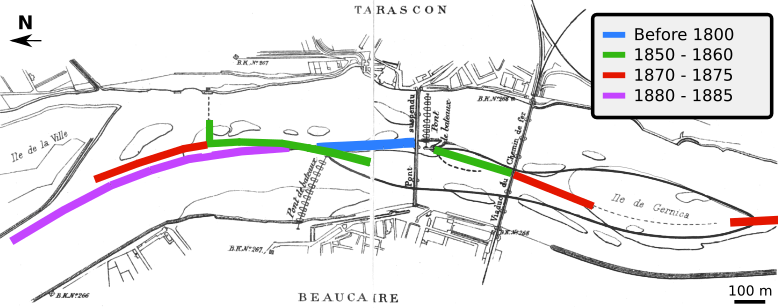
\includegraphics[width=1\linewidth]{Chapitre3/Figures/3a-DiguesArmand.png}\hfill
            \caption{}
            \label{subfig:diguesarmand}
            \end{subfigure}
            
            \begin{subfigure}{0.6\linewidth}
            \centering
            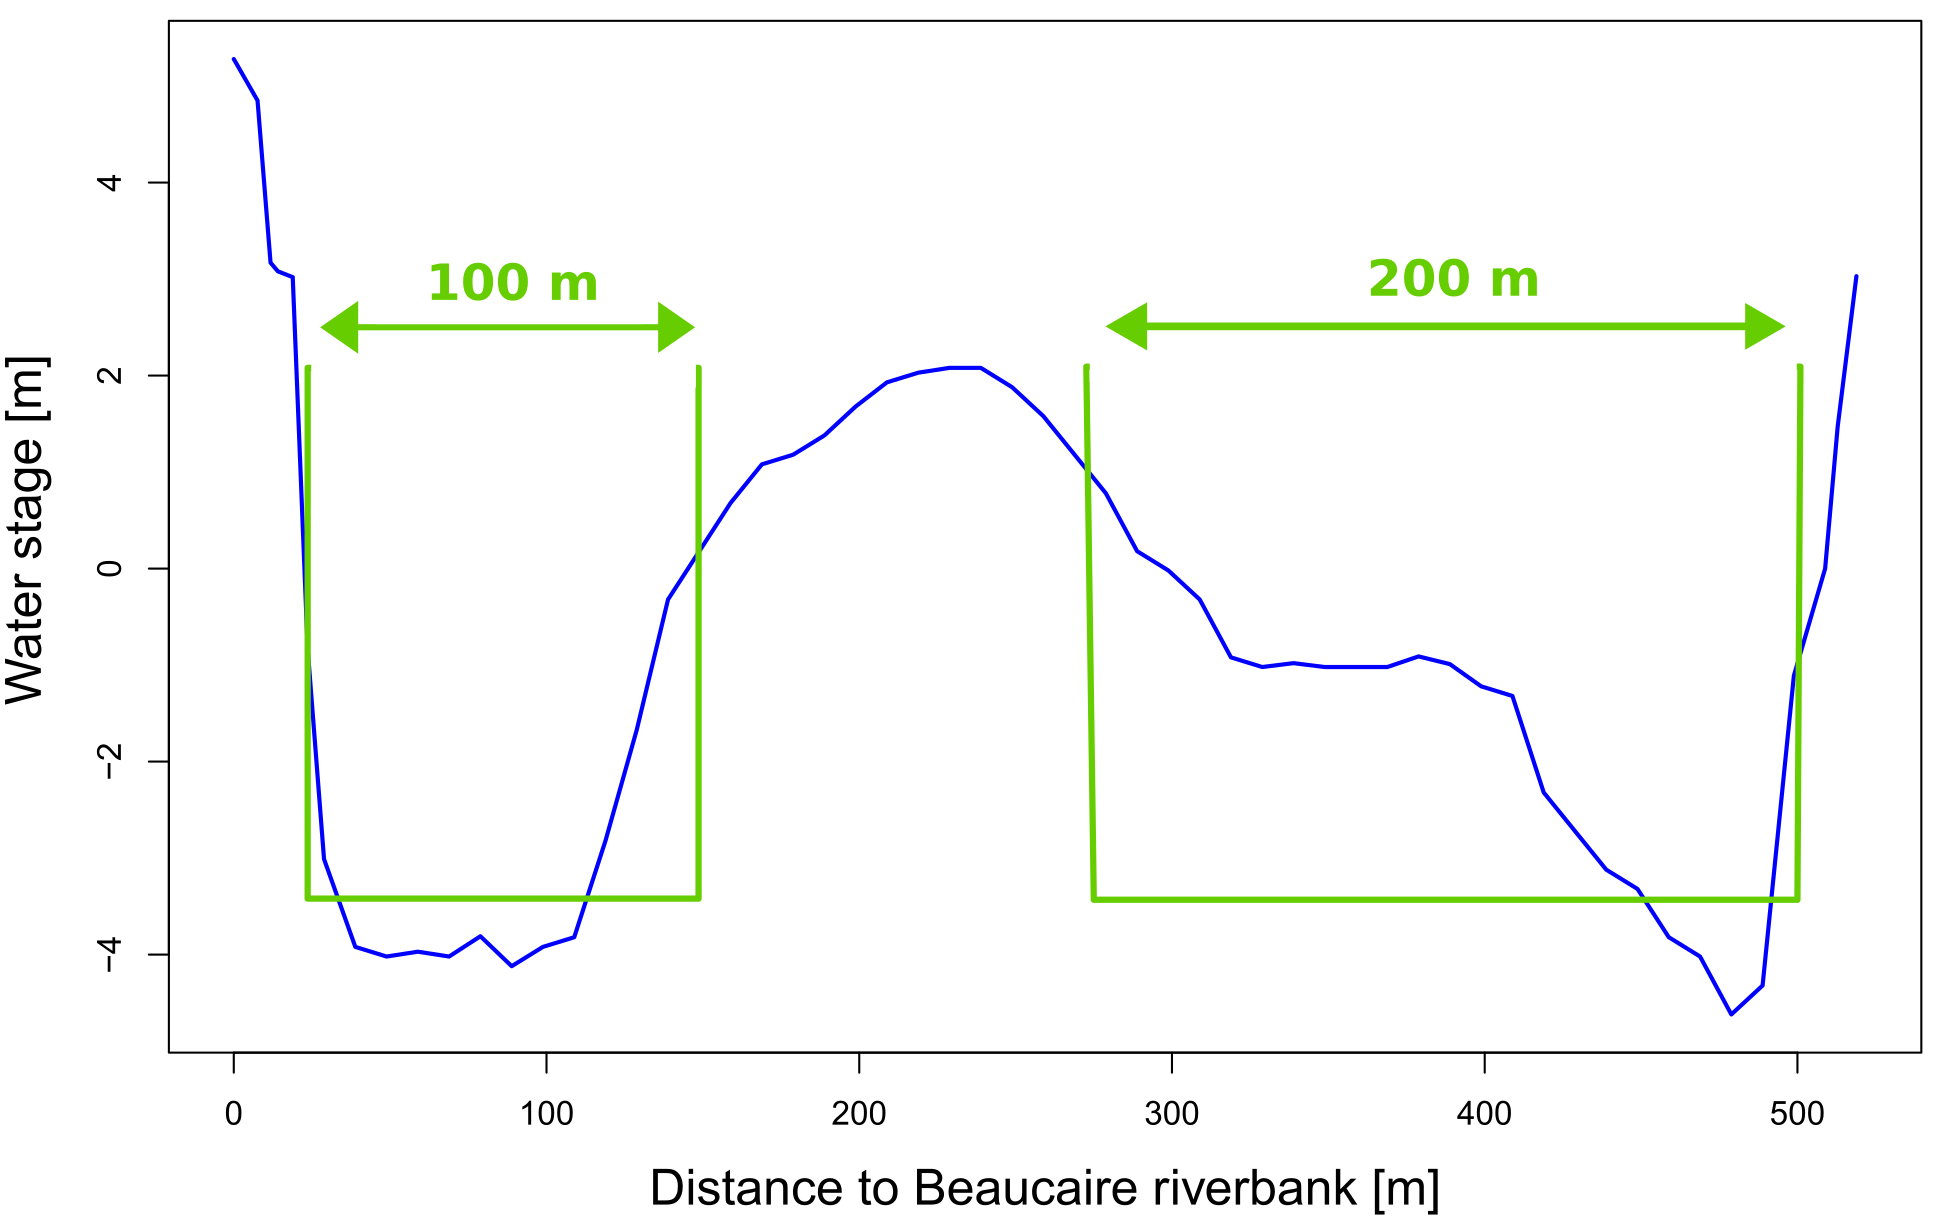
\includegraphics[width=1\linewidth]{Chapitre3/Figures/3b-MatrixChenal_EN.png}
            \caption{}
            \label{subfig:matrixCh}
            \end{subfigure}
            
            \begin{subfigure}{.9\linewidth}
            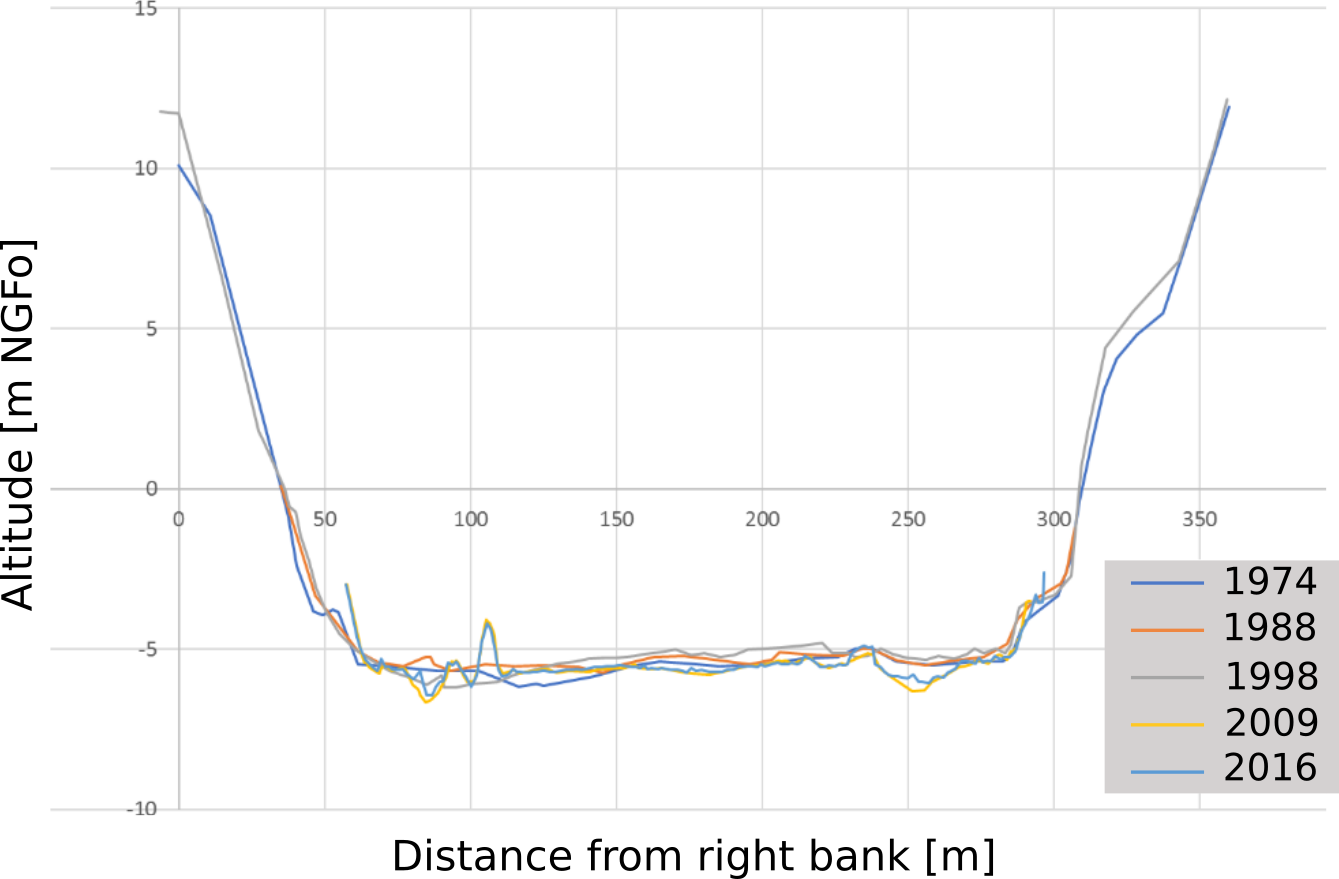
\includegraphics[width=.48\linewidth]{Chapitre3/Figures/3c-ProfilsBardRestit.png}
            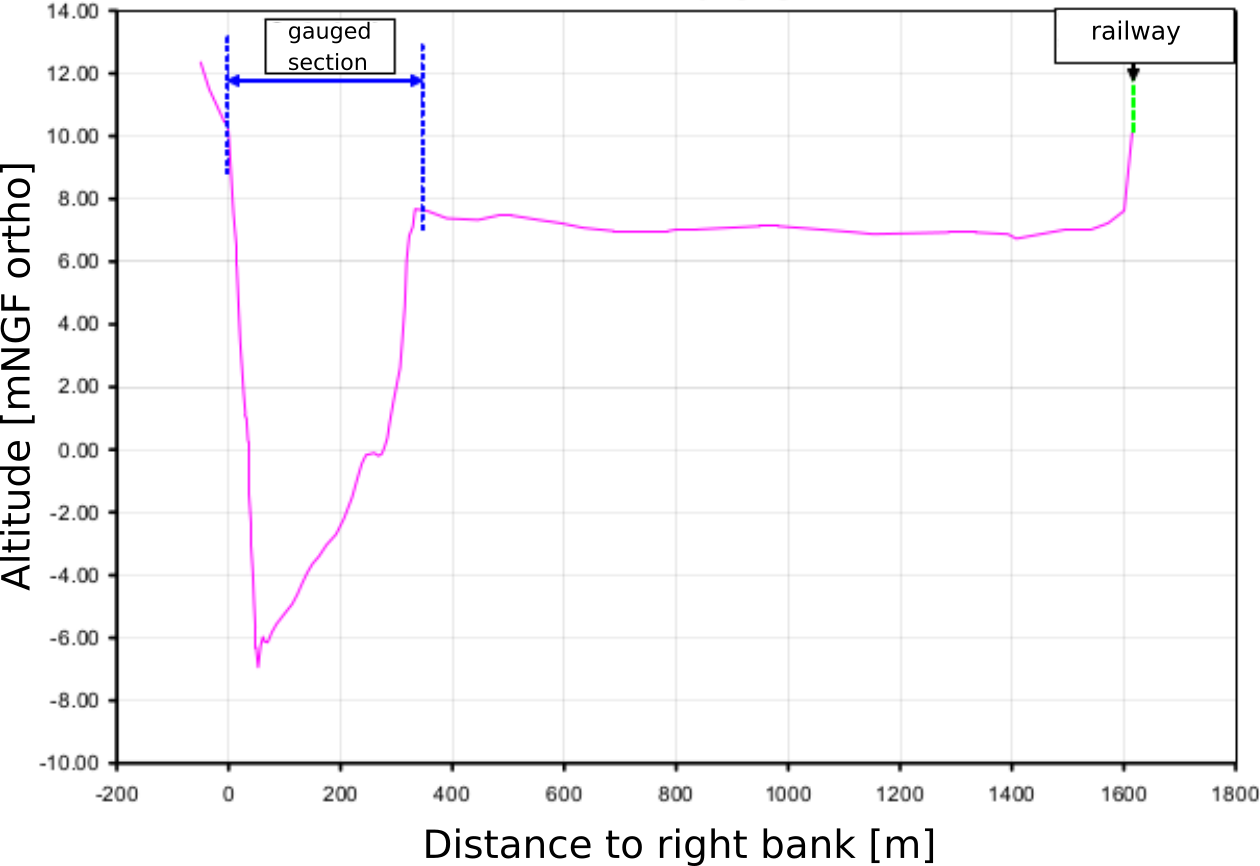
\includegraphics[width=.48\linewidth]{Chapitre3/Figures/3c-ProfilAvalRestitEN.png}
            \caption{}
            \label{subfig:avalprofilesRestit}
            \end{subfigure}
            
            \caption{Historical geometry of the Rhône river near Beaucaire: (a) Map of dike evolution between 18\textsuperscript{th} and 20\textsuperscript{th} centuries, adapted from \citet{armand_ii_1907}; (b) Approximation of the two subchannels composing the main channel control, based on a 1845 cross-section survey; (c) Profiles from 1974 to 2016 (left) at Beaucaire Restitution station and 2.5 km downstream from the station (right) from CNR data, translated from \citet{bard_actualisation_2018} and \citet{medd_debit_2005}}
            \label{fig:groupPriorPt}
        \end{figure}
        % \FloatBarrier


        \subsubsection{Beaucaire Restitution}
        
        Beaucaire Restitution station has a quite stable profile according to 1974-2016 cross-sections (figure \ref{subfig:avalprofilesRestit} left), but the stage-discharge relationship is known to be influenced by the Mediterranean Sea level variations for very low flows (this influence does not apply to the Pont de Beaucaire gauge, located 2 kilometers upstream). This backwater effect can be represented by a channel control with a slope smaller than the slope of the uniform flow, i.e. the mean slope of the channel. The first control (representing low flows influenced by the sea) therefore has the same geometry as the second control (the main channel), but a smaller slope. The main channel control is not influenced by the sea and its slope is close to the longitudinal river slope. 
        \paragraph{}At the gauge location, the 12 meters high banks prevent overbank flows (figure \ref{subfig:avalprofilesRestit} left). However, overbank flows occur further downstream on the left bank, for stages higher than approximately 8 m (figure \ref{subfig:avalprofilesRestit} right). A floodway control (additive to the main channel) is activated above $\approx$ 8 m to model those overbank flows. Therefore, the rating curve equation can be written as follows: 
        
        \begin{equation}
        Q(h) =
          \begin{cases}
           a_1(h-b_1)^{c_1}, & \text{if $\kappa_1 < h \leq \kappa_2 $ (main channel, sea-influenced) }\\
           a_2(h-b_2)^{c_2}, & \text{if $\kappa_2 < h \leq \kappa_3 $ (main channel, non-influenced)}\\
           a_2(h-b_2)^{c_2}+ a_3(h-b_3)^{c_3} & \text{if $h > \kappa_3$ (main channel + floodway)}
          \end{cases}
          \label{eq:RcRes}
        \end{equation}

        Prior distributions of rating curve parameters are specified using recent maps and cross-sections. Priors of the influenced and non-influenced main channels offsets $b_1$ and $b_2$ are assumed Gaussian with mean the riverbed elevation that is approximately equal to -5 m. Those offsets $b_1$ and $b_2$ are assumed changing in parallel (same local changes as the controls are in the same channel) due to a bed erosion trend described in section \ref{sec:stageevolution}, whereas floodway offset $b_3$ and channel widths are supposed constant because of fixed dikes. These "local changes" $\Delta_l^{(k)}$ are computed backwards in time as follows: 

        \begin{equation}
          \begin{cases}
           b_1^{(k)} = b_1^{(k-1)}-\Delta_l^{(k)}, & \text{(incremental changes in the main channel)}\\
           b_2^{(k)} = b_2^{(k-1)}-\Delta_l^{(k)}, & \text{(incremental changes in the floodway)}
          \end{cases}
          \label{eq:SPD_Res}
        \end{equation}
        
        Priors of incremental bed elevation changes are determined in section \ref{sec:stageevolution}.

    \subsubsection{Prior estimation of bed changes}
    \label{sec:stageevolution}
    
    It is possible to follow the evolution of riverbed elevation through the evolution of yearly lowest stages. Here, the 5\% annual stage quantile is considered (figure \ref{fig:quantile5_both}). At Pont de Beaucaire (1816 - 1967), the 5\% quantile is oscillating with a 0.3 m standard deviation. Those variations do not seem to be related to the occurrence of major floods. Without more precise information, we assume that prior distributions of local and overall offset changes defined in section \ref{sec:prior_elicitation} are Gaussian with mean zero and standard deviation 0.3 (table \ref{tab:PriorPt}).
    
    At Beaucaire Restitution (1970-2020), the annual 5\% quantile shows a large decrease during the first 4 years (more than 1 m). This is a consequence of Vallabrègues hydraulic works between 1967 and 1970 as well as substantial dredgings. A geomorphic adjustment after the works in the channel may have affected the riverbed level as well. After the first years, the channel bottom stabilized, however with a slight scouring trend of about 30 cm in 40 years. The standard deviation of the 5\% quantiles reaches 0.5 m. Those bed elevation changes affect both sea-influenced and non-influenced main channel controls offsets. Therefore, the prior distribution of local changes is assumed Gaussian, with mean zero and standard deviation 0.8 m, which is larger than 0.5 m to be more representative of the large changes that occurred during the first years (table \ref{tab:PriorRestit}).
    
    \begin{figure}[h!]
        \centering
        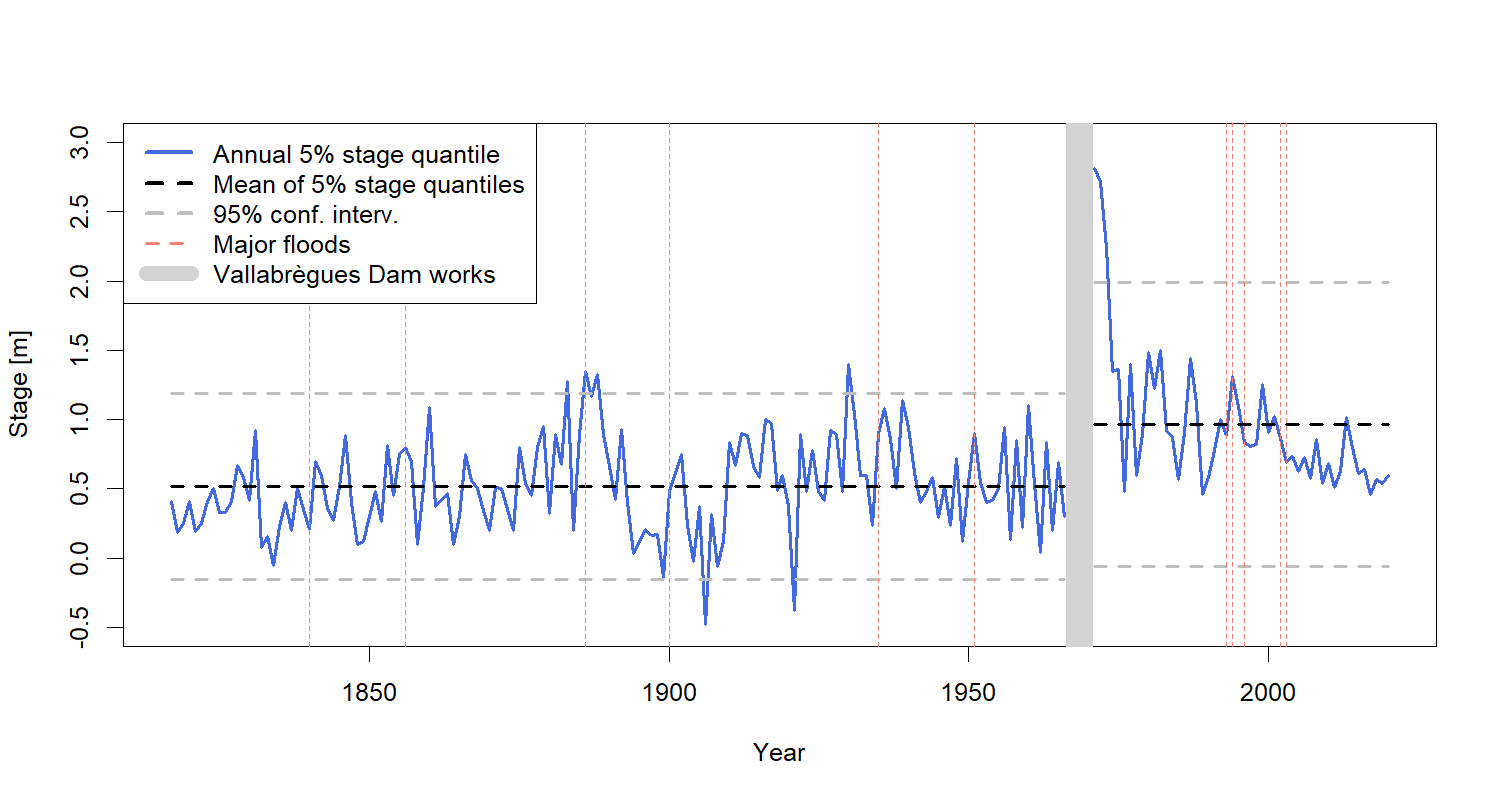
\includegraphics[width = 15cm]{Chapitre3/Figures/5-Quant5perc_both.png}
        \caption{Time series of annual 5\% stage quantile at both Pont de Beaucaire (1816-1967) and Beaucaire Restitution (1970-2020) stations.}
        \label{fig:quantile5_both}
    \end{figure}
    % \FloatBarrier
            
    \begin{table}[h!]
        \begin{tabular}{|l|l|l|l|l|}
            \firsthline
            Physical param. & Meaning & Prior & Inferred param. & Prior\\
            \hline
            \multicolumn{5}{|l|}{\textbf{Control 1: main channel}} \\
            $b_1 [m]$      &   Offset              &  $\mathcal{N}(-4,0.5)$   &     $b_1 [m]$    &  $\mathcal{N}(-4,0.5)$ \\
            \hline
            $B_1 [m]$     &   Channel width   &  $\mathcal{LN}(ln(300),0.16)$&$a_1 [m^{3/2}/s]$  & $\mathcal{LN}(ln(128.6),1.8.10^{-2})$\\
            $K_1 [m^{1/3}/s]$&   Strickler coeff. &  $\mathcal{LN}(ln(35),0.14)$    &                &                     \\
            $S_1 [m/m]$     &   Bed slope        &  $\mathcal{LN}(ln(1.5.10^{-4}),0.55)$         &                &  \\
            \hline
            $c_1 [-]$     &   Exponent            &  $\mathcal{N}(5/3,0.025)$&     $c_1 [-]$     &$\mathcal{N}(5/3,0.025)$\\
            \hline
            \multicolumn{5}{|l|}{\textbf{Control 2: floodway}} \\
            %\hline
            $b_2 [m]$     &   Offset              &  $\mathcal{N}(1.5,0.5)$   &     $b_2 [m]$   &  $\mathcal{N}(2,0.5)$ \\
            \hline
            $B_2 [m]$     &   Channel width   &  $\mathcal{LN}(ln(500),0.1)$  &   $a_2 [m^{3/2}/s]$&  $\mathcal{LN}(ln(241.9),1.10^{-2})$\\
            $K_2 [m^{1/3}/s]$&   Strickler coeff. &  $\mathcal{LN}(ln(30),0.16)$    &                 &                     \\
            $S_2 [m/m]$     &   Bed slope        &   $\mathcal{LN}(ln(2.6.10^{-4}),0.34)$        &                &\\
            \hline
            $c_2 [-]$     &   Exponent           &  $\mathcal{N}(5/3,0.025)$&     $c_2 [-]$    &$\mathcal{N}(5/3,0.025)$\\
            \hline
            \multicolumn{5}{|l|}{\textbf{Structural uncertainty parameters}} \\
            %\hline
            $\gamma_{1} [m^{3}/s]$ & Intercept & $\mathcal{U}(0,1000)$ & $\gamma_{1} [m^{3}/s]$ & $\mathcal{U}(0,1000)$\\
            $\gamma_{2} [-]$ & Slope & $\mathcal{U}(0,100)$ & $\gamma_{2} [-]$ &$\mathcal{U}(0,100)$  \\
            \hline
            \multicolumn{5}{|l|}{\textbf{Multiperiod RC parameters}} \\
            $\Delta l [m]$     &   Local change    &  $\mathcal{N}(0,0.3)$&      $\Delta l [m]$     &$\mathcal{N}(0,0.3)$\\
            $\Delta g [m]$     &   overall change       &  $\mathcal{N}(0,0.3)$&      $\Delta g [m]$     &$\mathcal{N}(0,0.3)$\\
            \lasthline
        \end{tabular} 
        \caption{Priors elicitation for Pont de Beaucaire rating curves. $\mathcal{U}(a,b)$ stands for continuous uniform distribution with bounds $a$ and $b$, $\mathcal{N}(\mu,\sigma)$ for Normal distribution with mean $\mu$  and standard deviation $\sigma$, and $\mathcal{LN}(\mu,\sigma)$ for Log Normal distribution with log-mean $\mu$ and log-standard-deviation $\sigma$.}
        \label{tab:PriorPt}
    \end{table}

    \begin{table}[h!]
        \begin{tabular}{|l|l|l|l|l|}
        \firsthline
            Physical param. & Meaning & Prior & Inferred param. & Prior\\
            \hline
            \multicolumn{5}{|l|}{\textbf{Control 1: Low flows sea-influenced channel}} \\
            $b_1 [m]$      &   Offset              &  $\mathcal{N}(-5,0.5)$   &     $b_1 [m]$    &  $\mathcal{N}(-5,0.5)$ \\
            \hline
            $B_1 [m]$     &   Channel width   &  $\mathcal{LN}(ln(300),0.32)$&$a_1 [m^{3/2}/s]$  & $\mathcal{LN}(ln(49.50),3.2.10^{-2})$\\
            $K_1 [m^{1/3}/s]$&   Strickler coeff. &  $\mathcal{LN}(ln(35),0.14)$    &              &                     \\
            $S_1 [m/m]$     &   Bed slope        &  $\mathcal{LN}(ln(5.10^{-5}),0.20)$         &                  & \\
            \hline
            $c_1 [-]$     &   Exponent            &  $\mathcal{N}(5/3,0.025)$&     $c_1 [-]$     &$\mathcal{N}(5/3,0.025)$\\
            \hline
            \multicolumn{5}{|l|}{\textbf{Control 2: Main channel}} \\
            $b_1 [m]$      &   Offset              &  $\mathcal{N}(-5,0.5)$   &     $b_1 [m]$    &  $\mathcal{N}(0,0.5)$ \\
            \hline
            $B_1 [m]$     &   Channel width   &  $\mathcal{LN}(ln(300),0.32)$& $a_2 [m^{3/2}/s]$  & $\mathcal{LN}(ln(148.49),2.4.10^{-2})$\\
            $K_1 [m^{1/3}/s]$&   Strickler coeff. &  $\mathcal{LN}(ln(35),0.14)$    &              &                     \\
            $S_1 [m/m]$     &   Bed slope        &  $\mathcal{LN}(ln(2.10^{-4}),0.25)$         &              & \\
            \hline
            $c_1 [-]$     &   Exponent            &  $\mathcal{N}(5/3,0.025)$&     $c_2 [-]$     &$\mathcal{N}(5/3,0.025)$\\
            \hline
            \multicolumn{5}{|l|}{\textbf{Control 3: Floodway}} \\
            %\hline
            $b_3 [m]$     &   Offset              &  $\mathcal{N}(8,0.5)$   &     $b_3 [m]$   &  $\mathcal{N}(8,0.5)$ \\
            \hline
            $B_3 [m]$     &   Channel width   &  $\mathcal{LN}(ln(200),0.47)$  &   $a_3 [m^{3/2}/s]$ &  $\mathcal{LN}(ln(241.9),1.10^{-2})$\\
            $K_3 [m^{1/3}/s]$&   Strickler coeff. &  $\mathcal{LN}(ln(25),0.20)$    &              &                     \\
            $S_3 [m/m]$     &   Bed slope        &   $\mathcal{LN}(ln(2.4.10^{-4}),0.21)$        &                      &\\
            \hline
            $c_3 [-]$     &   Exponent           &  $\mathcal{N}(5/3,0.025)$&     $c_3 [-]$    &$\mathcal{N}(5/3,0.025)$\\
            \hline
            \multicolumn{5}{|l|}{\textbf{Structural uncertainty parameters}} \\
            %\hline
            $\gamma_{1} [m^{3}/s]$ & Intercept & $\mathcal{U}(0,1000)$ & $\gamma_{1} [m^{3}/s]$ & $\mathcal{U}(0,1000)$\\
            $\gamma_{2} [-]$ & Slope & $\mathcal{U}(0,100)$ & $\gamma_{2} [-]$ &$\mathcal{U}(0,100)$  \\
            \hline
            \multicolumn{5}{|l|}{\textbf{Multiperiod RC parameters}} \\
            $\Delta l [m]$     &   Local change    &  $\mathcal{N}(0,0.8)$&      $\Delta l [m]$     &$\mathcal{N}(0,0.8)$\\
            \lasthline
            \end{tabular} 
            \caption{Priors elicitation for Beaucaire Restitution rating curves. $\mathcal{U}(a,b)$ stands for continuous uniform distribution with bounds $a$ and $b$, $\mathcal{N}(\mu,\sigma)$ for Normal distribution with mean $\mu$  and standard deviation $\sigma$, and $\mathcal{LN}(\mu,\sigma)$ for Log Normal distribution with log-mean $\mu$ and log-standard-deviation $\sigma$.}
        \label{tab:PriorRestit}
    \end{table}
    \FloatBarrier
    
    \subsection{Stage series}

    \subsubsection{Pont de Beaucaire (1816 - 1967)}
    
    Thanks to the archival work of \citet{pichard_hydro-climatology_2017}, a systematic stage series at Pont de Beaucaire from 1816 to 1967 is available with daily stage readings from 1816 to 1840, and three stage readings per day from 1841 to 1967. The records were made visually by an operator, at noon during the first years, then at 7am, 12am and 5pm (Figure \ref{fig:TabObsPt}). When three stage readings per day are available, the maximum of the three stages is considered as the daily maximum stage, and before 1840 the unique value at noon is kept as the daily maximum stage. Additionally, after 1840, when the stage was rising above 5 m, the operators made more frequent visual records (supposedly hourly measurements). When these records are available, they are of course used to establish the daily maximum stages.
    
        \begin{figure}[h!]
            \centering
            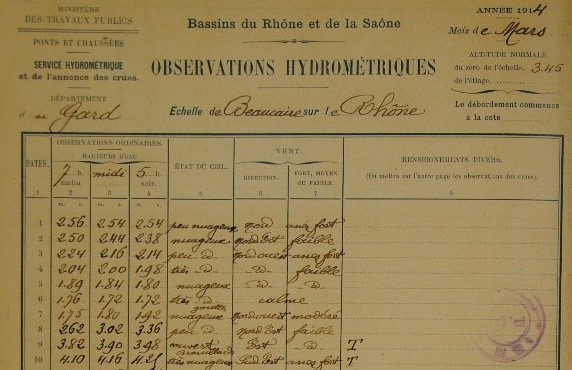
\includegraphics[width = 10cm]{Chapitre3/Figures/4-TabObsBcrSmall.jpg}
            \caption{Table of limnimetric surveys at Pont de Beaucaire, March 1914. Operators were supposed to provide the water level at 7am, 12am and 5pm, as well as a few meteorologic details. \citep{pontschaussees_observations_1914}}
            \label{fig:TabObsPt}
        \end{figure}
        
    Stage uncertainties depend on the measurement method, as described in section \ref{subsec:StageErr}. Table \ref{tab:StageErr} summarizes the different sources of stage uncertainties at Beaucaire, here given as standard deviations $\sigma$. Staff gauge reading uncertainty $\sigma_1$ is taken as 5 cm. Staff gauge precision is centimetric, but as this work is focused on floods, the error is expanded because of the waves that may complicate the reading. 
    Sensor precision $\sigma_2$ and sensor calibration uncertainties $\sigma_3$ are not considered at Pont de Beaucaire as the stage was read by operators directly on the staff gauge. 
    \citet{bard_actualisation_2018} have compiled several elevation measurements of the staff gauge datum between 1912 and 2010. Most of those measurements occurred after the decommissioning of Pont de Beaucaire station. Datum uncertainty $\sigma_4$ is assumed to be equal to the standard deviation of those measurements: 6 cm. The datum measurement frequency during the operation of Pont de Beaucaire station is assumed to be 25 years (i.e. the average duration between the retrieved elevation measurements). Hence, datum errors are drawn every 25 years. 
    As described in section \ref{subsec:StageErr}, the distribution of measurement frequency errors $\delta_5$ can be estimated using the frequent stage measurements at Beaucaire Restitution between 1970 and 2020 (50 AMAX values). For the "one stage reading per day" case (mimicking the 1816-1840 period), this error corresponds to the difference between the maximum hourly stage value and the stage at noon of the same day. The "three stage readings per day" error (1840-1967) is the difference between the maximum hourly stage of a day, and the maximum of 7am, noon and 5pm stages of the same day. An exponential distribution is estimated for both errors samples and is used to represent the measurement frequency uncertainty affecting the annual maximum stages at Pont de Beaucaire. According to gauge management instructions, hourly measurements were made by observers after 1840, and for the stages above 5 meters. Hence, measurement frequency error $\delta_5$ can be considered as negligible when stage is above 5 meters after 1840.
    \paragraph{}
    \citet{symadrem_programme_2012}, \citet{pichard_hauteurs_2013} and \citet{bard_actualisation_2018} suggested that for the floods during which dike breaks happened downstream from Beaucaire, stage measurements should be corrected because the stage measured at the station may lead to underestimating the actual discharge of the flood. The stage corrections for the more thoroughly studied floods of 1840, 1841 and 1856 estimated by \citet{symadrem_programme_2012} are adopted. For these floods stage uncertainty is represented by a Gaussian distribution, with mean the estimated stage and standard deviation half of the applied correction, chronologically: 0.94, 0.4 and 0.4 m. 
    \FloatBarrier
 
    \subsubsection{Beaucaire Restitution (1970 - 2020)}
    
    For Beaucaire Restitution station, most of the stage uncertainty values come from \citet{cetiat_conference_2005} expertise on behalf of Compagnie Nationale du Rhône. They are summarized in table \ref{tab:StageErr}. Staff gauge reading uncertainty is considered zero as the measurements are done by automatic sensors. Instrument precision uncertainty: $\sigma_2 = 0.01/\sqrt{3}$ m comes from the sensor manufacturer specifications. The standard deviation of all the re-calibrations made by the operators is equal to 5 cm according to \citet{cetiat_conference_2005}. Calibration is also affected by staff gauge reading uncertainties, because the stage read on the staff gauge is the reference used by operators to calibrate the sensor. \citet{cetiat_conference_2005} estimated a 3.35 cm uncertainty for the gauge reading uncertainty. Therefore, gauge reading and calibration uncertainties are combined as follows: $\sigma_3 = \sqrt{0.0335^2 + 0.05^2} = 0.06$ m. As the average time lag between calibrations is 6 months, a new value of the error $\delta_3$ is drawn for each annual maximum stage. Datum reference uncertainty $\sigma_4$ is considered negligible because of the precision of modern topographic measurements ($<1$ cm). Measurement frequency uncertainty $\sigma_5$ is considered negligible, because the sub-hourly measurement frequency is assumed adequate to capture the Rhône River stage variability. 
        
    \begin{table}[h!]
    \centering
    \resizebox{\columnwidth}{!}{%
    \begin{tabular}[c]{|c|c|c|c|c|cc|}
    \hline
    \multirow{2}{*}{\textbf{Date}} &
      \multirow{2}{*}{\textbf{\begin{tabular}[c]{@{}c@{}}$\boldsymbol{\delta_1}$: gauge\\ reading\end{tabular}}} &
      \multirow{2}{*}{\textbf{\begin{tabular}[c]{@{}c@{}}$\boldsymbol{\delta_2}$: sensor \\ precision\end{tabular}}} &
      \multirow{2}{*}{\textbf{\begin{tabular}[c]{@{}c@{}}$\boldsymbol{\delta_3}$: sensor\\ calibration\end{tabular}}} &
      \multirow{2}{*}{\textbf{\begin{tabular}[c]{@{}c@{}}$\boldsymbol{\delta_4}$: datum\\ reference\end{tabular}}} &
      \multicolumn{2}{c|}{\textbf{\begin{tabular}[c]{@{}c@{}}$\boldsymbol{\delta_5}$:\\ measurement frequency\end{tabular}}} \\ \cline{6-7} 
     &
       &
       &
       &
       &
      \multicolumn{1}{c|}{\textbf{Stage\textless5m}} &
      \textbf{Stage$\geq$5m} \\ \hline
    \textbf{Before 1840} &
       $\mathcal{N}(0,0.05)$ &
      - &
      - &
       $\mathcal{N}(0,0.06)$ &
      \multicolumn{2}{c|}{$Exp(2.18)$} \\ \hline
    \textbf{1840 - 1967} &
      $\mathcal{N}(0,0.05)$ &
      - &
      - &
       $\mathcal{N}(0,0.06)$ &
      \multicolumn{1}{c|}{\begin{tabular}[c]{@{}c@{}}$Exp(8.86)$\end{tabular}} &
      - \\ \hline
    \textbf{1970 - 2020} &
       - &
       $\mathcal{N}(0, 0.01/\sqrt{3})$ &
       $\mathcal{N}(0,0.06)$ &
      - &
      \multicolumn{2}{c|}{-} \\ \hline
    \end{tabular}%
    }
    \caption{Distributions used for the different sources of stage errors (in meters). $\mathcal{N}$(mean, st. deviation) and $Exp$(rate) represent Gaussian and Exponential distributions. As a reminder, the periods before 1967 are associated with the Pont de Beaucaire station and the period 1970-2020 with the Beaucaire Restitution station}
    \label{tab:StageErr}
    \end{table}
    \FloatBarrier
    
    \subsection{Gaugings (discharge measurements)}

    \paragraph{}
    A set of 244 gaugings from 1840 to 1967 has been compiled at Pont de Beaucaire. After excluding a few gaugings which were considered dubious, 233 measurements remain. The frequency of gaugings is variable in time. No gaugings were retrieved before 1840 and there are several 10- to 20-year gaps without gaugings, which makes the estimation of the stage-discharge relationship over time challenging. The assumed uncertainty of the gaugings at Beaucaire depends on the gauging method according to \citet{bard_actualisation_2018} values specified in table \ref{TabIcJau}.
    
    \paragraph{}    
    A set of 304 gaugings is available at Beaucaire Restitution. A few of these were out of the period of stage measurements availability and were discarded. Finally, 296 gaugings were selected. As modern hydrometric developments allowed estimating the uncertainty for each individual gauging (particularly for ADCP and current meters), those values are used when available in the CNR archives. If not, values from table \ref{TabIcJau} are considered. 
        
         \begin{table}[ht]
            \centering
                \begin{tabular}{| l | l |} 
                        \hline
                        \textbf{Gauging method} & \textbf{Standard uncertainty} \\
                        \hline
                        Current meter at 0.6 h and surface & 5\% \\
                        \hline
                        Current meter point by point & 3.5\% \\
                        \hline
                        Surface current meter & 7.5\% \\
                        \hline
                        Unknown type & 7.5\% \\
                        \hline
                        ADCP & 3.5\% \\
                        \hline
                        Floats before 1936 & 10\% \\
                        \hline
                        Hydrotachymeter before 1936 & 10\%\\
                        \hline
                \end{tabular}
            \caption{Gaugings uncertainty depending on the method used (hypotheses from \citet{bard_actualisation_2018}). Expressed as standard deviations of the measured discharge in \%.}
            \label{TabIcJau}
        \end{table}
         \FloatBarrier
 \section{Results}
 \label{sec:Results}
 
    \subsection{Assessment of rating shifts}

    \citet{darienzo_detection_2021} segmentation procedure is applied at Beaucaire as described in section \ref{subsec:RatingShifts}. The prior for the residual mean during each sub-period is taken as a Gaussian distribution with zero mean and a 500 m\textsuperscript{3}/s standard deviation for both stations. The maximum number of segments at each iteration is fixed at six (see \citet{darienzo_detection_2021} for details on priors and parameters specification).

    \begin{figure}[h!]
        \centering
        \begin{subfigure}{0.75\textwidth}
        	\centering
        	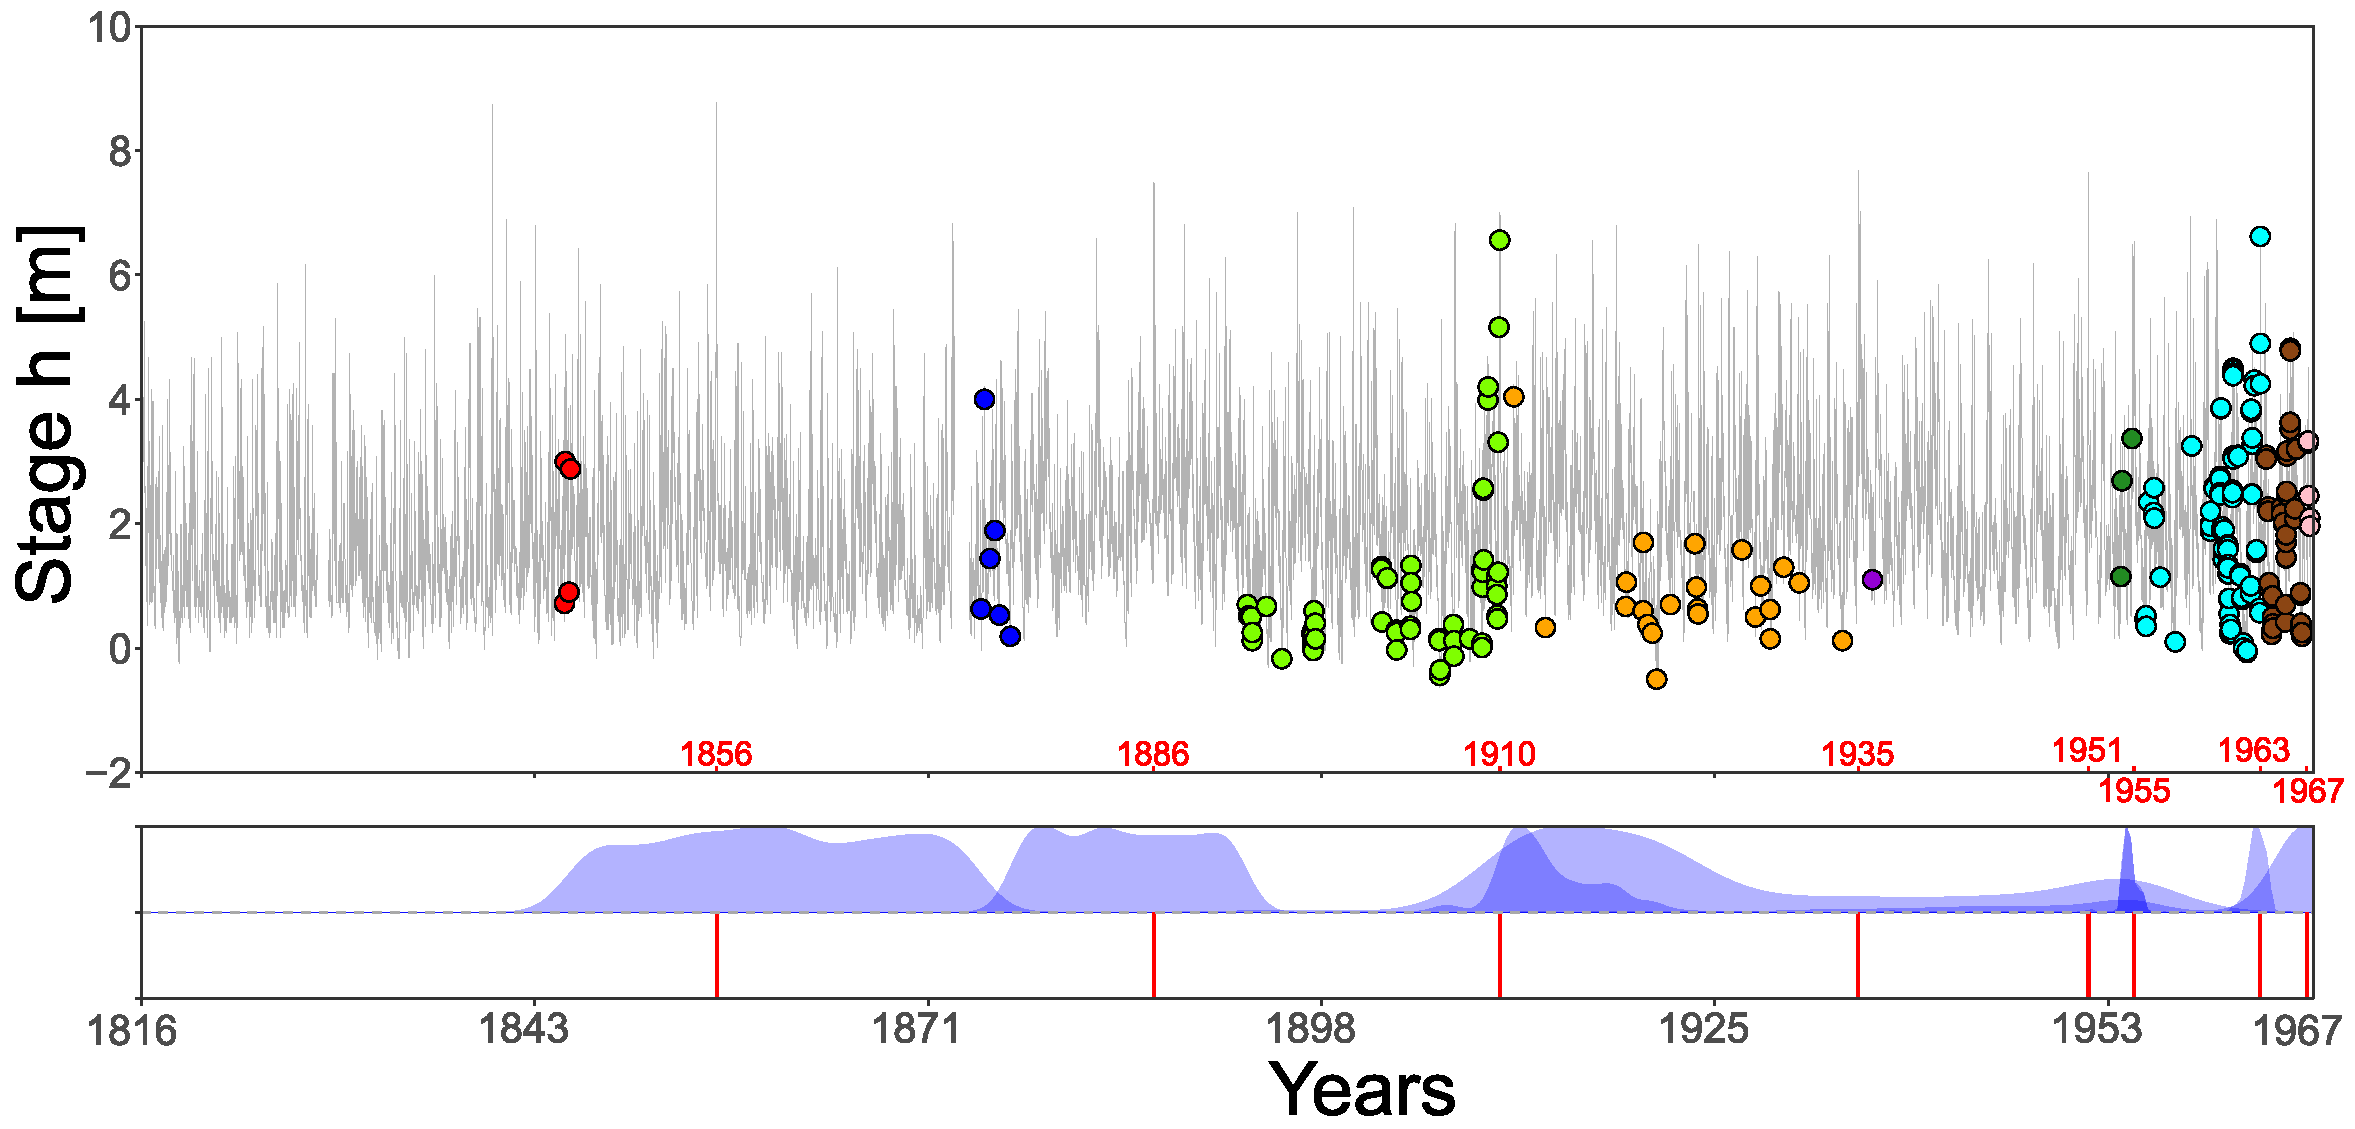
\includegraphics[width = 1\linewidth]{Chapitre3/Figures/6a-SegmPt.pdf}
        	\caption{}
		\end{subfigure}
		\begin{subfigure}{0.75\textwidth}
        	\centering
        	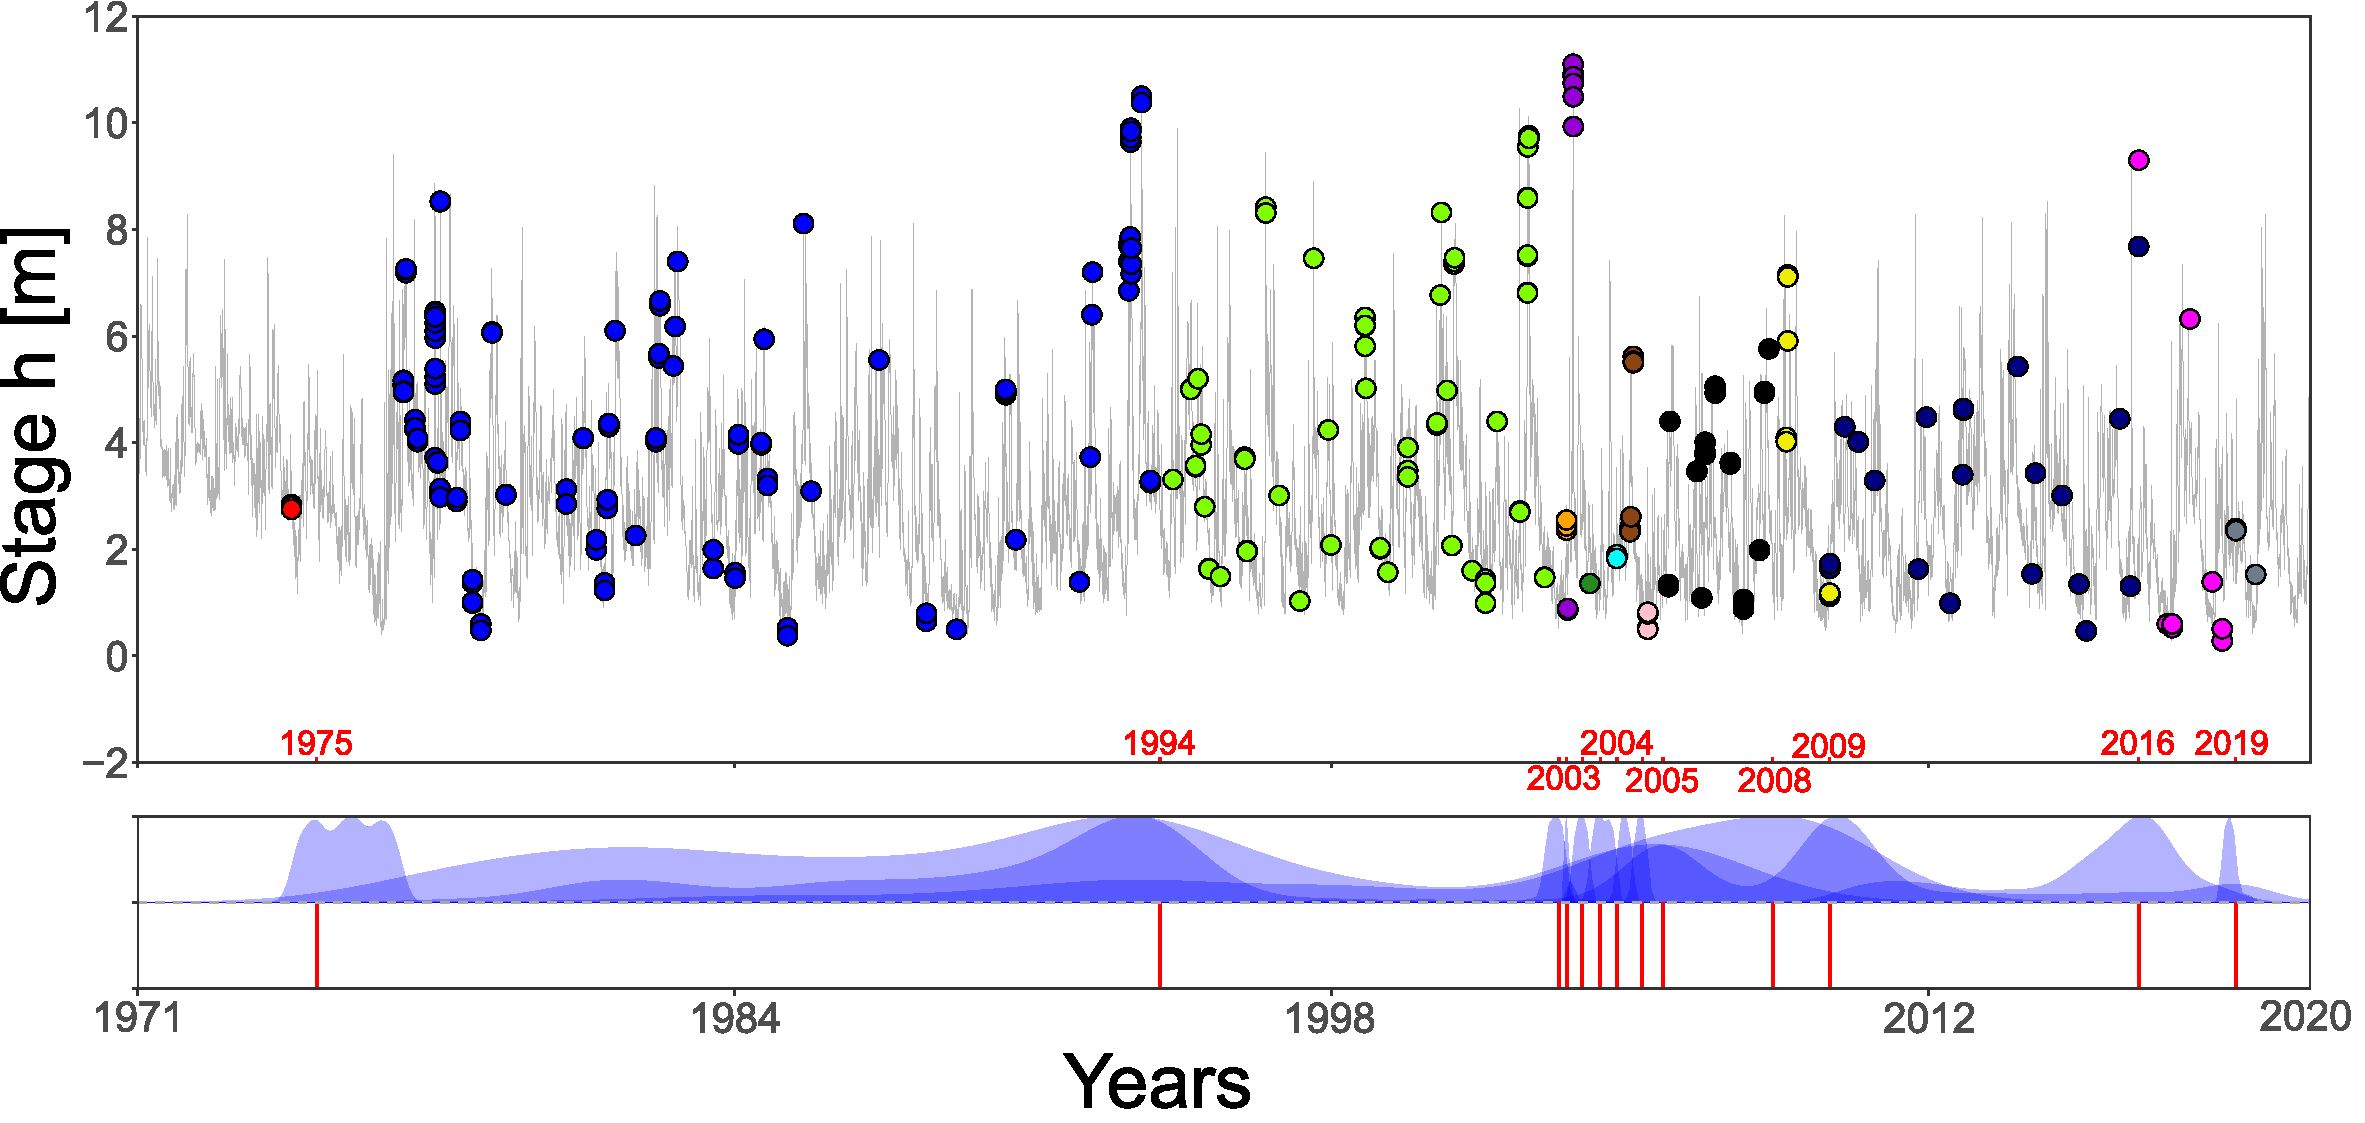
\includegraphics[width = 1\linewidth]{Chapitre3/Figures/6b-SegmRes.pdf}
        	\caption{}
		\end{subfigure} 
		\caption{Gaugings segmentation of the Rhône River at Pont de Beaucaire (a) and Beaucaire Restitution (b). Dots represent gaugings with different colors for each stable period. The grey curve is the stage series. Blue ribbons represent posterior pdf of shift times and red segments are the retained shift times taken as the maximum stage included in each posterior pdf interval.}
        \label{fig:SegmBoth}
    \end{figure}
    
    \paragraph{}
    Eight shift times are detected at Pont de Beaucaire (Figure \ref{fig:SegmBoth} (a)). The gauging frequency is not constant through the history of the station and some periods include a small number of gaugings. As a consequence, the posterior pdfs of shift times span over many years for the first shifts, and are similar to uniform distributions between sets of gaugings. Without discharge measurement (gaugings) the method is not able to detect any rating shifts. Additional information may be of interest for those first periods. It is no surprise that most of the shifts occur very close to the largest historical floods. 1935 and 1951 shifts respectively correspond to the 3\textsuperscript{rd} and 4\textsuperscript{th} largest floods of the history of the station. There is, by construction of the segmentation model, no shift before 1845, year of the first available gaugings. However, we can consider that the 1840 flood (supposedly the largest flood since 1800) is likely to have caused a shift. Therefore, an additional shift time is added at the exact flood date. This brings the total number of stable periods to 10 (table \ref{tab:ShiftDates}). 
    
    \paragraph{}    
    Thirteen shift times are detected at Beaucaire Restitution. As can be seen in figure \ref{fig:SegmBoth} (b), gauging frequency is far higher than for Pont de Beaucaire station (except during the first 5 years), resulting in a better determination of the rating shift times. 
    Due to the lack of gaugings at the beginning of the series, only one rating shift is detected but many shifts potentially took place in those first four years as morphological adjustment and dredging occurred (see section \ref{sec:stageevolution}). This first shift is assumed to be assigned to the first large flood of the station in 1976, after which the channel stabilized. The next shift occurred during the 1994 flood, one of the largest at the station. The most notable flood at Beaucaire Restitution occurred in 2003 (11 500 m\textsuperscript{3}/s, with a return period of about 100 years according to \citet{medd_debit_2005}). Unsurprisingly, the stage-discharge relationship is considerably disrupted by this event, as reflected by the six rating shifts detected from 2003 to 2005. Two out of these six shifts were discarded because the shift amplitude is considered minor based on further analysis of the corresponding rating curve change. The largest flood within posterior intervals of those shifts almost always corresponds to the 2003 flood. This is also the case for 2005, 2008 and 2009 shifts, for which the posterior pdf spans many years including 2003. Therefore, the shift dates are assumed to be located to the maxpost shift times, as several shifts cannot be located at the same date. The last shift of 2019 is also discarded because the shift amplitude is considered minor based on further analysis. Finally, ten rating shifts are retained. This brings the number of stable periods to eleven for Beaucaire Restitution (table \ref{tab:ShiftDates}). 
    \FloatBarrier

    \begin{center}
        \begin{table}[h!]
        \centering
            \begin{tabular}{|m{2.5cm}|m{3.5cm}|m{3.5cm}|m{1.5cm}|m{2.2cm}|}
                \firsthline
                \textbf{Maxpost shift time}  &  \textbf{Largest flood within \textit{post. pdf}} &  \textbf{Final choice} & \textbf{Period number} & \textbf{Number of gaugings}  \\
                \hline
                \multicolumn{5}{|l|}{\textbf{Pont de Beaucaire (1816-1967)}} \\
                \hline
                No gaugings     &      No gaugings   &   1840-11-02 & 1 & 0 \\
                \hline
                1860-02-20     &       1856-06-01  &   1856-06-01   & 2 & 4 \\
                \hline
                1887-05-11     &       1886-10-29  &   1886-10-29   & 3 & 6\\
                \hline
                1910-11-21     &       1910-12-09  &   1910-12-09  & 4 & 58 \\
                \hline
                1921-06-22     &       1935-11-14  &   1935-11-14   & 6 & 22 \\
                \hline
                1954-08-08    &       1951-11-23  &   1951-11-23   & 6 & 1\\
                \hline
                1954-03-30     &       1955-01-23  &   1955-01-23   & 7 & 3 \\
                \hline
                1963-03-23     &       1963-11-08  &   1963-11-08   & 8 & 91 \\
                \hline
                1967-01-31     &       1967-01-31  &   1967-01-31  & 9 & 43\\
                \hline
                1967-12-31      &       End of stage series & End of stage series & 10 & 5\\
                \hline
                \multicolumn{5}{|l|}{\textbf{Beaucaire restitution (1970-2020)}} \\
                \hline
                1975-02-06     &       1976-11-11  &   1976-11-11 & 1 & 3\\
                \hline
                1994-06-10     &       1994-01-08  &   1994-01-08   & 2 & 122 \\
                \hline
                2003-08-05     &       2002-11-27  &   2002-11-27  & 3 & 65 \\
                \hline
                2003-10-09     &       2003-12-04  &   2003-12-04   & 4 & 17 \\
                \hline
                2004-02-16     &       2003-12-04  &   No shift   & X & X \\
                \hline
                2004-07-15     &       2003-12-04  &   2004-07-15   & 5 & 1 \\
                \hline
                2004-12-02     &       2004-12-02  &   2004-12-02   & 6 & 2 \\
                \hline
                2005-07-03     &       2004-12-02  &   No shift  & X & X \\
                \hline
                2005-12-24     &       2003-12-04  &   2005-12-24  & 7 & 14 \\
                \hline
                2008-06-28     &       2003-12-04  &   2008-06-28    & 8 & 28 \\
                \hline
                2009-10-20     &       2003-12-04  &   2009-10-20   & 9 & 7 \\
                \hline
                2016-11-21     &       2016-11-22  &   2016-11-22  & 10 & 26 \\
                \hline
                2019-02-11     &       2018-11-24  &   No shift   & X & X \\
                \hline
                2020-01-01     &      End of stage series  &   End of stage series  & 11 & 11\\
                \lasthline
            \end{tabular}
            
            \caption{Beaucaire rating shifts dates}
            \label{tab:ShiftDates}
        \end{table}
    \end{center}
     \FloatBarrier
    
    \subsection{Multiperiod rating curves estimation}

    \paragraph{}
    Uncertain rating curves are estimated using \citet{mansanarez_shift_2019} SPD model, for each stable period detected previously. For Pont de Beaucaire, this leads to ten rating curves that show a good adequacy with gaugings (figure \ref{subfig:RcPt}). The evolution of the main channel offset ($b_1$) gives indications on the evolution of bed elevation (figure \ref{subfig:B'sPt}). Substantial changes occurred before and after the third stable period with successive increase and decrease of the offset. Those changes may be related to the channel works that occurred during the end of the XIX\textsuperscript{th} Century. Afterwards, the offset is more stable and only suggests a slight increasing trend which may be a consequence of the filling of the channel noticed in figure \ref{fig:quantile5_both}. The widest uncertainty interval belongs to the first period (1816-1840: dark red) for which no gaugings are available (figure \ref{subfig:RcPt}). The expected range of rating curve uncertainties for flood discharges (above 6 m) varies from around 20\% for the first period, to less than 10\% after 1840. Static parameters are precisely estimated and are presented in figure \ref{subfig:a's and c's Pt}. The $c$ posterior distributions are as wide as priors because $c$ priors are already very precise as they come from simplified Manning-Strickler formula for which the exponent is exactly $5/3$.
    
    \paragraph{}
    Eleven uncertain rating curves were computed at Beaucaire Restitution (figure \ref{subfig:RcRes}). The rating curve uncertainty intervals are smaller than at Pont de Beaucaire for usual stages because of a larger number of gaugings and a smaller gaugings uncertainty: around 5\% of uncertainty is estimated for floods above 6 m. However, low flows uncertainty is greater than at Pont de Beaucaire, because the sustained flows of the Rhône River limits the exploration of the sea-influenced hydraulic control. Low flows gaugings are unavailable. Thus, the first control offsets $b_1$ are not precisely estimated (figure \ref{subfig:B'sRes}), but this has no consequences on the streamflow uncertainty of AMAX floods, for which only controls 2 and 3 are active. The first period rating curve (dark red) is shifted with respect to the other curves due to the channel adjustment and dredging operations after Vallabrègues works (1967-1970). The second control offsets ($b_2$) globally decreases over time, showing a slight scouring trend of the channel (figure \ref{subfig:B'sRes}). Static parameters (figure \ref{subfig:bac'sRes}) appear precisely estimated, except for the 3\textsuperscript{rd} control offset $b_3$ for which the posterior distribution is as wide as the prior. 
    
    \paragraph{}
There are several reasons for the significant differences between the upper parts of the rating curves for Pont de Beaucaire (figure \ref{subfig:RcPt}) and Beaucaire Restitution (figure \ref{subfig:RcRes}). First, the gauge datum (the altitude of the stream gauge zero value) correspond to 3.37 m for Pont de Beaucaire and 0.06 m for Beaucaire Restitution. In addition, as the stations are 2 km apart, their cross-sections are very different. Pont de Beaucaire cross-section corresponds to a main channel splitted in two sub-channels (figure \ref{subfig:matrixCh}), while Beaucaire Restitution cross-section corresponds to a unique channel (figure \ref{subfig:avalprofilesRestit}). A magnified representation of the upper parts of the rating curves is available in supplementary material (figure 2).
	
	
    \begin{figure}[h!]
    \centering
        \begin{subfigure}{0.49\textwidth}
            \centering
            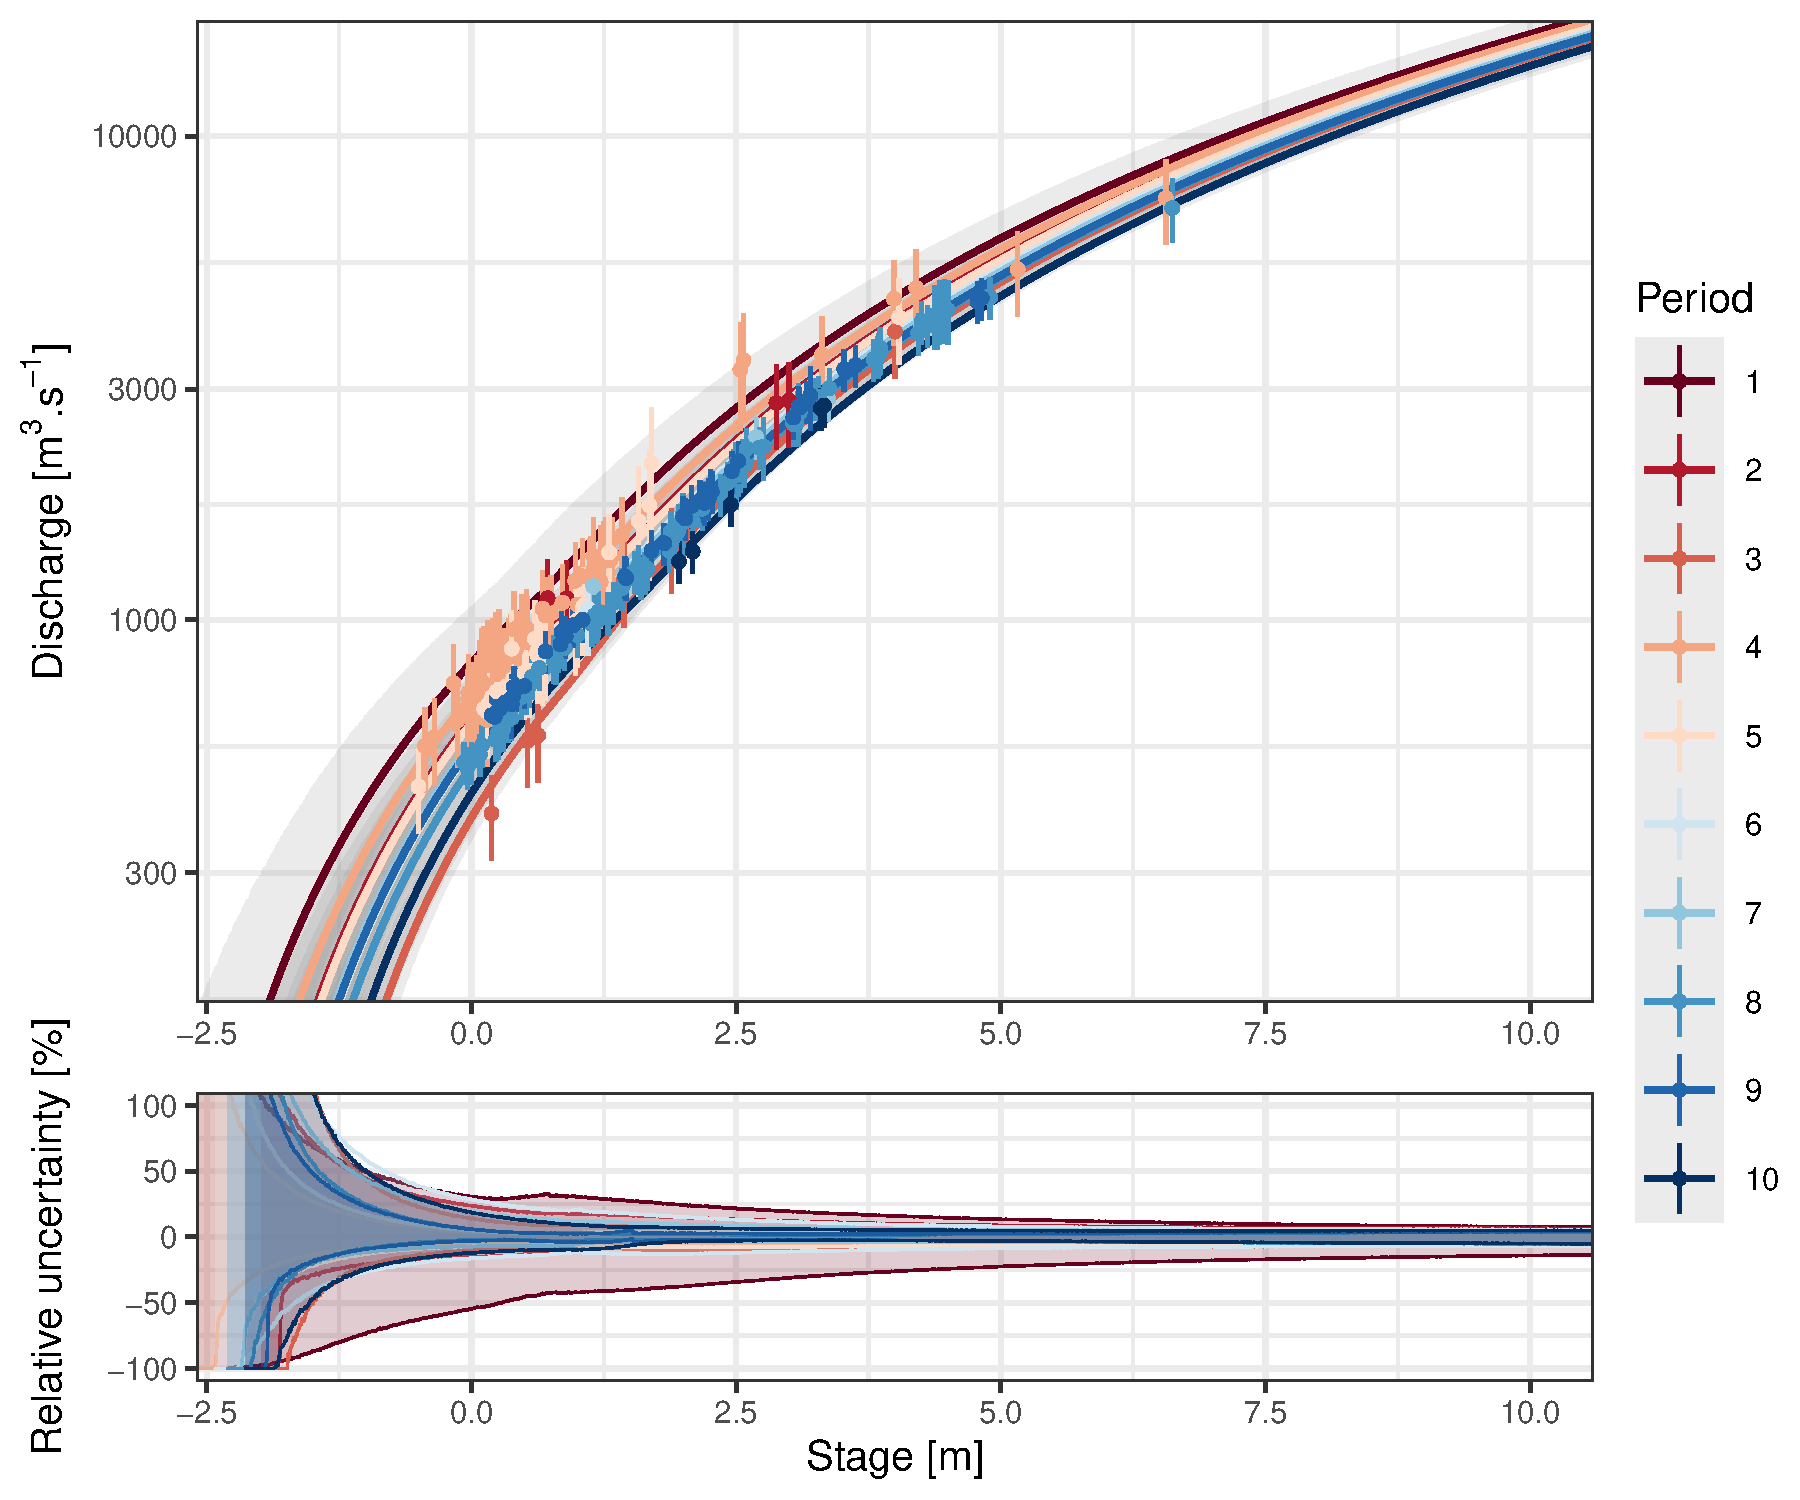
\includegraphics[width=\linewidth]{Chapitre3/Figures/7a-RClog_ICdownPt.pdf}
            \caption{}
            \label{subfig:RcPt}
        \end{subfigure}
        \begin{subfigure}{0.49\textwidth}
            \centering
            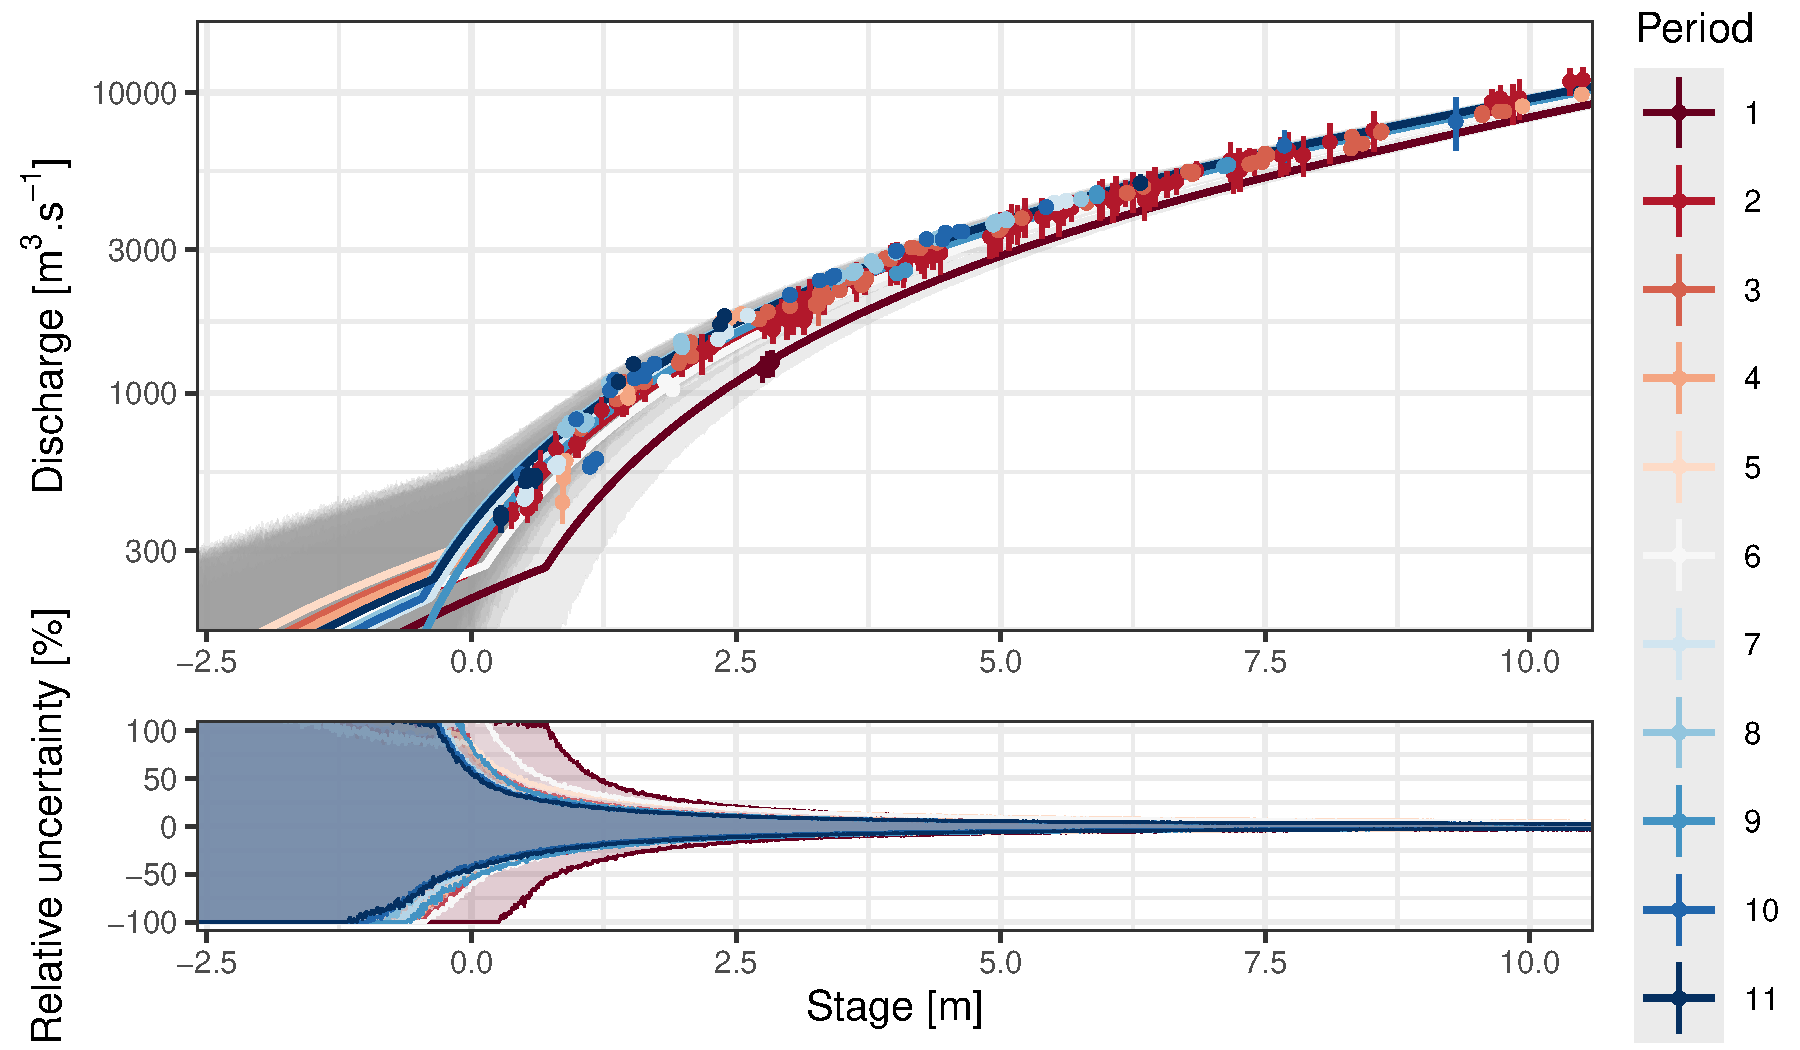
\includegraphics[width=\linewidth]{Chapitre3/Figures/7b-RClog_ICdownRes.pdf}
            \caption{}
            \label{subfig:RcRes}
        \end{subfigure}
        
        \begin{subfigure}{0.48\textwidth}
            \centering
            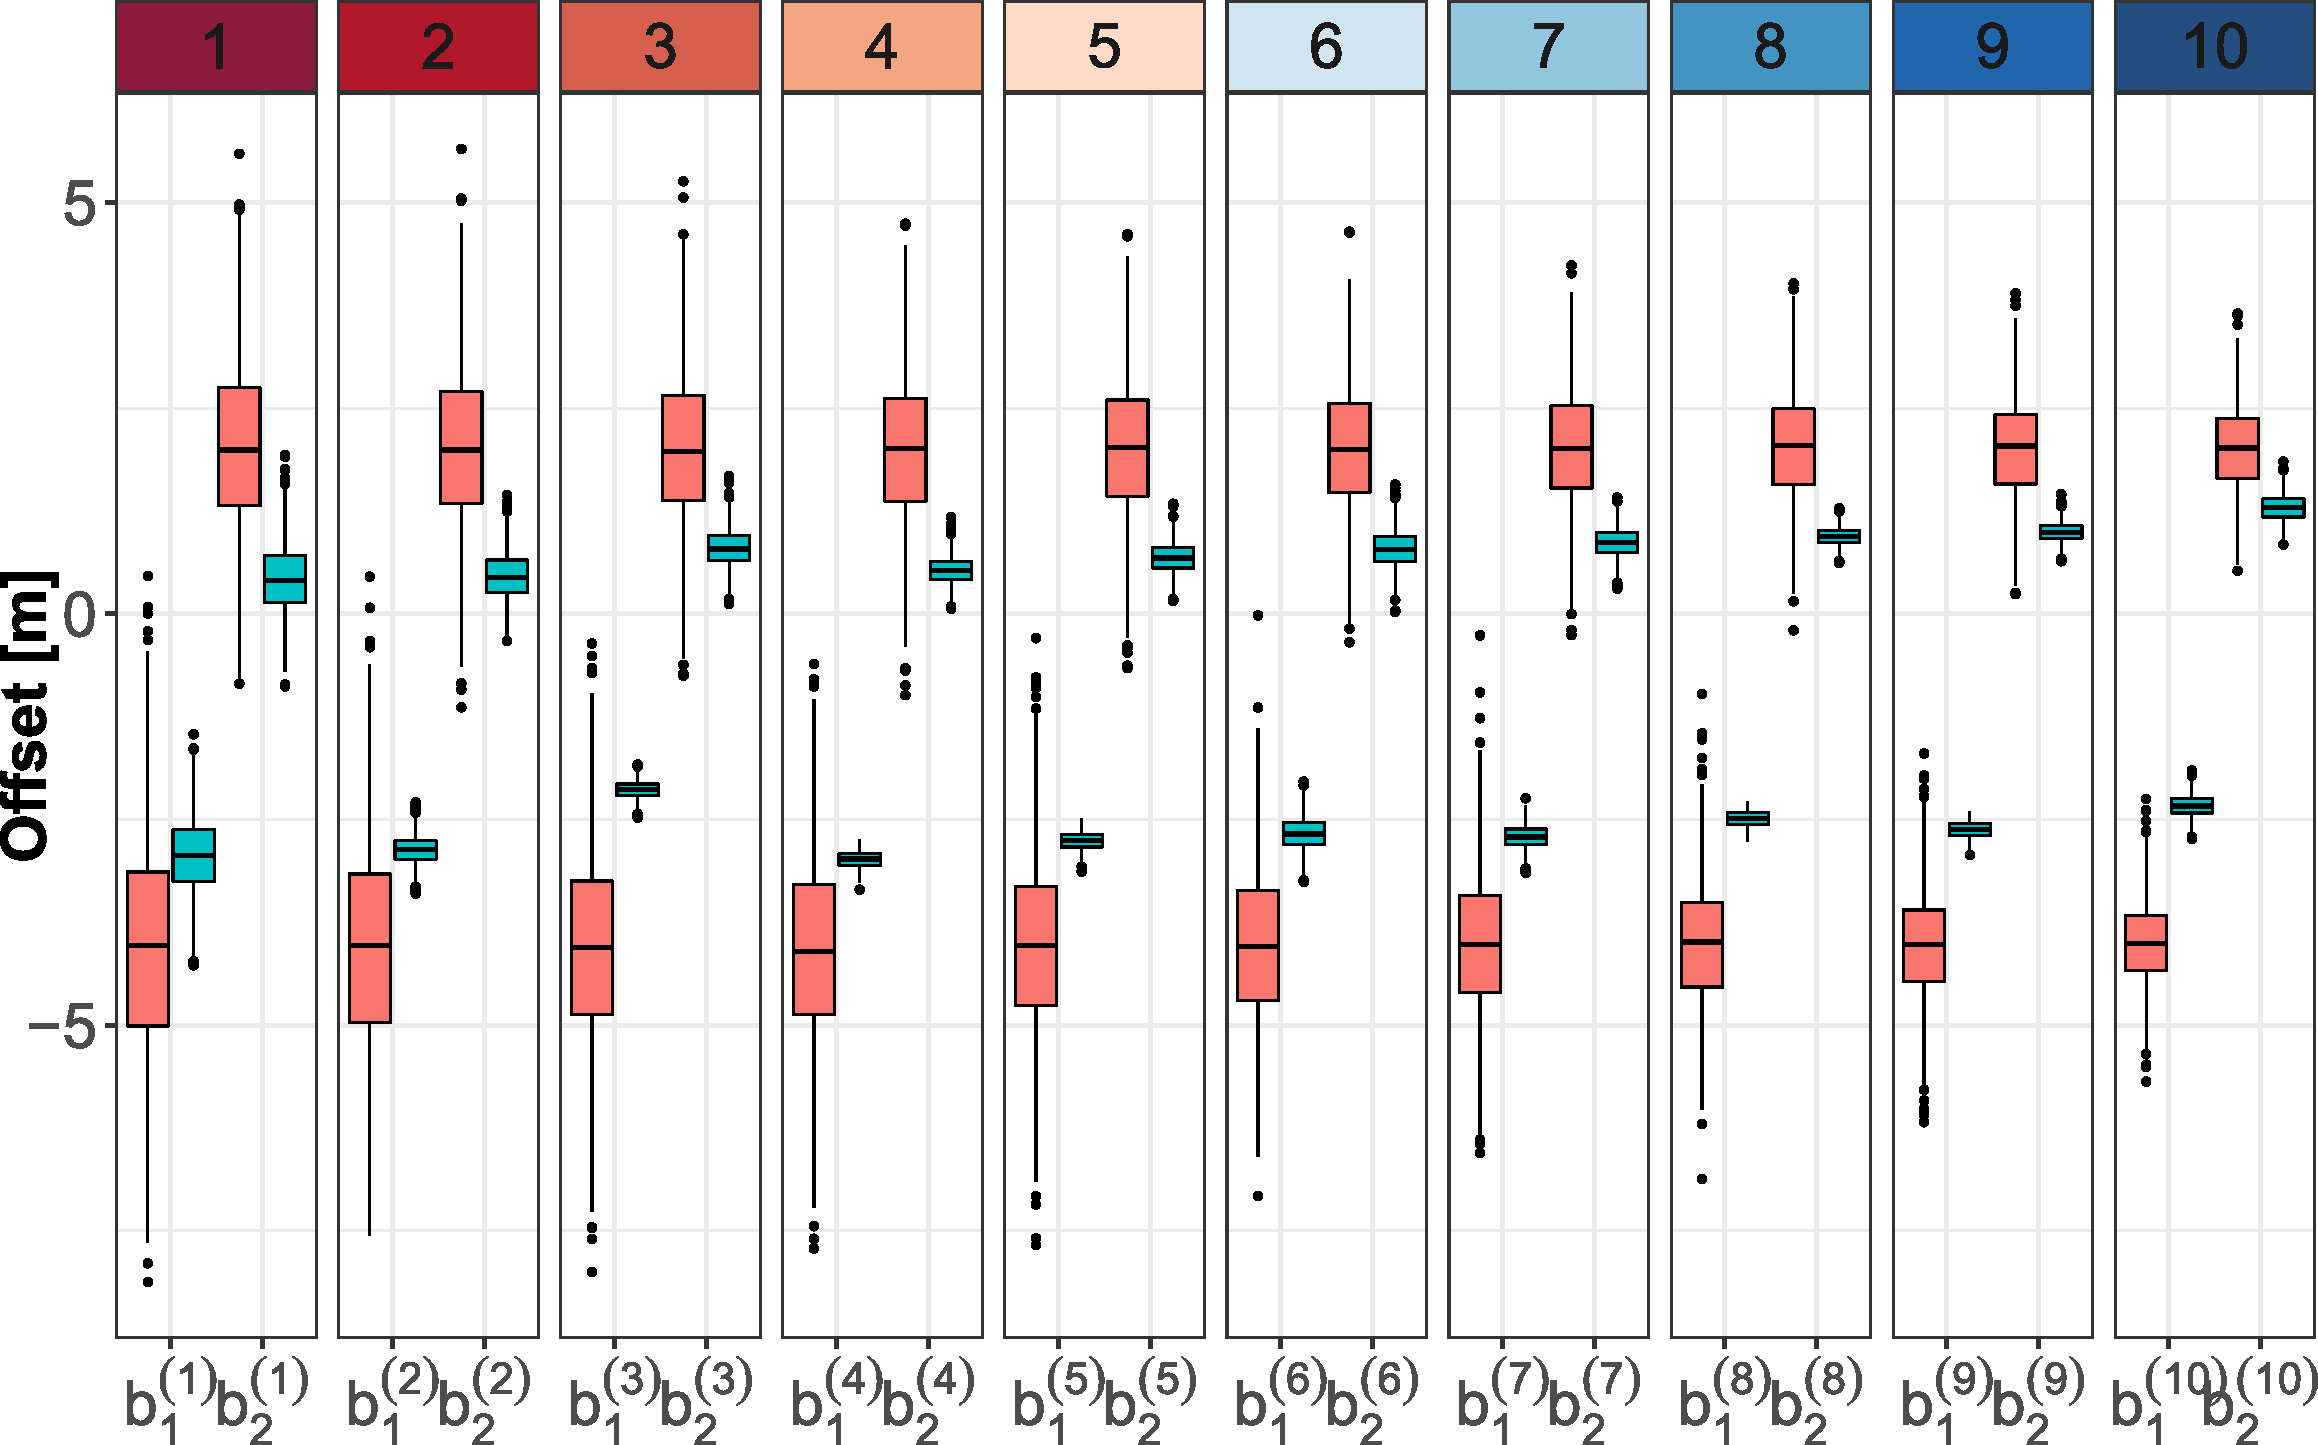
\includegraphics[width=\linewidth]{Chapitre3/Figures/7c-bs_Pt.pdf}
            \caption{}
            \label{subfig:B'sPt}
        \end{subfigure}
        \begin{subfigure}{0.49\textwidth}
            \centering
            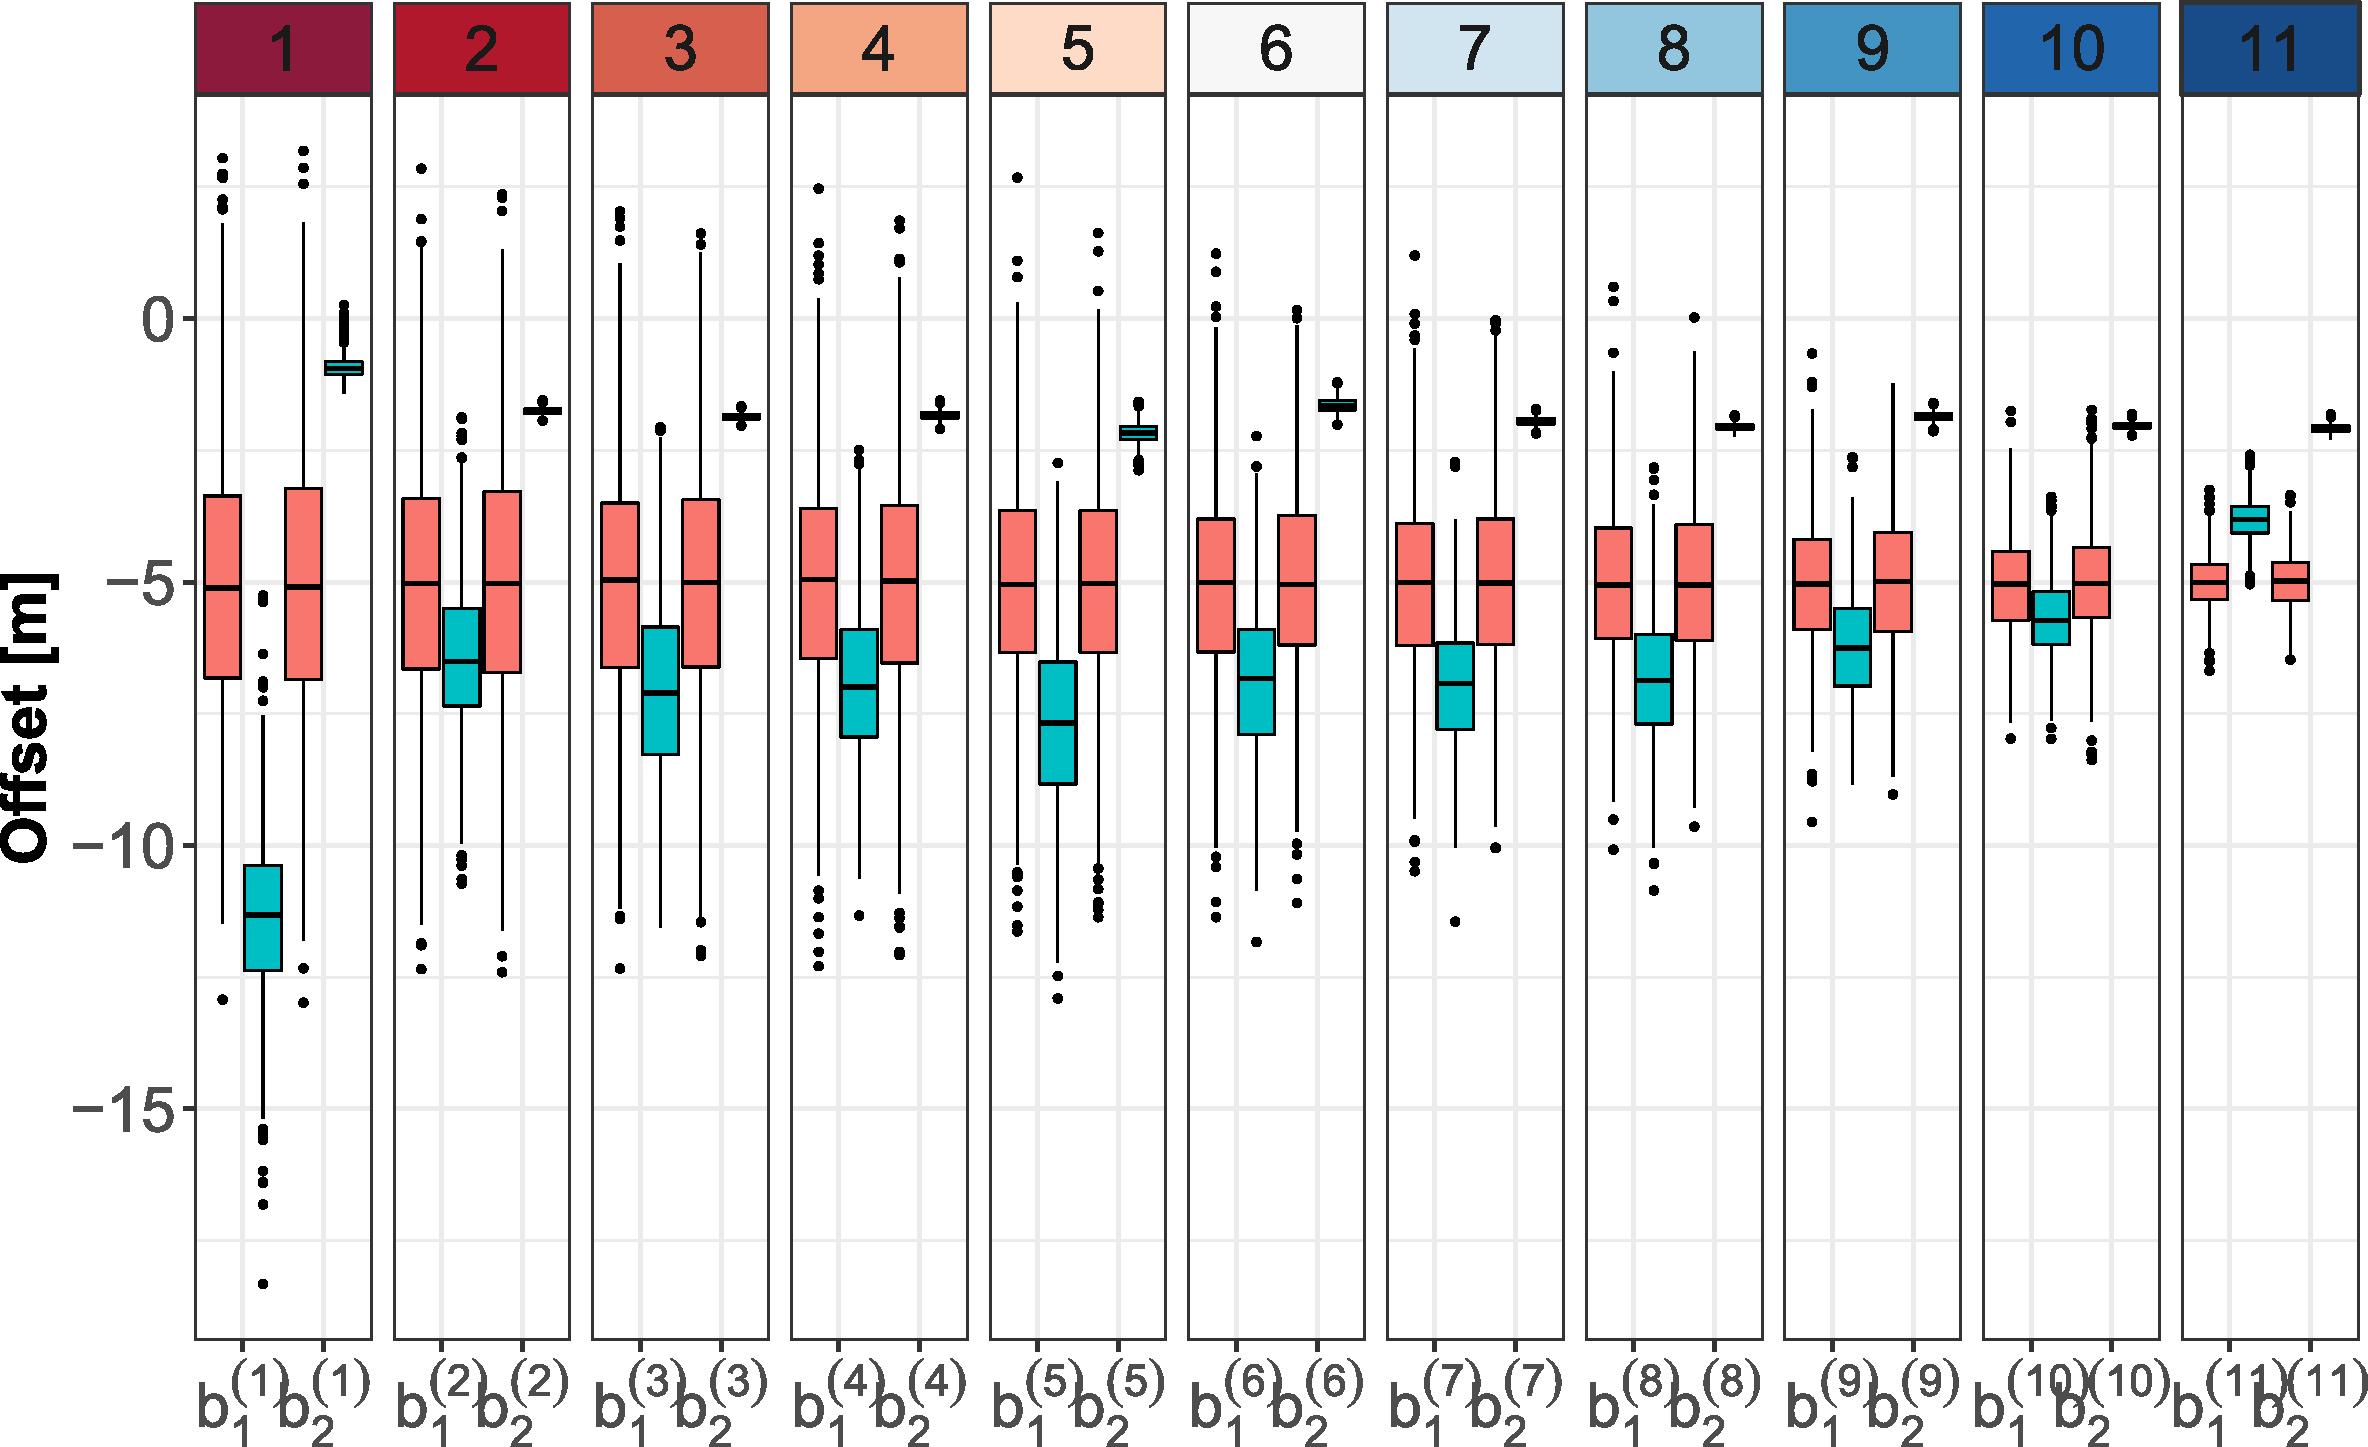
\includegraphics[width=\linewidth]{Chapitre3/Figures/7d-bs_Restit.pdf}
            \caption{}
            \label{subfig:B'sRes}
        \end{subfigure}
        % \caption{Offsets priors and posteriors for Pont de Beaucaire (left) and Beaucaire restitution (right)}
        
        \begin{subfigure}{0.39\textwidth}
            \centering
            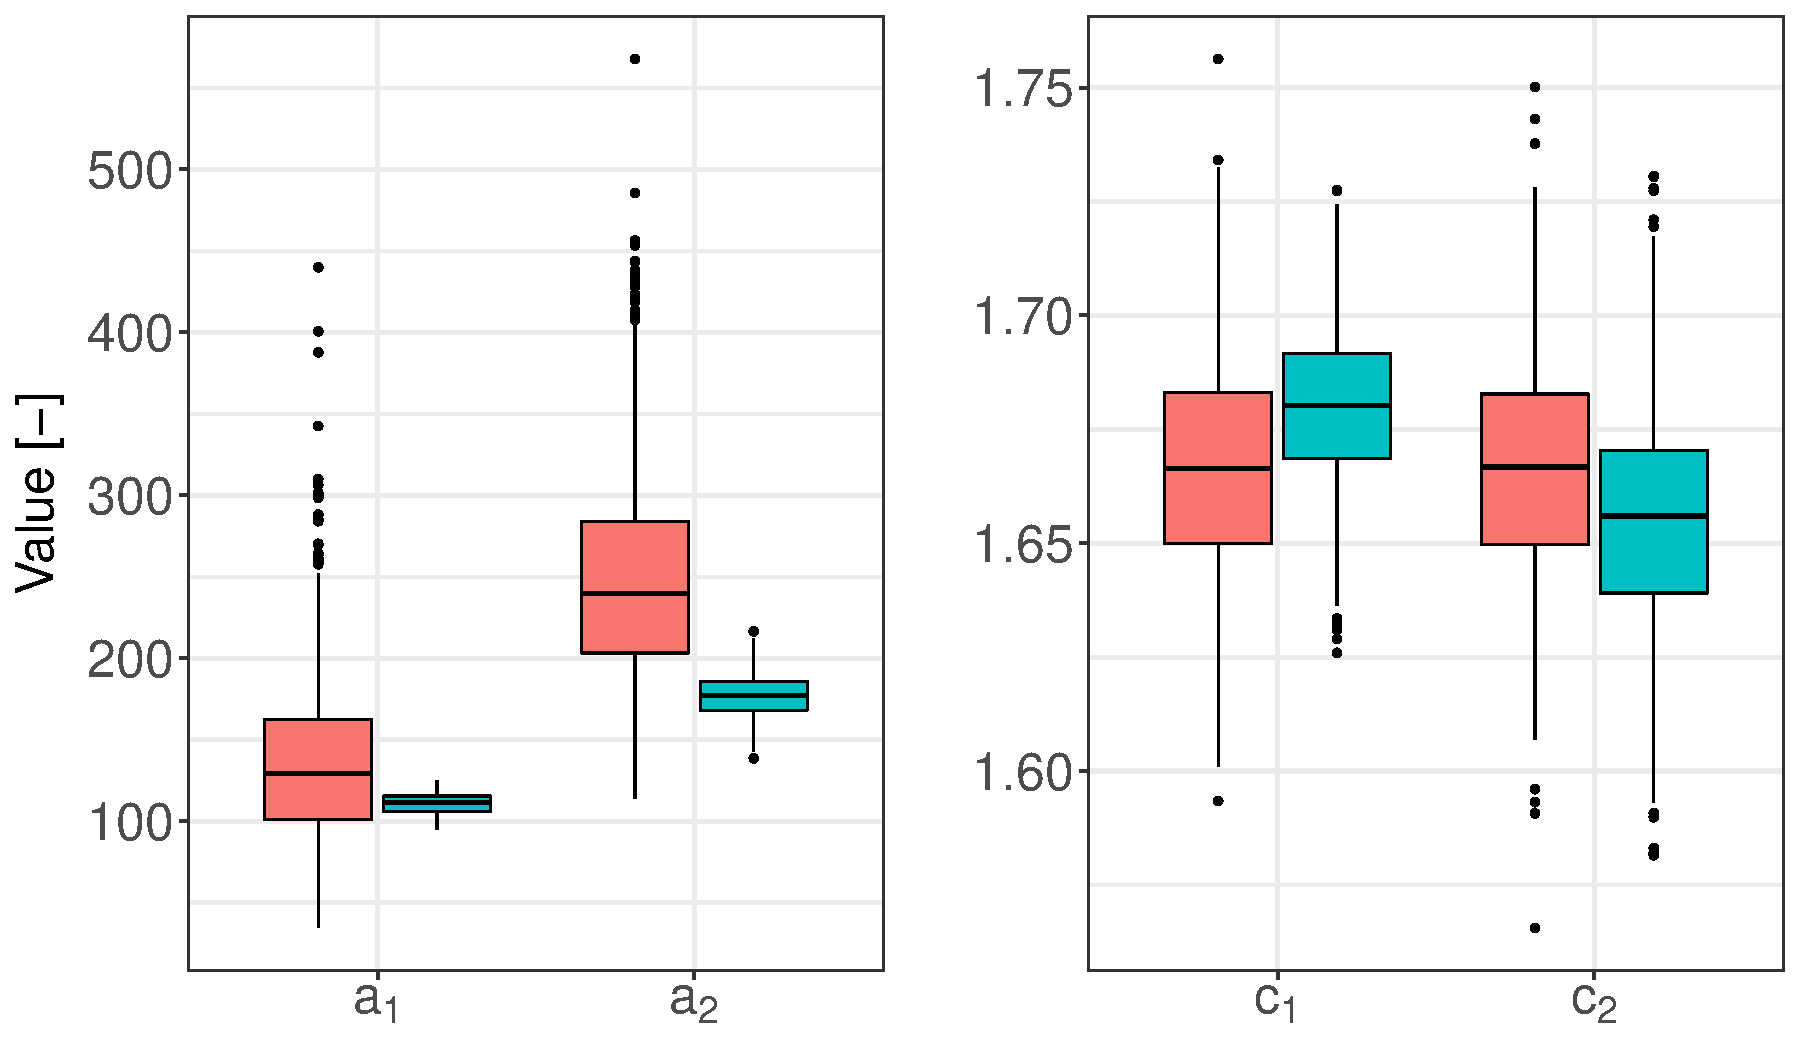
\includegraphics[width=\linewidth]{Chapitre3/Figures/7e-a&csPt.pdf}
            \caption{}
            \label{subfig:a's and c's Pt}
        \end{subfigure}
        \begin{subfigure}{0.49\textwidth}
            \centering
            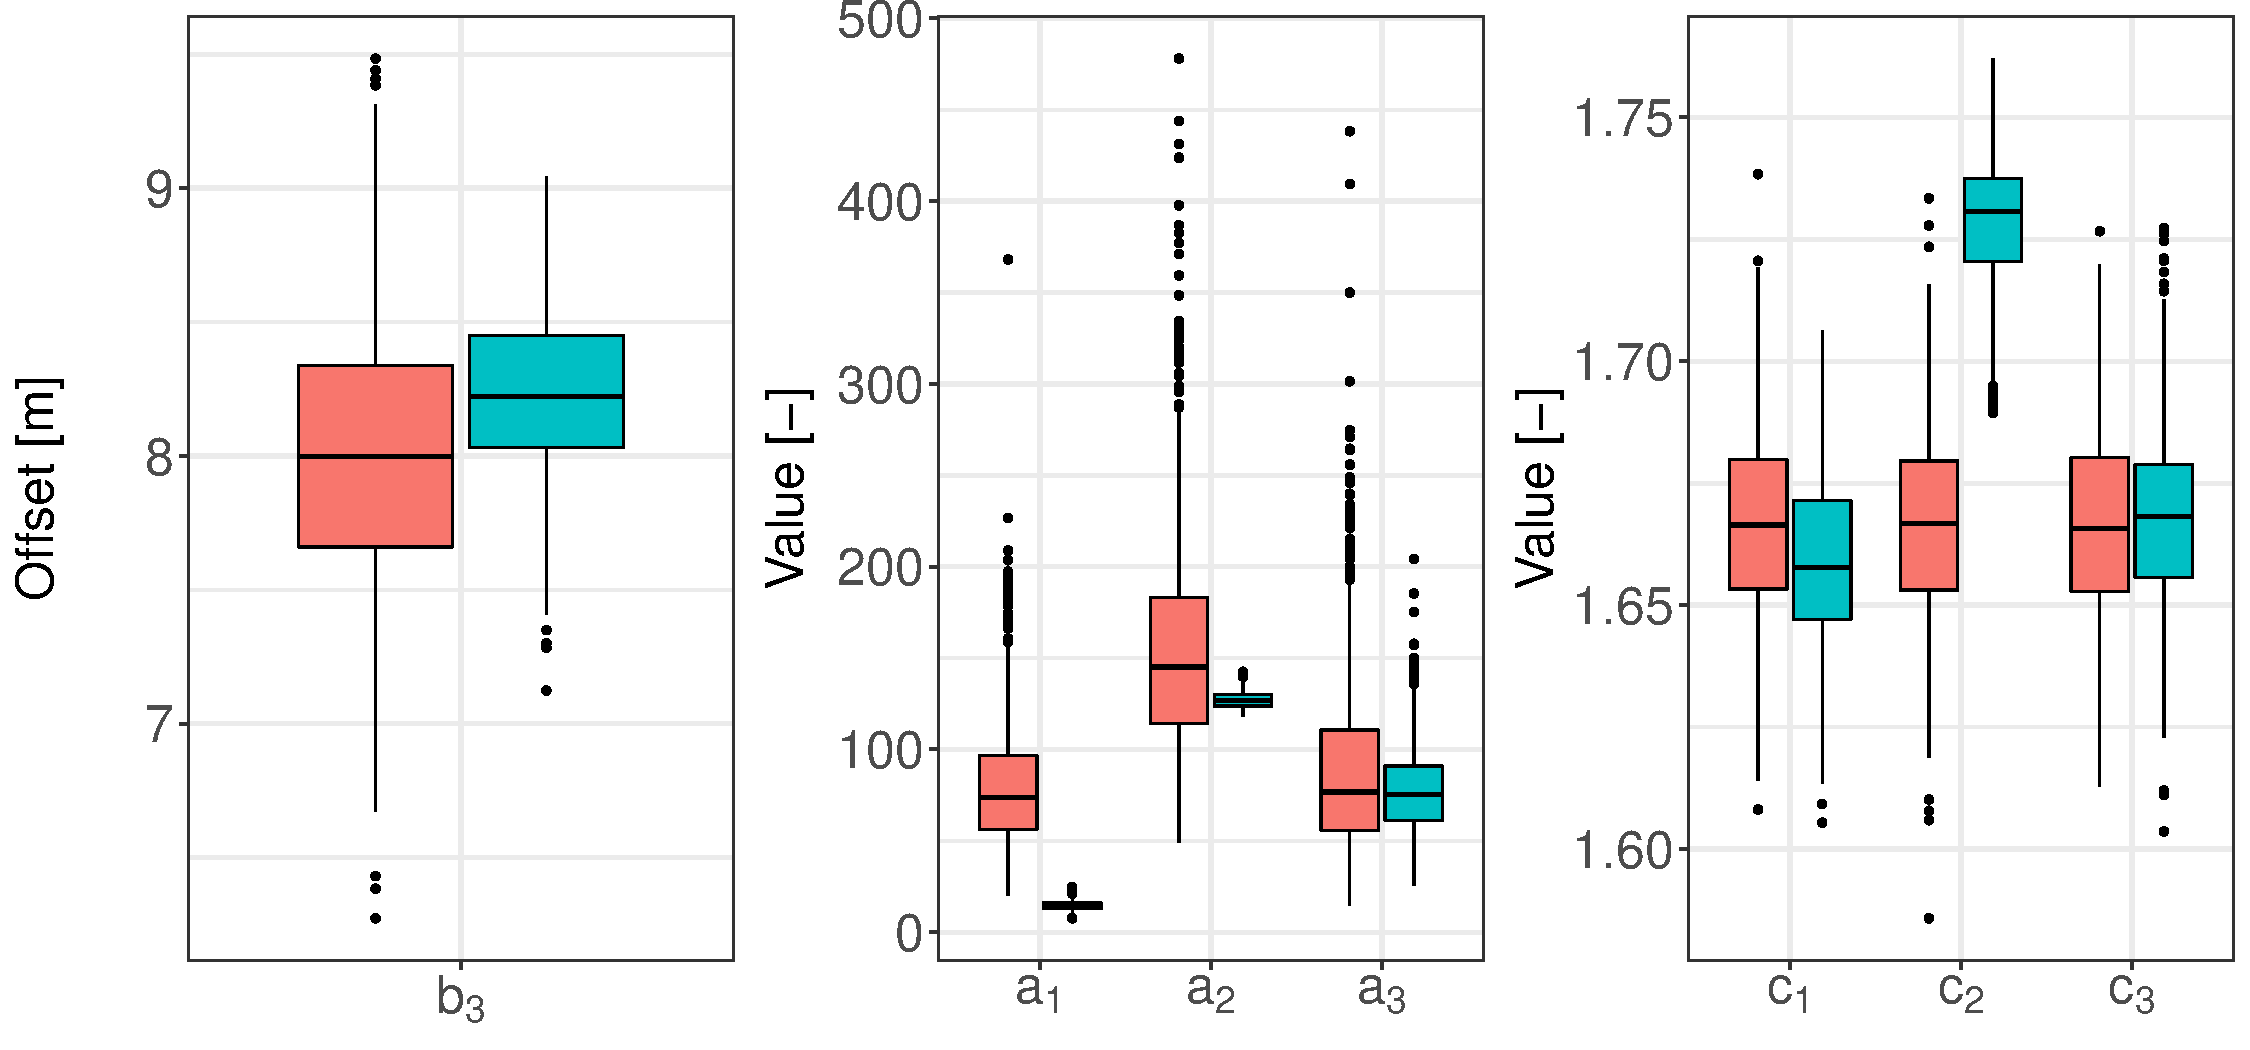
\includegraphics[width=\linewidth]{Chapitre3/Figures/7f-b3_as_cs_Restit.pdf}
            \caption{}
            \label{subfig:bac'sRes}
        \end{subfigure}
        \begin{subfigure}{0.1\textwidth}
            \centering
            \raisebox{2.2cm}{%
            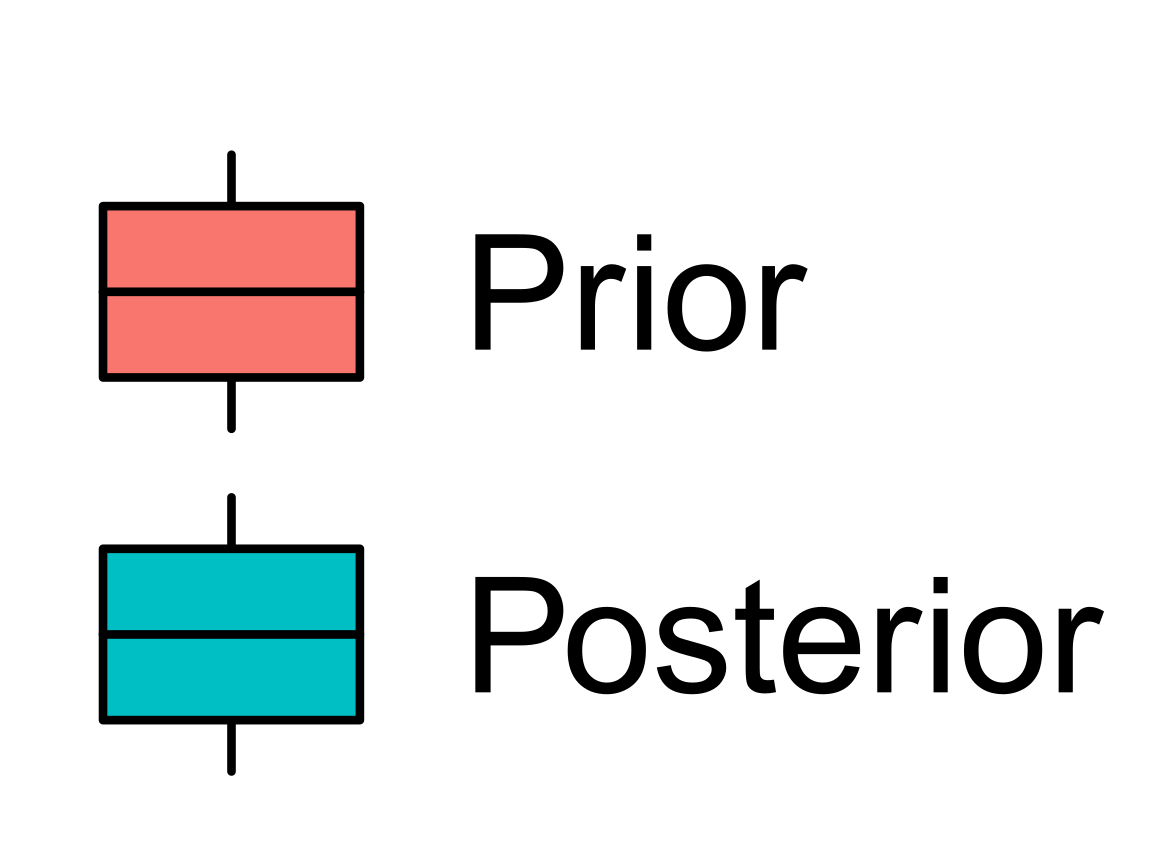
\includegraphics[width=\linewidth]{Chapitre3/Figures/7g-Legend.png}}
        \end{subfigure}
        % \caption{Static parameters priors and posteriors for Pont de Beaucaire (left) and Beaucaire restitution (right)}
        \caption{Pont de Beaucaire (a) and Beaucaire Restitution (b) rating curves and relative 95\% uncertainty with respect to maxpost, offsets priors and posteriors (c and d) and static parameters priors and posteriors (e and f). Discharges of rating curves are in logarithmic scale, solid lines represent maxpost values, grey transparent envelops represent 95\% uncertainty intervals and dots with error bars represent the gaugings with 95\% uncertainty. Stable stage-discharge periods are numbered from the oldest to the latest (see table \ref{tab:ShiftDates}).}
        \label{fig:RcsAndParams}
    \end{figure}
    \FloatBarrier
    
    \subsection{Stage uncertainty}
    \label{subsec:StageErrResults}
    
    The error sources described in table \ref{tab:StageErr} are combined using a Monte Carlo procedure to quantify the uncertainty affecting AMAX stages as described in figure \ref{fig:StageErrAMAX}. The measured stage is outside and below the stage uncertainty interval before 1840 at Pont de Beaucaire: this is due to the exponential distribution used to model measurement frequency errors which are dominant during this period and are positive by definition. The upper uncertainty bound is sometimes 1.5 meters higher than the measured stage. Therefore, considering this source of uncertainty may have substantial consequences on the final results. The difference between uncertainty bounds and originally measured stages is presented in the bottom part of figure \ref{fig:StageErrAMAX}. The uncertainty of AMAX stages decreases over time as the measurement frequency and precision improve. The width of the 95\% uncertainty interval is 1.7 m before 1840, 0.3 m between 1840 and 1967, and 0.24 m at Beaucaire Restitution (1970-2020). The 5 m threshold above which hourly measurements were done after 1840 explains the large reduction of the uncertainty. After 1840, the uncertainty is controlled by the exceedance of this 5 m threshold, the AMAX below 5 m being penalized by non-negligible measurement frequency errors $\delta_5$. 
    
    \begin{figure}[h!]
        \centering
        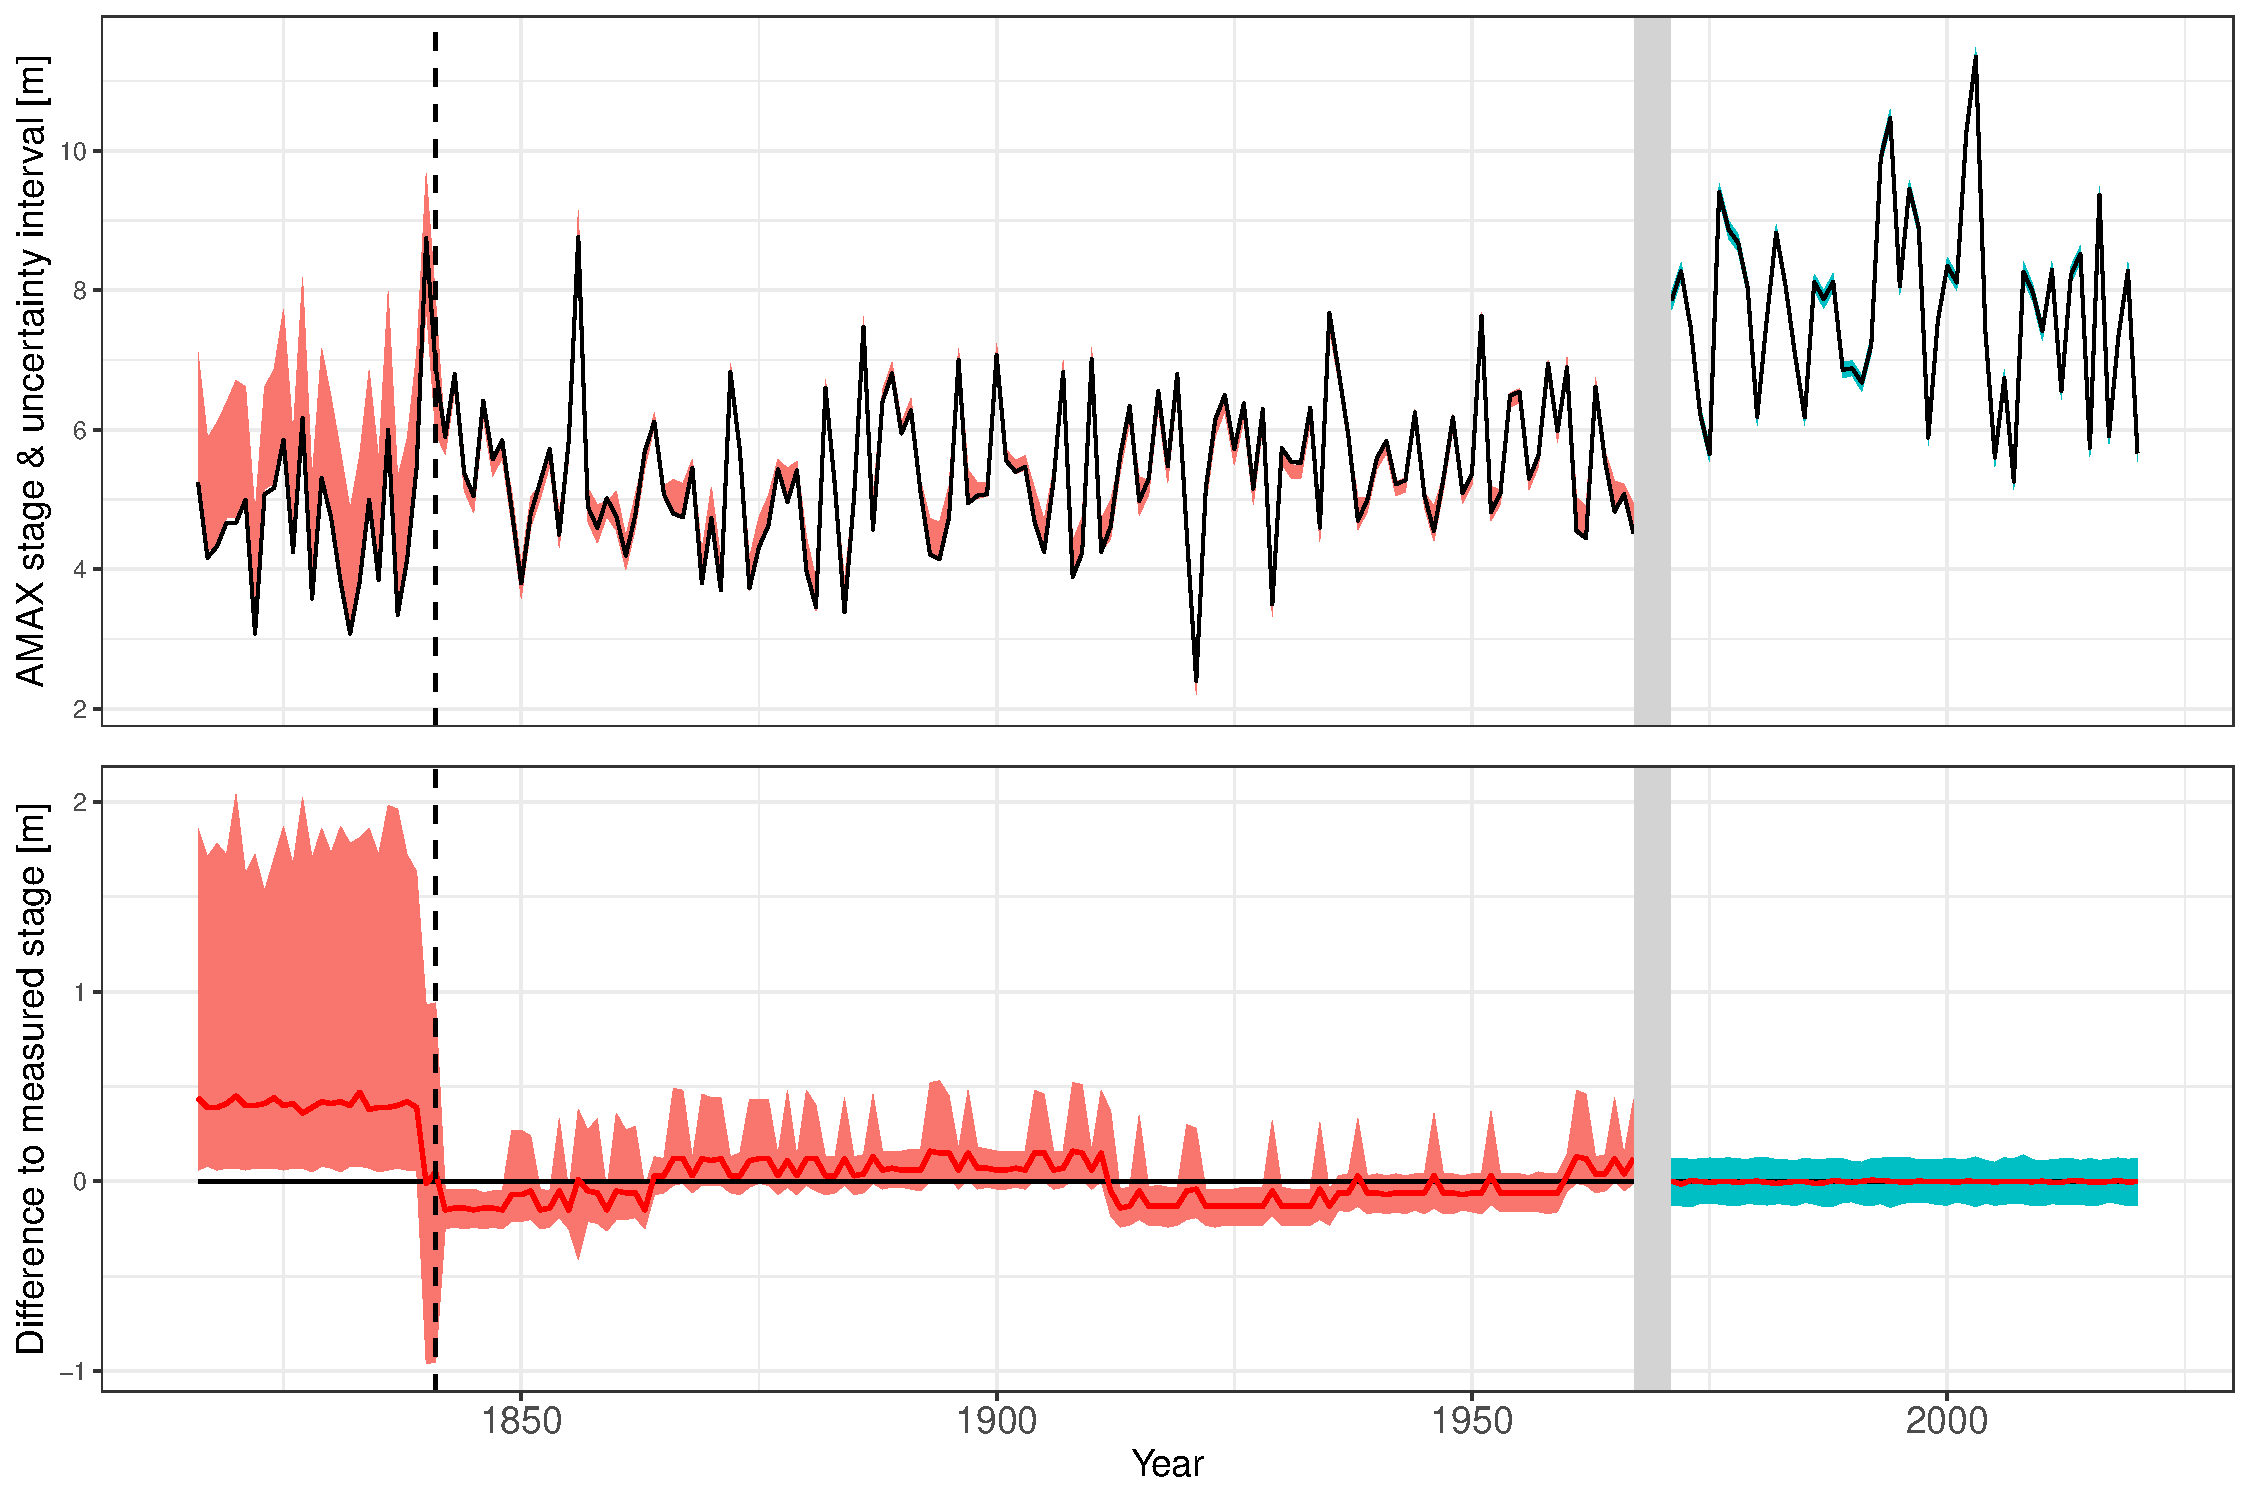
\includegraphics[width=0.9\linewidth]{Chapitre3/Figures/8-StageErrorAMAX_BOTH.pdf}\hfill
        \caption{Top: AMAX stages and uncertainty at Beaucaire (1816-2020). Bottom: Difference between 95\% stage uncertainty bounds and originally measured stage.}
        \label{fig:StageErrAMAX}
    \end{figure}
  \FloatBarrier

    \subsection{Total streamflow uncertainties}
    
    \paragraph{}
    Stage uncertainties are propagated through uncertain rating curves as described in section \ref{subsec:PropagStage} and the results are shown in figure \ref{fig:ICtot_both}. Streamflow uncertainty, although fluctuating, decreases over time from 30\% before 1840, and 10\% before 1967, to 5\% at Beaucaire Restitution (1967-2020). This 5\% uncertainty on recent AMAX discharges is consistent with the results of the international consensus conference on the December 2003 flood : “The most likely estimate of the maximum discharge of the Rhône River at Beaucaire during the December 2003 flood is 11500 m3/s, corresponding to a return period slightly above 100 years. […] This maximum discharge estimate is subject to an uncertainty of around 5\%, resulting from the uncertainty of flow measurements, maximum stage, parameterization and extrapolation of the December 2003 gauging data.” \citep{medd_debit_2005}.
    
    \paragraph{} Stage uncertainty appears dominant at Pont de Beaucaire, as well as rating curve parametric uncertainty, originating from the difficulty to estimate rating curve parameters with only a few gaugings. Thus, parametric uncertainty is reduced for properly gauged periods. During the Vallabrègues hydraulic system construction (1967 - 1970), the waters of the Durance River, one of the major tributaries, were deviated from the Rhône River course. AMAX discharges of these missing years were reconstructed by CNR with upstream gauging stations. The uncertainty around these reconstructed discharges is assumed to be represented by a Gaussian distribution with 10\% relative standard deviation. An AMAX flow (with uncertainties) time series plot is available in supplementary material (figure 3).
    
    \begin{figure}[h!]
        \centering
        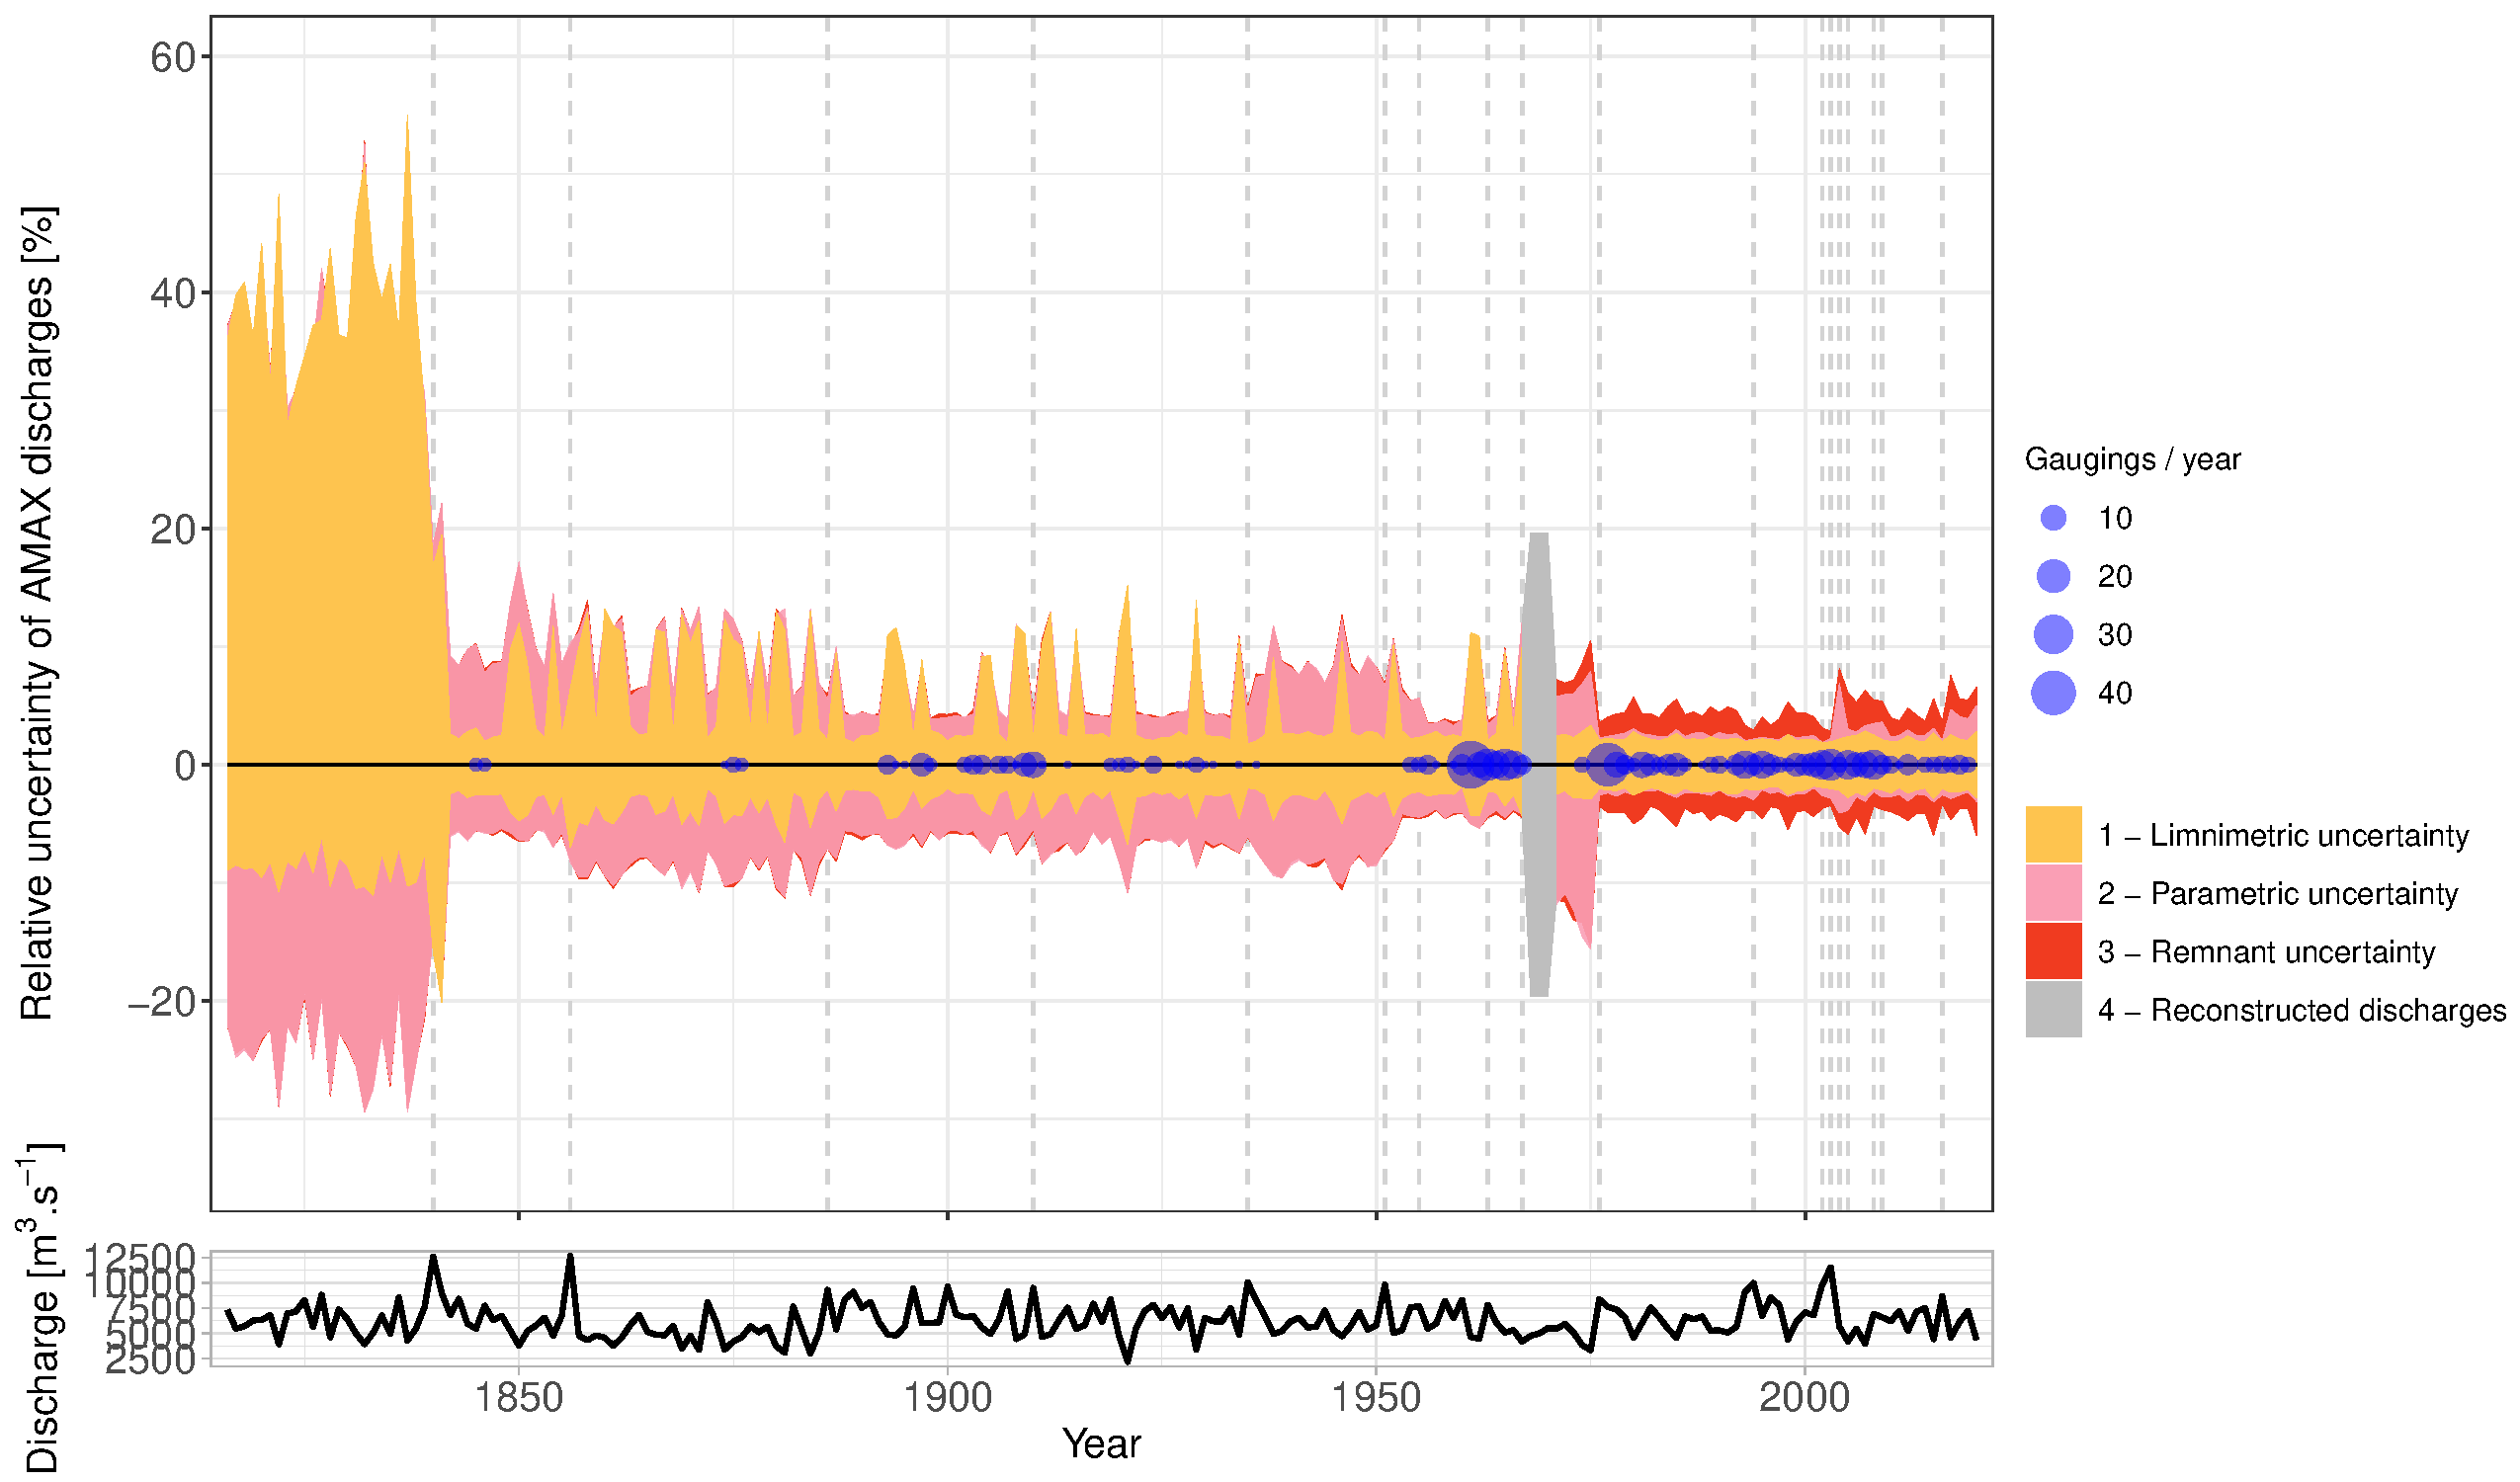
\includegraphics[width=\textwidth]{Chapitre3/Figures/9-IcAndAMAX.pdf}
        \caption{Relative 95\% uncertainty of AMAX discharges with respect to the maxpost discharges (black solid line) for the three sources of streamflow uncertainties, at Beaucaire (1816 - 2020). Vertical dotted lines represent rating shifts.}
        \label{fig:ICtot_both}
    \end{figure}
    \FloatBarrier
   
    \subsection{Flood frequency analysis}
    
        \subsubsection{Streamflow series homogeneity}
           
        \paragraph{}
        The homogeneity of streamflow series is an essential prerequisite as FFA is based on the hypothesis of iid (independent and identically distributed) random variables. In order to check this hypothesis, the Mann-Kendall non-parametric test (\citet{mann_nonparametric_1945}; \citet{kendall_rank_1948}) is applied to AMAX series at Beaucaire. As streamflow uncertainty is represented by 500 AMAX discharge realizations (section \ref{subsec:PropagStage}), the homogeneity test is applied to each of the 500 AMAX series. Among the Mann-Kendall tests, 81\% concluded to the non-rejection of the null hypothesis (there is no trend in the series) with a 0.05 significance level. We assume that this is enough to consider the series as homogeneous and to proceed to FFA. 
        
        \subsubsection{Flood frequency analysis}
        
       The GEV distribution estimation procedure described in section \ref{subsec:FFA} is applied to the 205-year long AMAX discharges series at Beaucaire accounting for uncertainties. Vague priors are used for GEV parameters: flat priors for location and scale parameters, and Gaussian with zero mean and 0.2 standard deviation for the shape parameter. This shape parameter prior is consistent with \citet{martins_generalized_2000} suggestions.
       Flood quantiles results (figure \ref{subfig:GEV205y}) show that streamflow uncertainty dominates for the lowest return periods, but sampling uncertainty becomes dominant when the return period tends toward 1000 years (see figure \ref{subfig:UKplot4cases} bottom right  for a better understanding of the respective part of each source of uncertainty in this 205 years case). The observed AMAX discharges display a large variability of streamflow uncertainties. The three largest floods of this 205 years sample (1840, 1856 and 2003, by chronological order and from the most uncertain to the most precise) illustrate this point. Thus, not considering 1840 and 1856 floods could have a strong effect on the estimation of the maxpost quantiles values, as well as their uncertainty. This is explored next by varying the sample size.
       
       % \begin{figure}[h!]
       %      \centering
       %      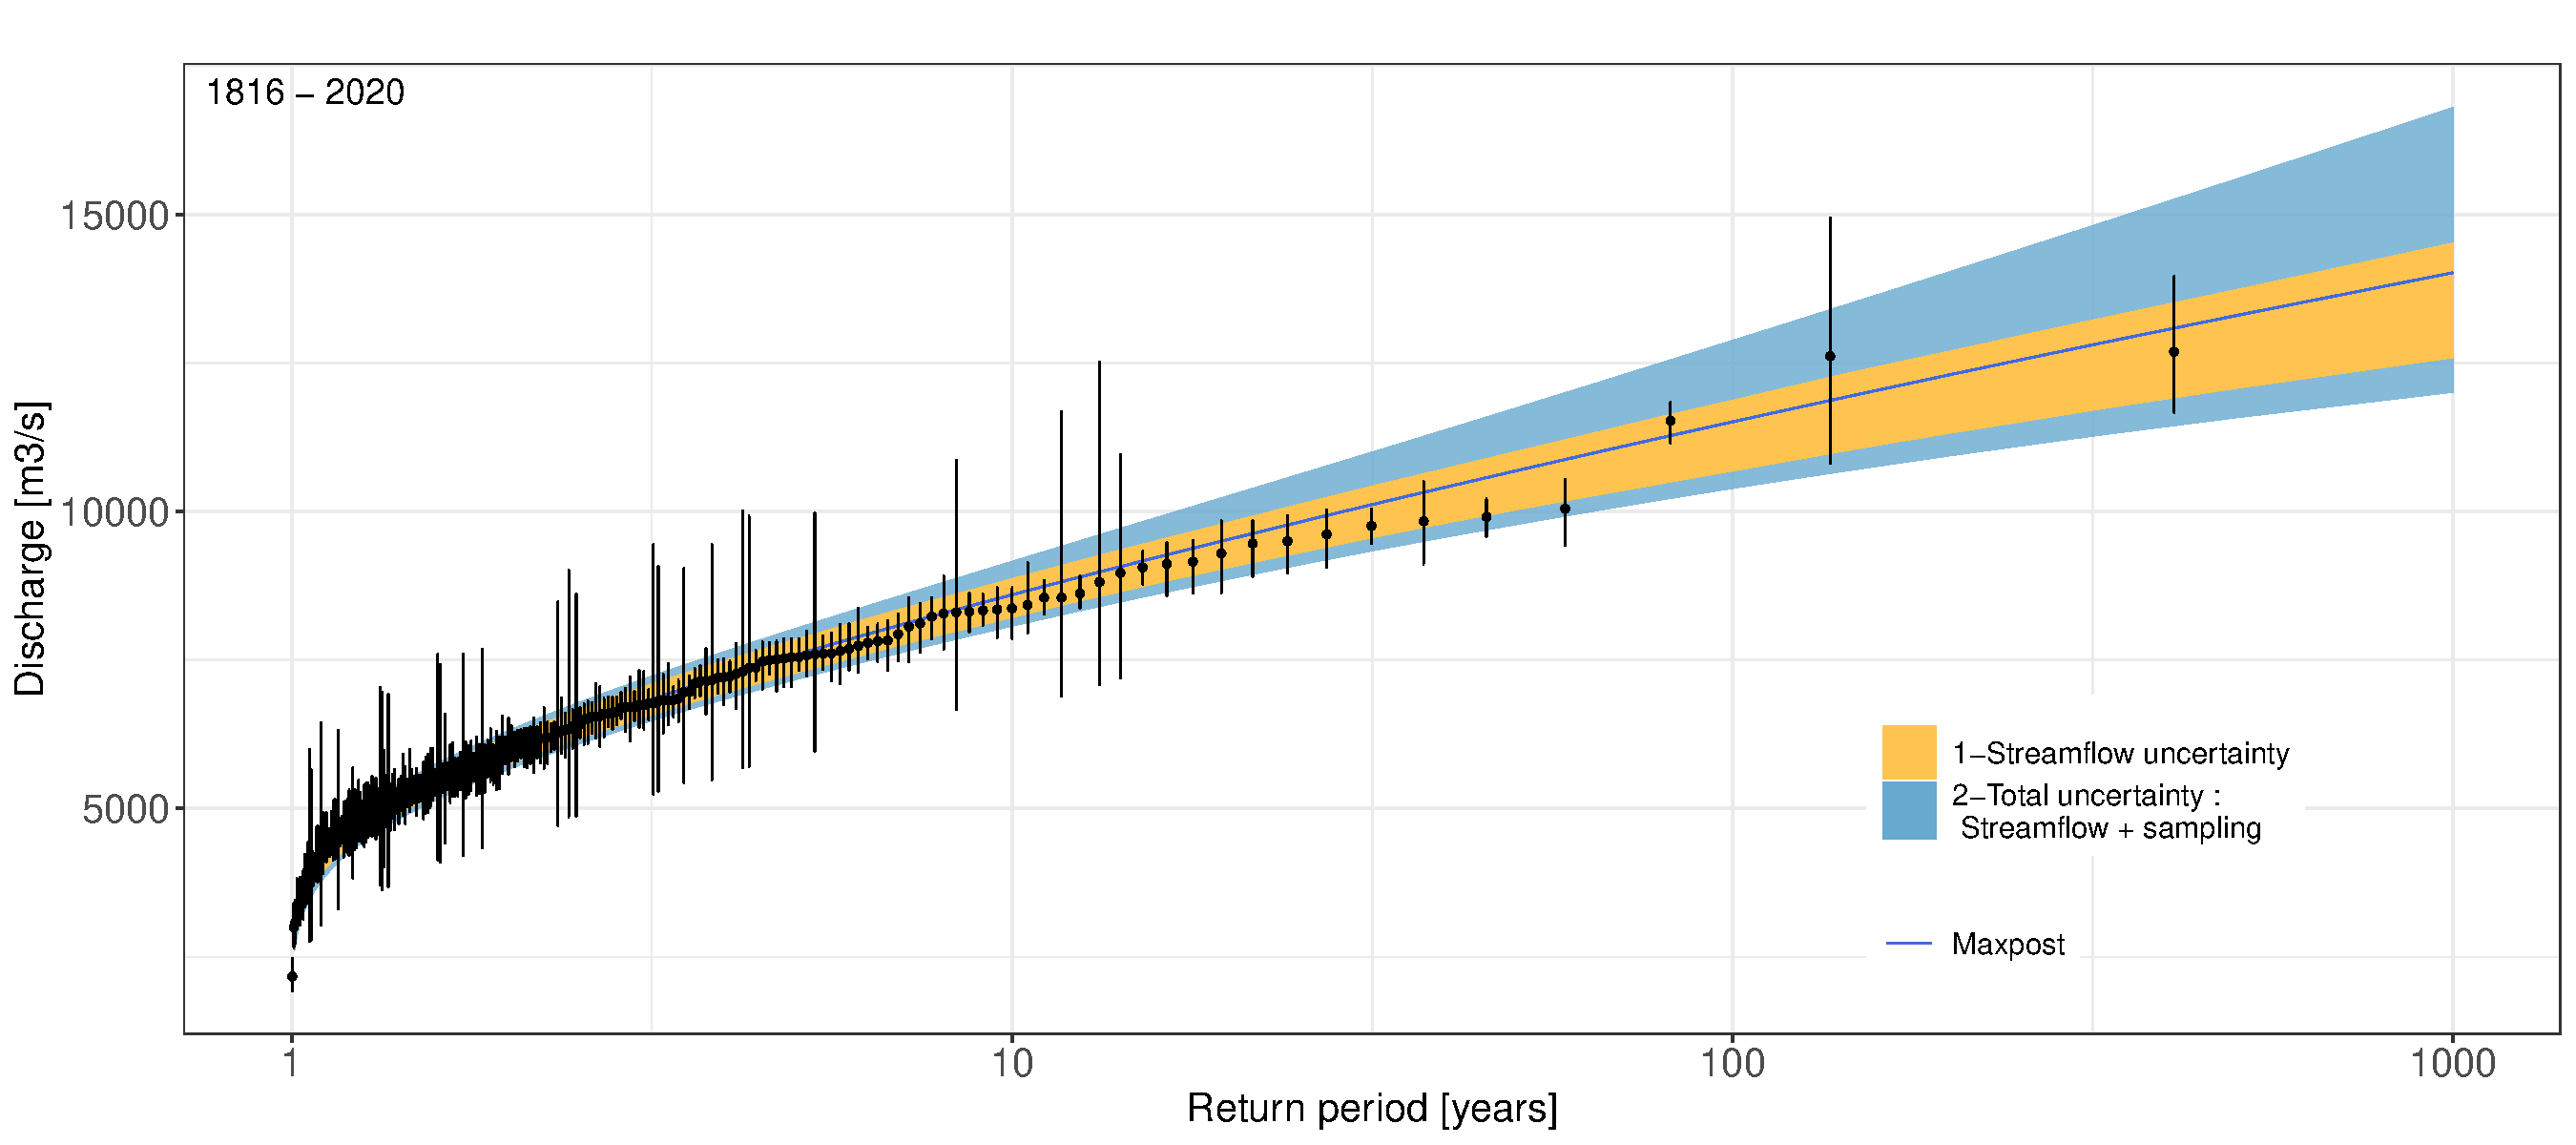
\includegraphics[width=0.7\linewidth]{Figs/10-GeV_205years.pdf}
       %      \caption{Flood quantiles 95\% uncertainty interval for both streamflow and total (streamflow + sampling) uncertainties. Error bars represent the AMAX observed discharges with 95\% streamflow uncertainty.}
       %      \label{fig:GEV205y}
       %  \end{figure}            
        
        \begin{figure}[p]
            \centering
            \begin{subfigure}{0.99\textwidth}
                \centering
                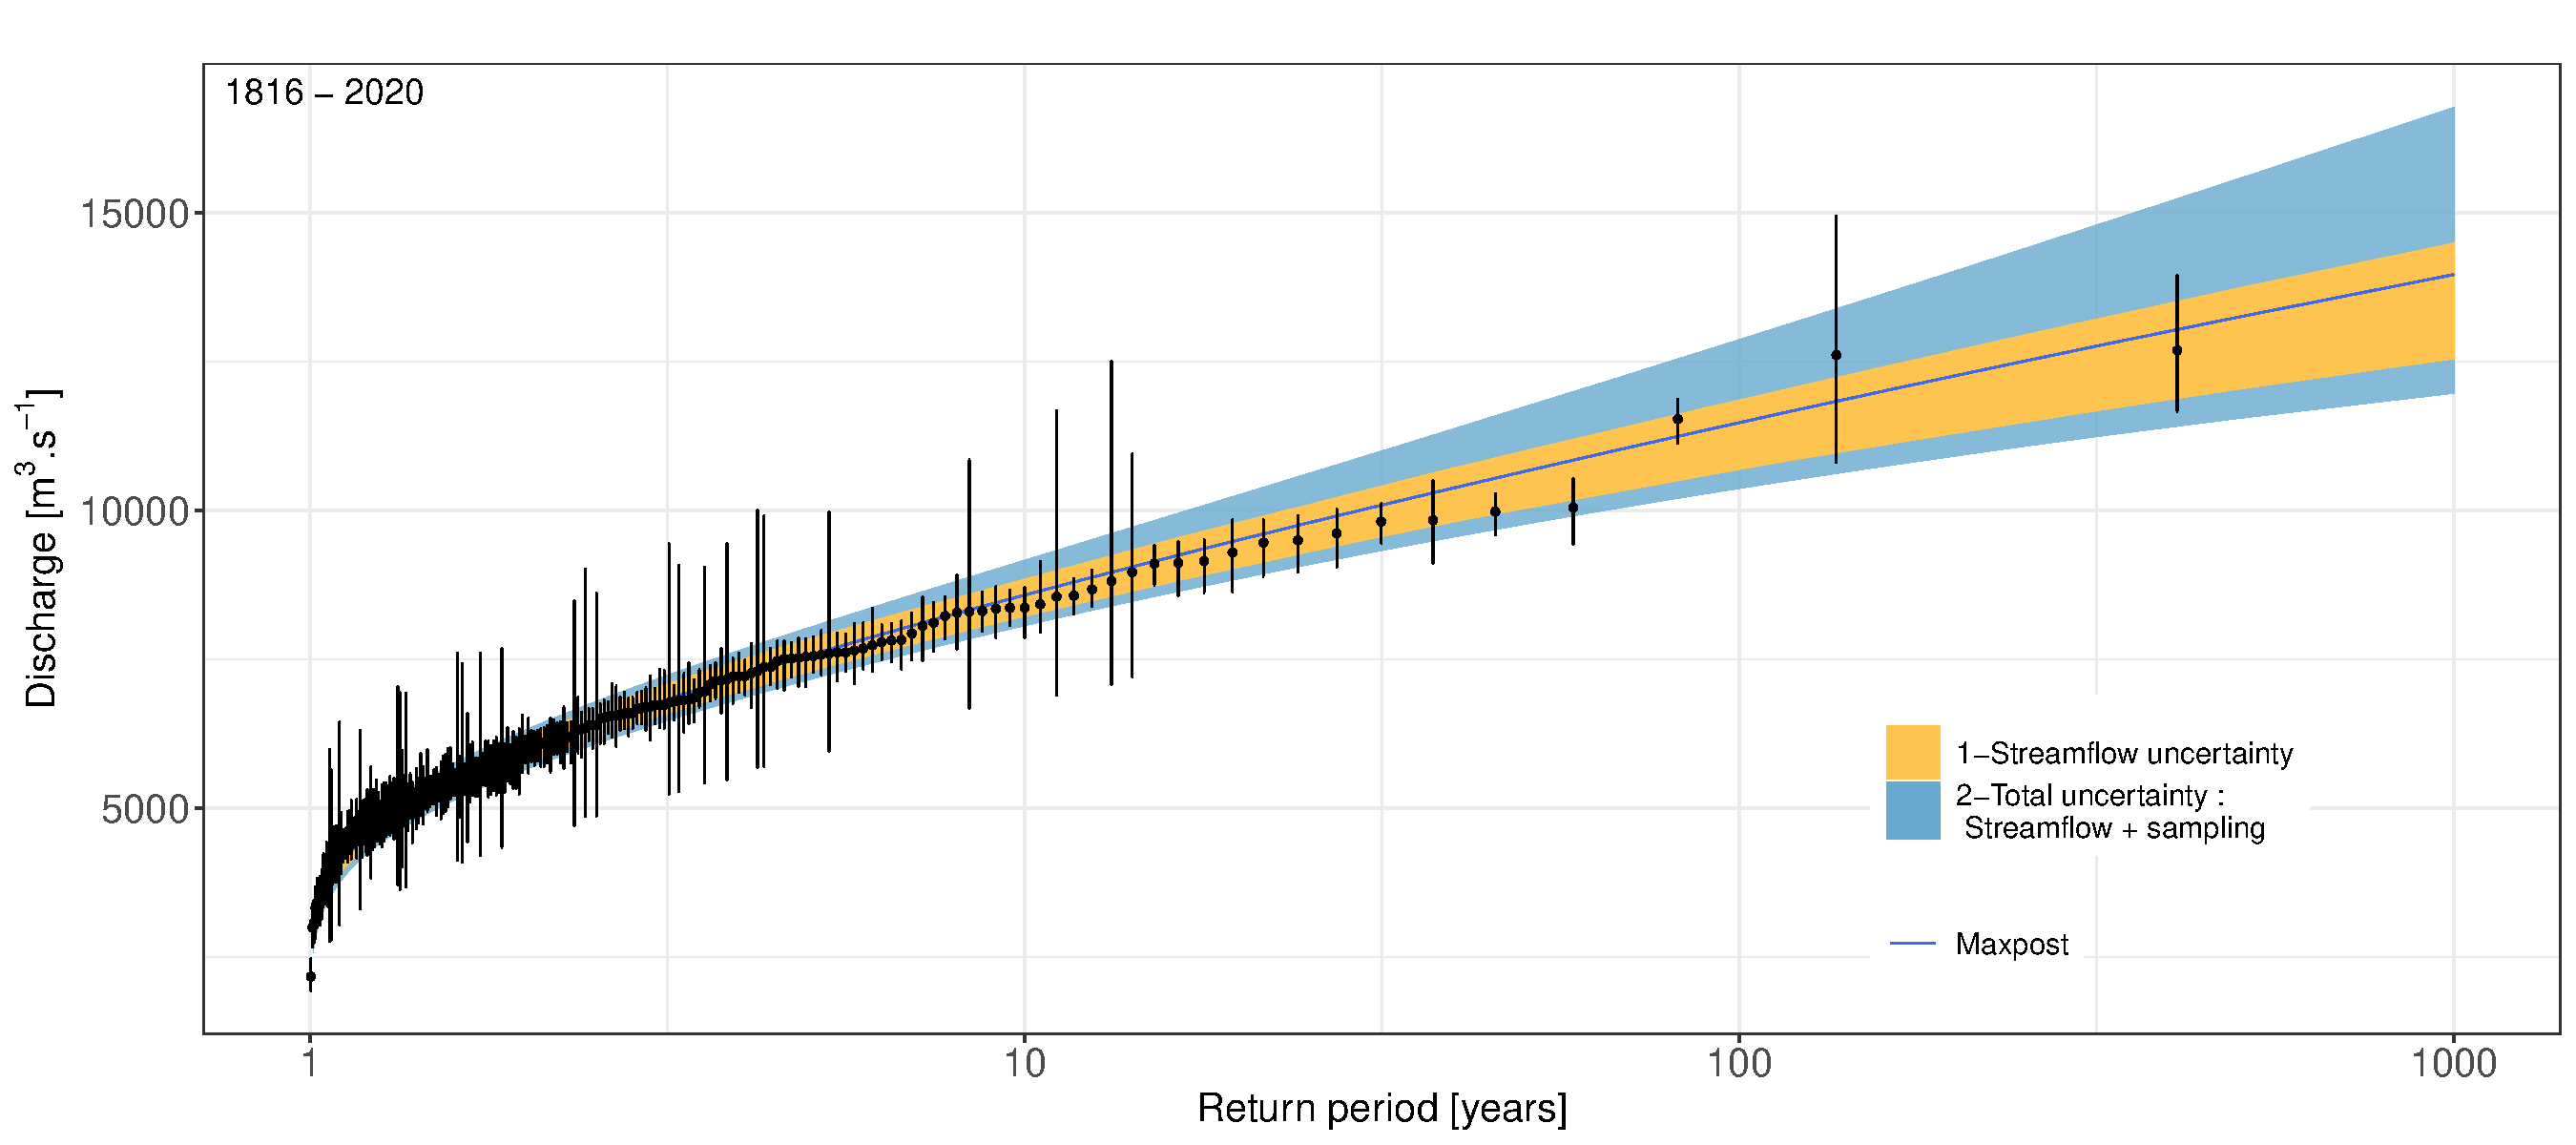
\includegraphics[width=1\linewidth]{Chapitre3/Figures/10a-GeV_205years.pdf}
                \caption{}
                \label{subfig:GEV205y}
            \end{subfigure}
            
            \centering
            \begin{subfigure}{0.49\linewidth}
                \centering
                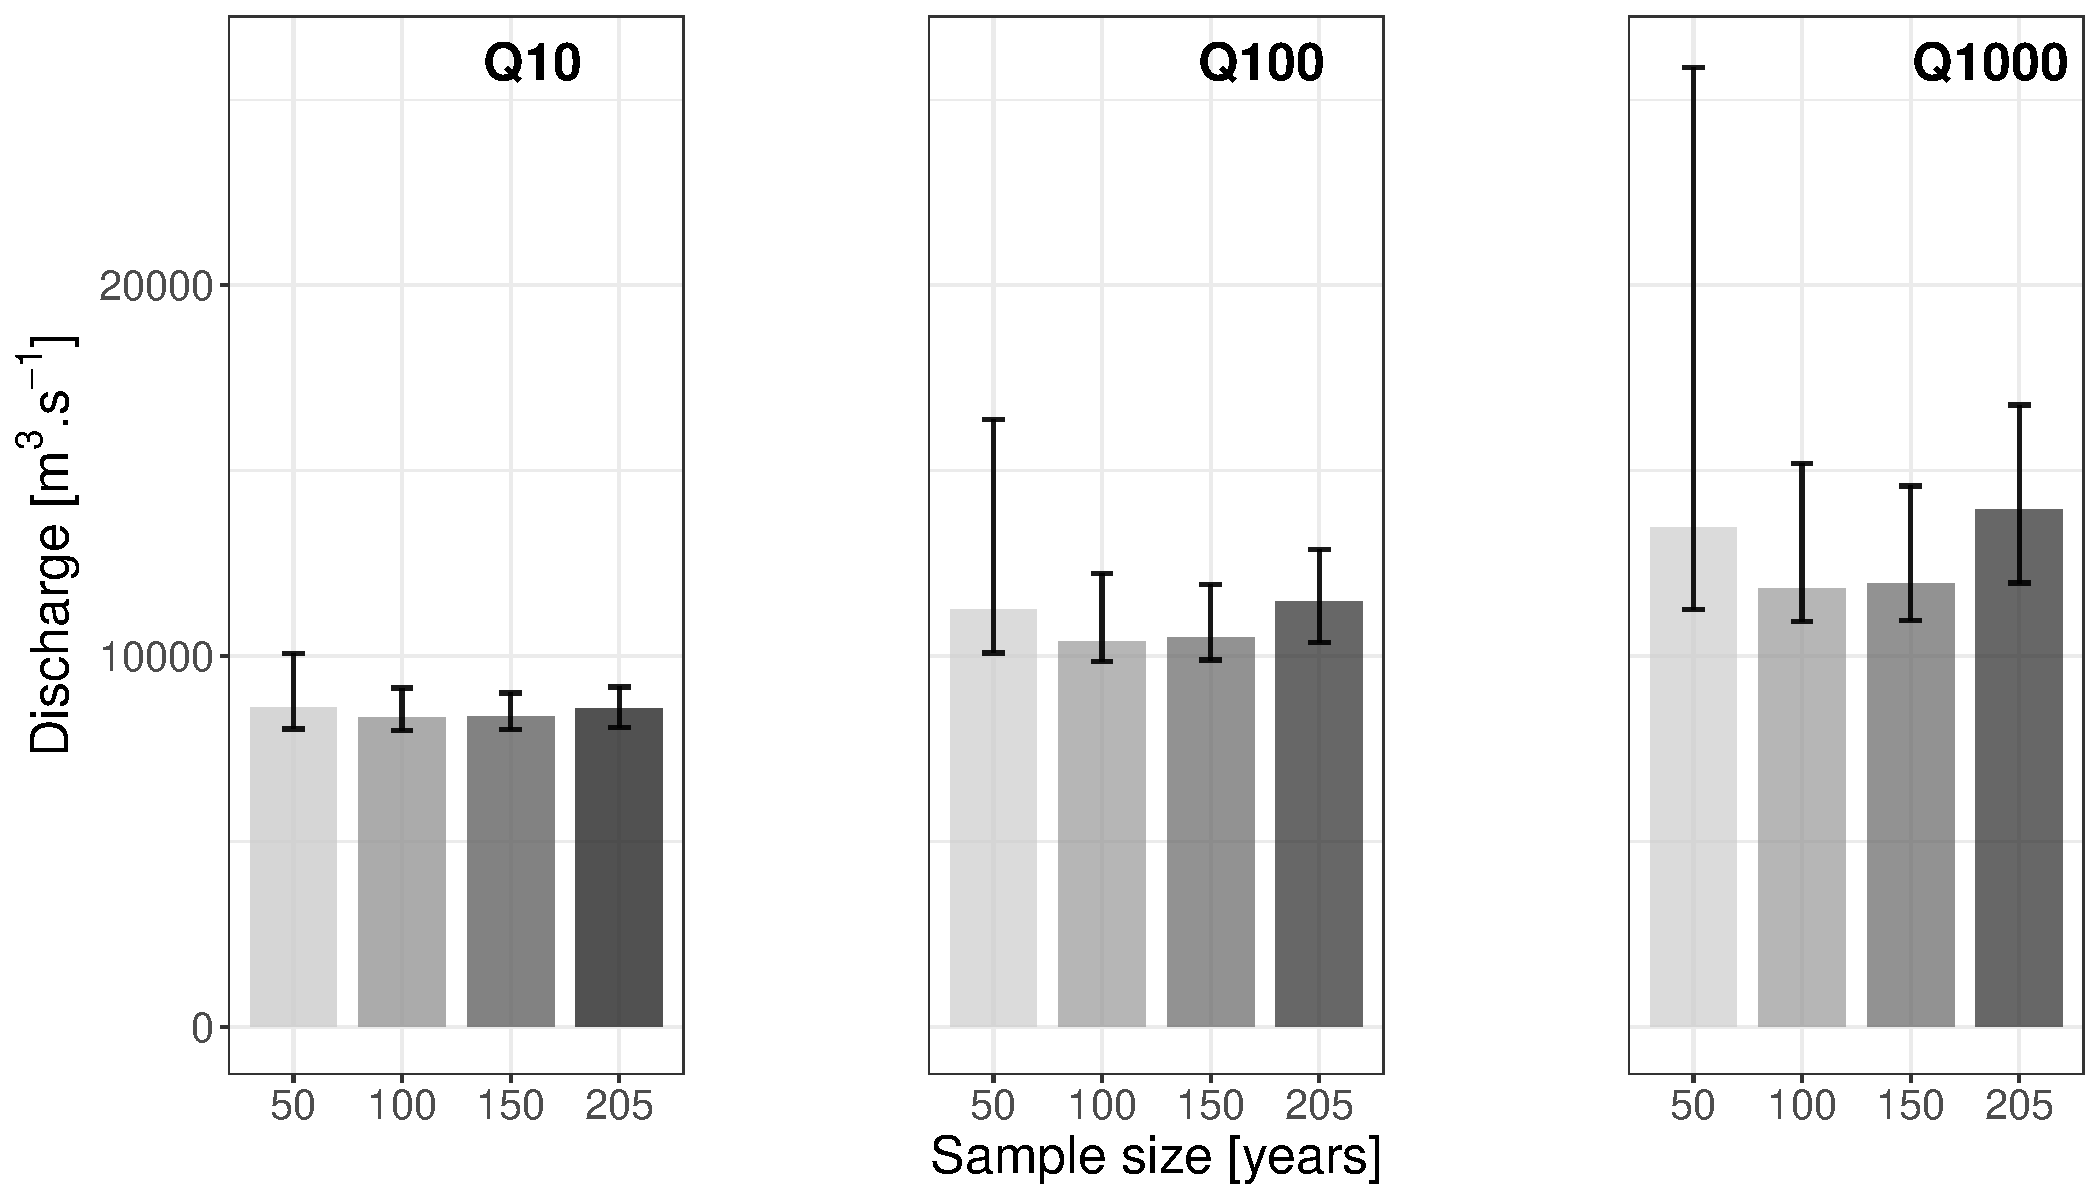
\includegraphics[width=1\linewidth]{Chapitre3/Figures/10b-BarplotQuantiles4cases.pdf}
                \caption{}
                \label{subfig:BarplotQuantilesGev}
            \end{subfigure}
            \begin{subfigure}{.49\textwidth}
                \centering  
                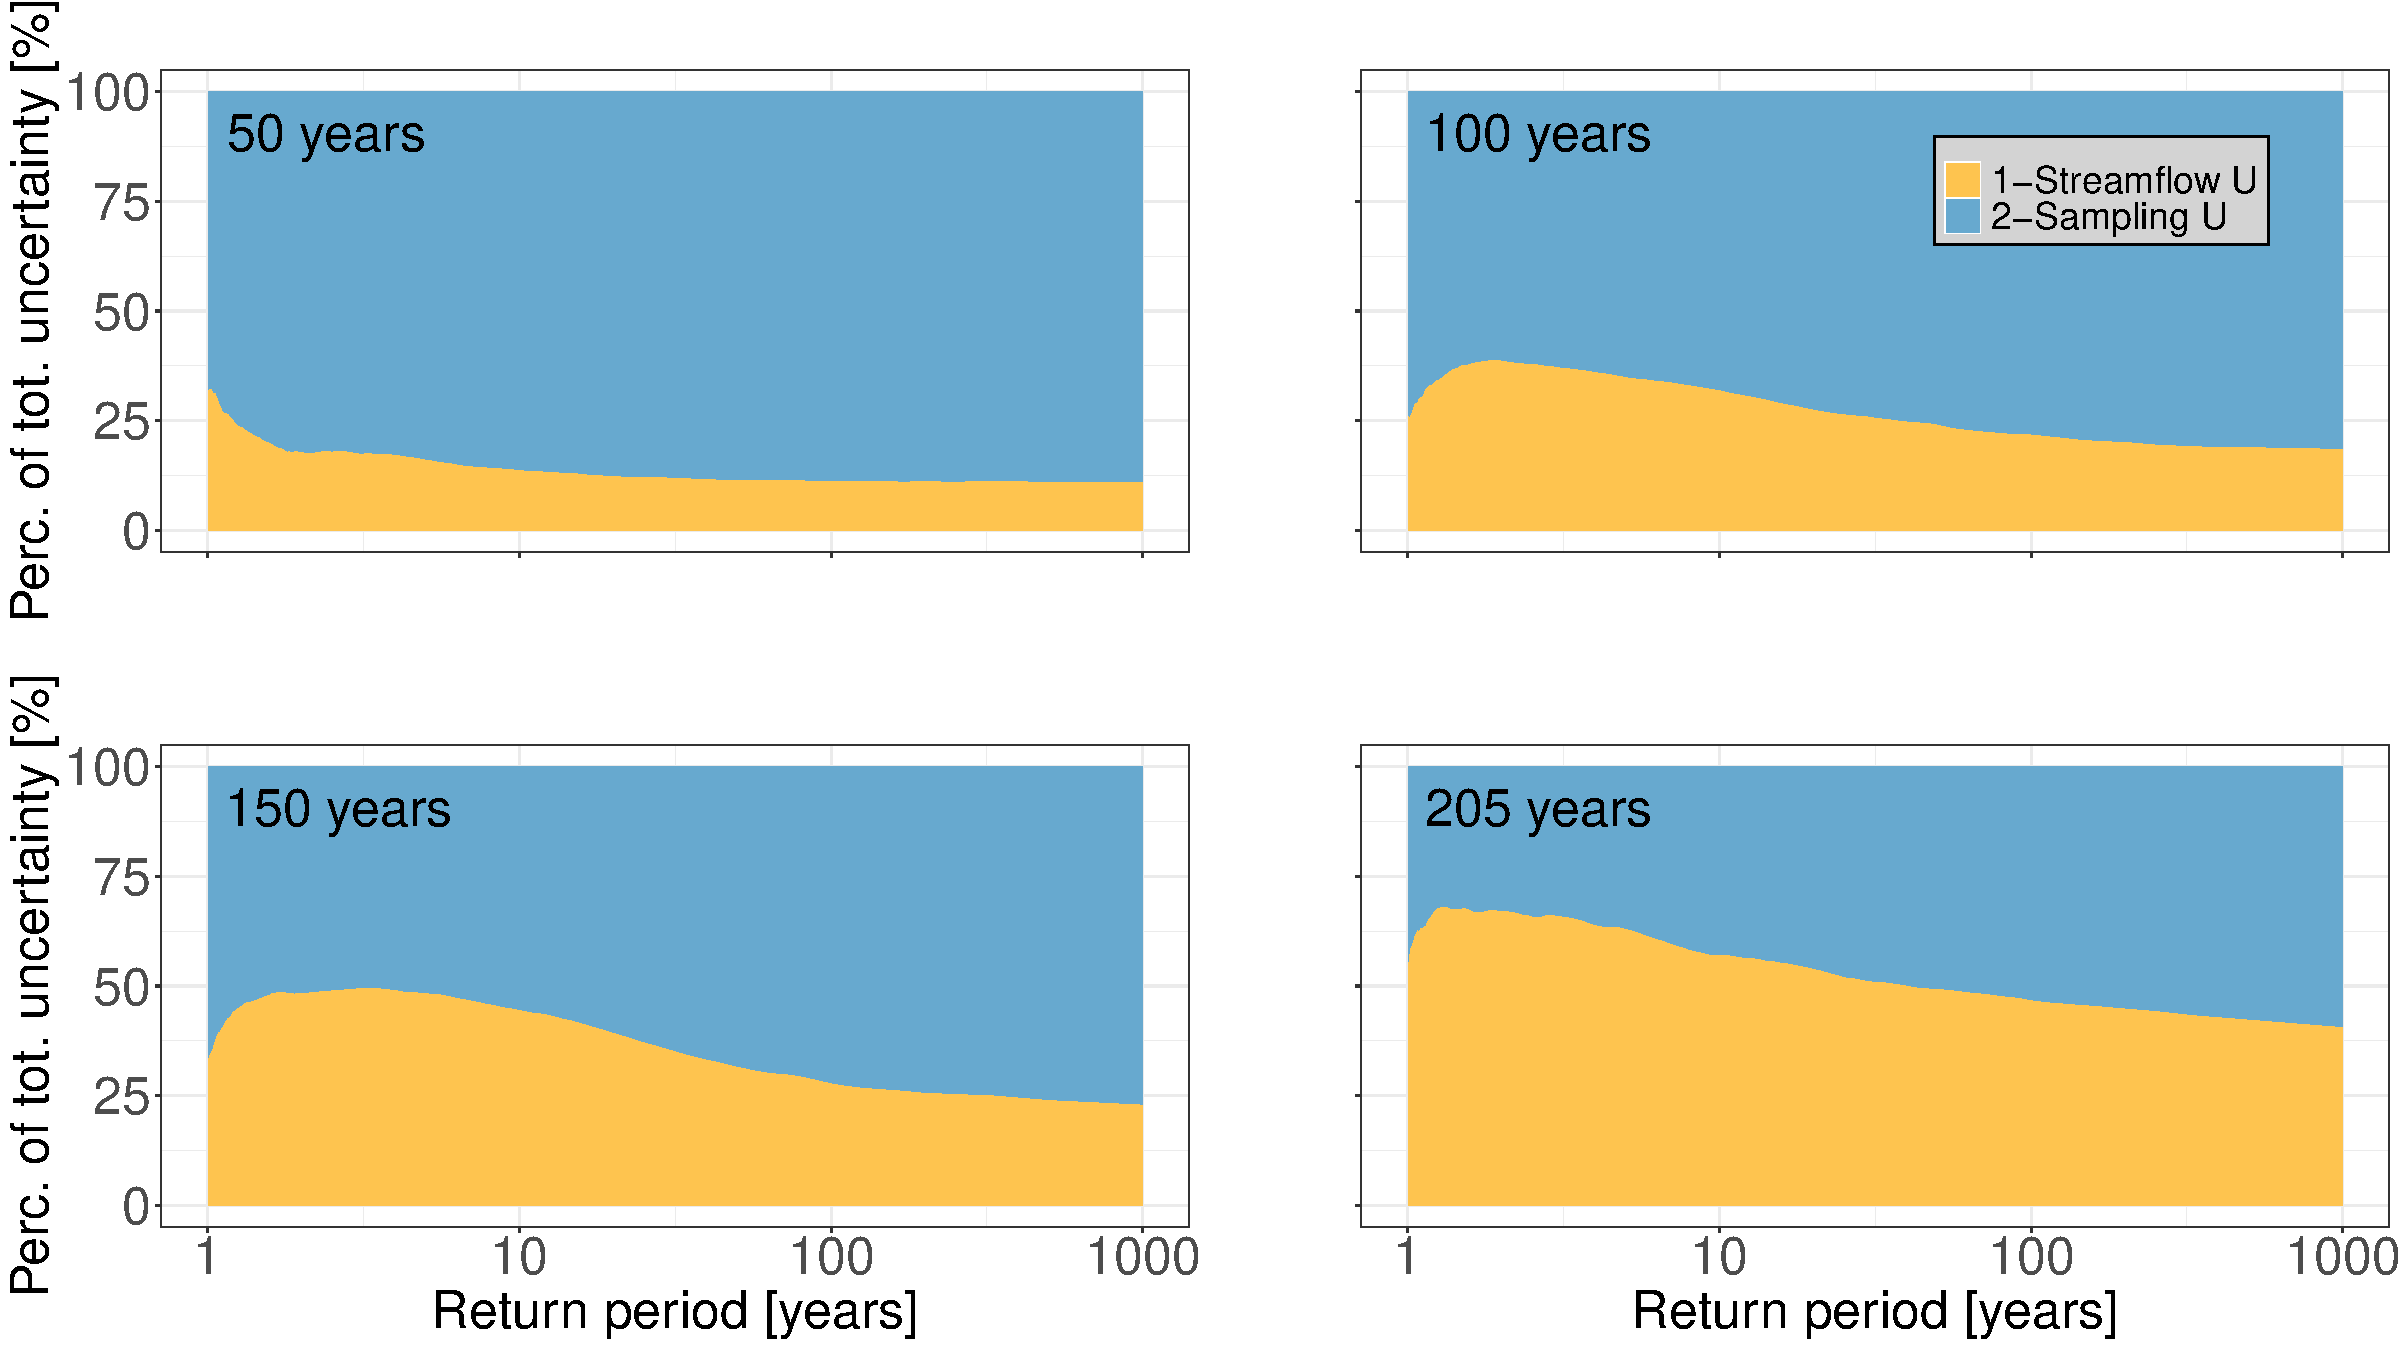
\includegraphics[width=\linewidth]{Chapitre3/Figures/10c-Ukplot4cases.pdf}
                \caption{}
                \label{subfig:UKplot4cases}
            \end{subfigure}
            
            \begin{subfigure}{0.47\textwidth}
                \centering
                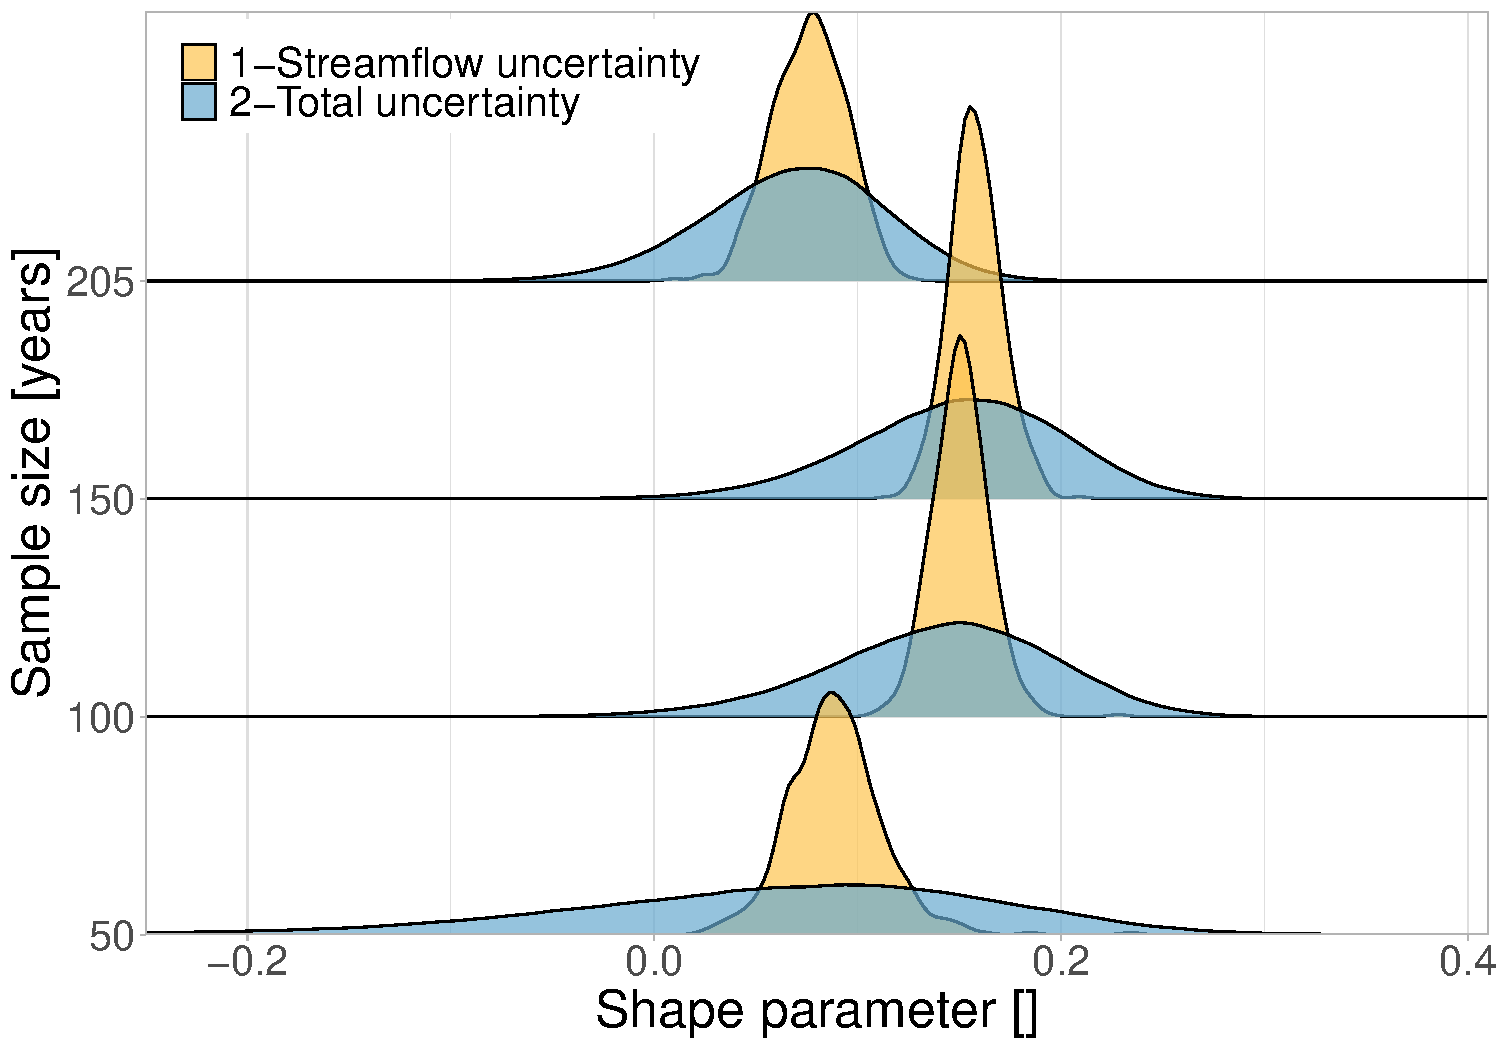
\includegraphics[width=\linewidth]{Chapitre3/Figures/10d-Shape_4cases.pdf}
                \caption{}
                \label{subfig:Shape4cases}
            \end{subfigure}
            \begin{subfigure}{0.52\textwidth}
                \centering
                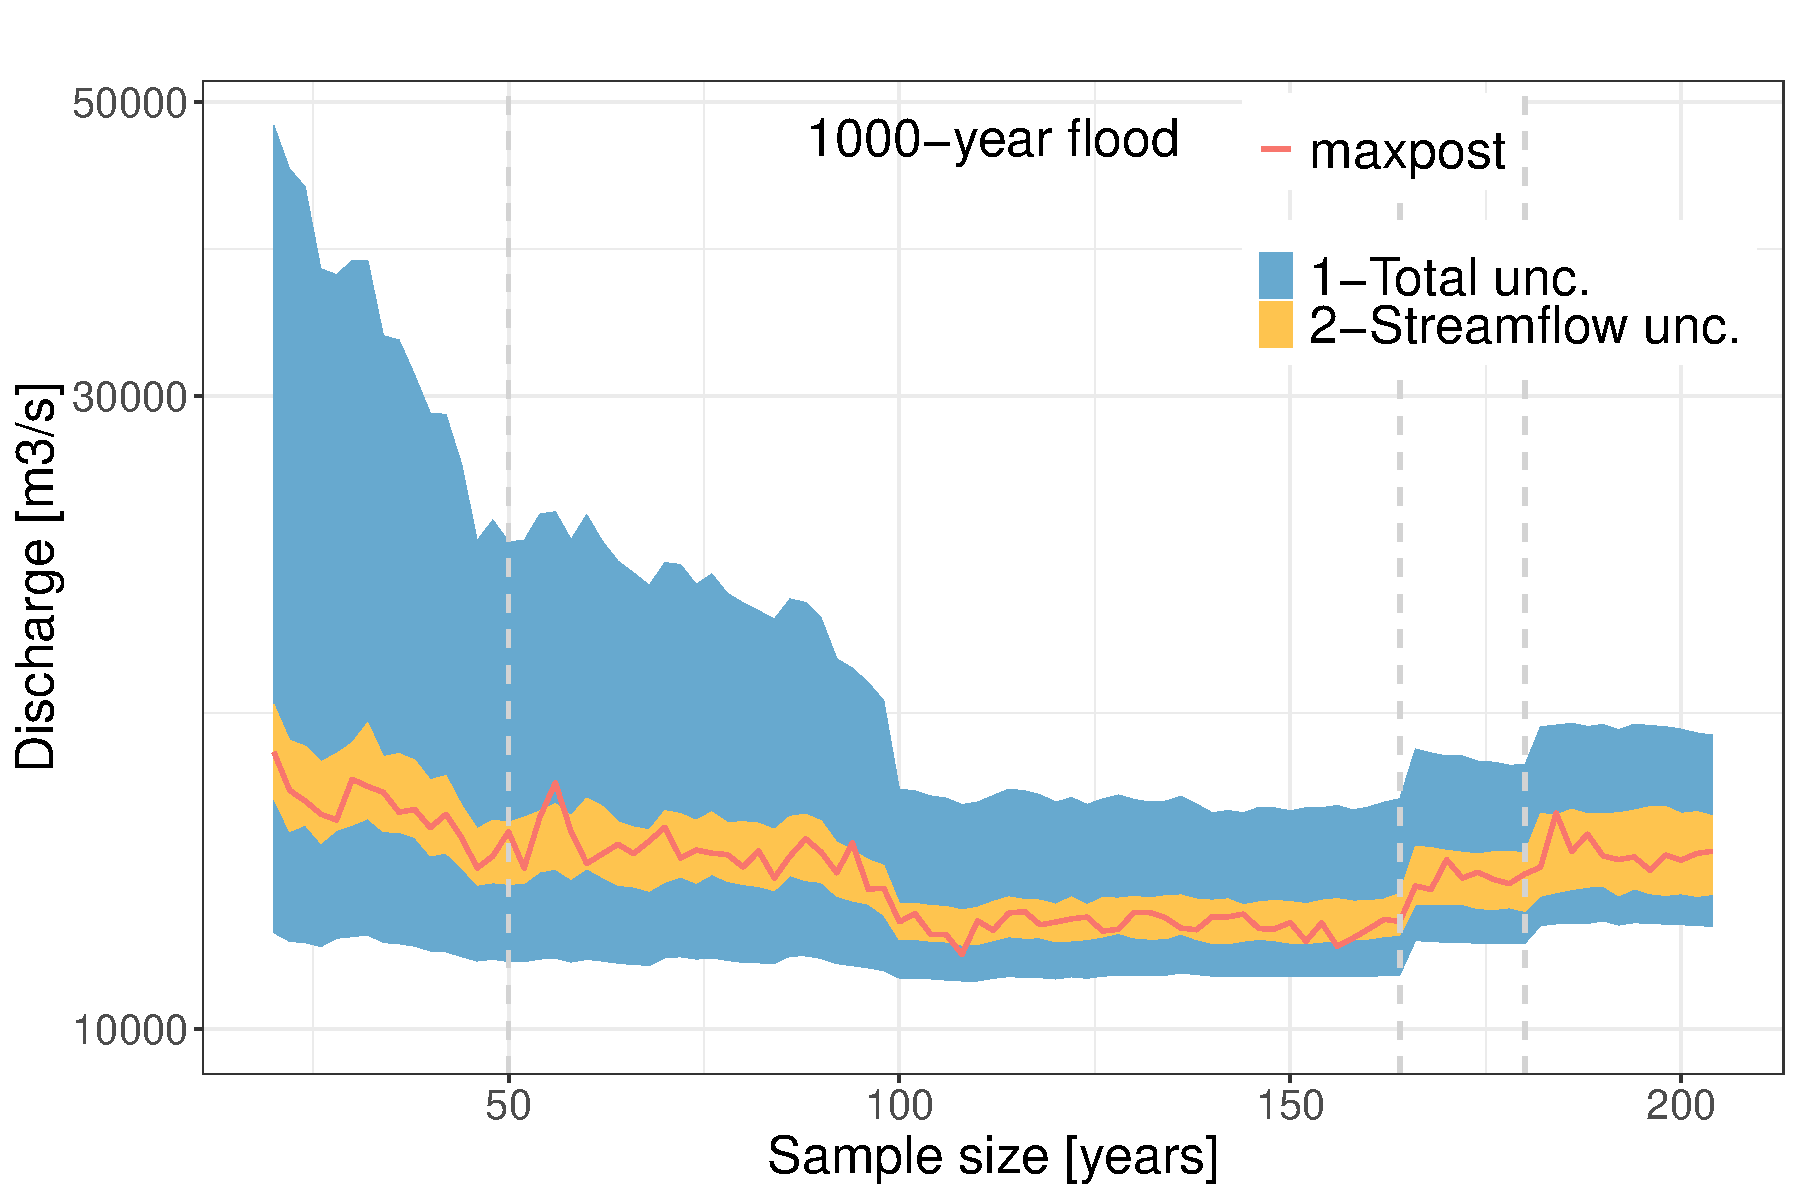
\includegraphics[width=\linewidth]{Chapitre3/Figures/10e-Q1000SSize.pdf}
                \caption{}
                \label{subfig:SamplesQ1000}
            \end{subfigure}
            
            
        \caption{FFA results of the Rhône River at Beaucaire. (a) GEV distribution estimated with the full sample (1816-2020). Error bars represent the observed AMAX discharges with their 95\% streamflow uncertainty.
        (b) Maxpost quantiles estimates for three return periods and four sample sizes. Error bars represent 95\% total uncertainty intervals.
        (c) Contribution of streamflow and sampling uncertainties to the total uncertainty for four sample sizes. 
        (d) GEV shape parameter distributions considering streamflow or total uncertainty for four sample sizes. 
        (e) 1000-year flood estimations for various sample sizes. Grey dotted lines represent large changes in the sample data (the change from Pont de Beaucaire to Beaucaire Restitution gauge en 1967, the inclusion of 1856 flood and the inclusion of 1840 flood to the sample).}
        \label{fig:Quantiles}
        \end{figure}

        \subsubsection{Sample size influence on quantiles uncertainty}
        \label{subsec:SampleSize}
        
        With an exceptionally long sample at Beaucaire, the influence of sample size on flood quantiles estimation in a real case can be quantified, hence assessing the interest of using old hydrometric data when available. Four sample sizes are tested, taken as the last 50 years, 100 years, 150 years, and the largest available sample of 205 years. A figure describing these sub-samples along the AMAX time series is available in supplementary material (figure 3). GEV distributions are estimated and the contribution of both streamflow and sampling uncertainties is computed for each case, following section \ref{subsec:FFA} procedure. Total uncertainty is clearly reduced between the 50 years sample and the other samples for the three return periods: 10, 100 and 1000 years (figure \ref{subfig:BarplotQuantilesGev}). Surprisingly, for the 1000-year flood estimation, the total uncertainty is not reduced between the 100 and 205 years samples. This illustrates that the reduction of sampling uncertainty induced by increasing the sample size may be compensated by the increased streamflow uncertainty when going back in time. Figure \ref{subfig:UKplot4cases} is a good illustration of this phenomenon, showing the augmentation of the relative part of streamflow uncertainty when increasing the sample size.
        
        \paragraph{}
        The maxpost values of the 205 years sample is higher than the 100 and 150 years samples (figure \ref{subfig:BarplotQuantilesGev}), probably because of the inclusion of the two largest floods of the history in the 205 years sample (1840 and 1856 floods). Thus, without using those old hydrometric data (1816-1870), the 1000-year flood could have been 15\% lower in this specific case. Figure \ref{subfig:Shape4cases} shows that the streamflow uncertainty has a minor impact on shape parameter uncertainty compared with the sampling uncertainty. The sample size impact on flood quantiles estimation is further explored in Figure \ref{subfig:SamplesQ1000}. The 1000-year flood (maxpost) and the relative contributions of both sources of uncertainty are estimated for several sample sizes, from 20 to 205 years, with a two-year step. A large reduction of sampling uncertainty (and of the total uncertainty as a consequence) appears between 20 and 100 years, along with the reduction of the maxpost value. Then, the maxpost and uncertainty intervals are constant between 100 and 160 years of sample size, until the inclusion of 1856 and 1840 major floods that lead to a slight increase in the estimated quantile. The total uncertainty interval width is not much changed by those flood inclusions but the relative contribution of streamflow uncertainty is larger.
\FloatBarrier
\section{Discussion}
\label{sec:Discussion}
    \subsection{Usefulness of disentangling the various sources of uncertainty in FFA}

    %cohérence de cette partie
    \paragraph{}
    Even though sampling uncertainty is a major concern in FFA, historical systematic stage records are rarely used. The laborious process of gathering and reanalyzing data, and concerns about the reliability of the resulting discharge series may be the potential reasons for this oversight. Moreover, the estimation and the propagation of the various sources of uncertainty throughout the FFA chain is not straightforward to achieve. Several papers performed an integrated analysis in which both rating curve parameters and flood frequency distribution were estimated (\citet{petersen-overleir_accounting_2009}; \citet{steinbakk_propagation_2016}; \citet{vieira_assessing_2022}). They concluded that accounting for rating curve uncertainties may notably widen the total uncertainty of flood quantiles. More specifically, \citet{steinbakk_propagation_2016} based their case study on several Norwegian rivers, with sample sizes up to 100 years. They found that sampling uncertainty is generally the main contributor (i.e. versus rating curve uncertainty) to design flood estimates and that its contribution decreases when sample size increases.

    \paragraph{}
    The approach proposed in this paper does not only consider rating curve uncertainty, but also stage uncertainties (that combine stage measurement and time interpolation errors) and rating changes. Their consideration is crucial when dealing with long streamflow series. The case study investigated in this paper is based on a 205-year long systematic sample, which enables an in-depth evaluation of the contribution of the different sources of uncertainty in design flood estimates from series of several decades to long series exceeding one century of systematic record. The results show that the estimated 95\% streamflow uncertainty is not negligible and varies from 30\% (XIX\textsuperscript{th} Century) to 5\% (1967-2020). The larger streamflow uncertainty of the XIX\textsuperscript{th} Century is mostly due to stage uncertainty, which emphasises the importance of paying a particular attention to this uncertainty source when using historical stage measurements. Streamflow uncertainty is then propagated to flood quantiles estimates. For the 205-year long flood sample, streamflow uncertainty dominates for return periods below 100 years but sampling uncertainty becomes dominant when the return period tends toward 1000 years. The 205-year long streamflow series enables exploring the contribution of streamflow and sampling uncertainties for various sample sizes. Sampling uncertainty contribution decreases when sample size increases, unlike streamflow uncertainty contribution which increases when older data are included. Although the relative contribution of each source of uncertainty on extreme quantiles varies, the width of the total uncertainty interval does not change much from 100 to 205 years samples. Nevertheless, in this case study, the maxpost value of extreme quantiles is increased by 15\% when considering 205 years rather than 150 or 100 years, as the two largest floods since 1816 occurred during the first 40 years of records. This emphasizes that using longer records does not only affect the uncertainty around flood quantiles, but also the value of the quantiles themselves. 

    % BR: I removed this paragraph, it seems to me that it does not provide any additional information compared with the previous ones.
    %\paragraph{}
    %Unsurprisingly, in this case study, accounting for several sources of streamflow uncertainties in FFA widens the total uncertainty around flood quantiles, as described by \citet{petersen-overleir_accounting_2009}, \citet{steinbakk_propagation_2016} and \citet{vieira_assessing_2022} who only considered rating curve uncertainty. Moreover, similarly to \citet{steinbakk_propagation_2016} who used sample sizes up to 100 years, we found that sampling uncertainty is dominant for samples shorter than 100 years and that sampling uncertainty decreases when sample size increases. However, those two assumptions are not true when increasing the sample size above 100 years at Beaucaire, because sampling uncertainty contribution does not decrease and streamflow uncertainty contribution increases. 
    
    \subsection{Potential improvements of the method and further analyses}
    \paragraph{}
    The streamflow uncertainty analysis procedure proposed in this work is affected by several limitations. The gauging segmentation model proposed by \citet{darienzo_detection_2021} (or more generally any gaugings-based segmentation approach) is limited when gaugings are scarce. Some rating shifts are likely to be missed, and even when one is detected, assigning a precise shift time is difficult when very little information is available about rating changes and channel morphology. Other approaches could be trialed to detect changes in the stage-discharge relationship, such as the analysis of stage or discharge recessions (for instance: \citet{nathan_evaluation_1990}; \citet{tallaksen_review_1995}; \citet{vogel_estimation_1996}; \citet{chapman_comparison_1999}; \citet{lang_extrapolation_2010}; \citet{darienzo_detection_2021-1}) or the occurrences of morphogenic events (\citet{darienzo_detection_2021-1}).    
    \paragraph{}
    Another limitation of the method comes from the elicitation of hydraulic priors in a historical context, for which information about hydraulic configurations is scarce. This lack of knowledge is particularly detrimental for stations where changes in bed morphology are frequent. As described by \citet{petersen-overleir_accounting_2009}, the extrapolation of rating curves in this context is more uncertain, thus affecting flood quantile estimates. 
    \paragraph{}
    The shape parameter is of great importance as it determines the tail behaviour of the GEV distribution. Several regional or local-regional methods have been proposed to reduce the uncertainty of the shape parameter estimation (\citet{burn_evaluation_1990}; \citet{ouarda_regional_2001}; \citet{ribatet_regional_2007}; \citet{micevski_combining_2009}; \citet{haddad_regional_2012}). This could be a source of improvement, but a regional approach could be difficult to apply here, because catchments as large as the Rhône River at Beaucaire cover many different climatic influences and are quite unique, which makes the use of other similar catchments challenging. An alternative solution to this approach is to analyse floods in the main subcatchments and their concomitance.
    \paragraph{}The underlying assumption of stationarity required for FFA is questionnable due to anthropogenic climate change, as described by \citet{milly_stationarity_2008}. However, \citet{madsen_review_2014} underlined that no particular guideline for climate change adjustment factors on design flood are given in France. Trends in flood magnitudes have been identified in several climatic regions of Europe (\citet{hall_understanding_2014}; \citet{bloschl_changing_2019}) and France \citep{giuntoli_floods_2019}, but not everywhere and with large regional differences. Many approaches of FFA accounting for non-stationarity have emerged (as reviewed by \citet{salas_techniques_2018}) and are sometimes combined with regional approaches \citep{han_incorporating_2022}. After identifying the regional trends of the Rhône River, a next challenge could be to develop a climate-informed model to account for the effects of climate change on floods.
    
    \paragraph{}
    Finally, a promising development is to use sporadic flood evidences older than systematic stage measurements. This data can come from various origins such as testimonies \citep{pichard_sept_2014}, flood marks \citep{renard_use_2023}, paleoflood evidences based on slack water deposits \citep{sheffer_paleofloods_2003}, lake sediments \citep{wilhelm_reconstructing_2022} or sediments within the Rhone prodelta \citep{fanget_historical_2013}. Various procedures have been developed in the literature to include such data in FFA through the use of perception threshold and censored data (\cite{brazdil_historical_2006}; \cite{kjeldsen_documentary_2014}; \cite{england_guidelines_2019}; \cite{harden_historical_2021}). Such approaches have been applied in Europe, including France (\citet{naulet_flood_2005}; \citet{lang_extrapolation_2010}; \citet{neppel_flood_2010}; \citet{payrastre_usefulness_2011}) and could be interesting for the Lower-Rhône Valley for which many flood evidences (along with information on other climate-related disasters) have been gathered. \citet{pichard_sept_2014} and \citet{pichard_hydro-climatology_2017} have identified more than 1500 hydro-climatic events in the Lower-Rhône Valley since the XIV\textsuperscript{th} Century, synthesized in the HISTRHÔNE database (\url{histrhone.cerege.fr}). The flood events are classified by magnitude of damages, and further investigations are required to identify the perception thresholds corresponding to those different magnitudes. In addition, as this information is not exhaustive (unlike the stage measurements used in this paper), the extension of the sample before 1816 requires a different statistical treatment. Moreover, the interest of long discharge series and flood evidences is not limited to standard FFA, but is also useful for studying the long-term historical variability of floods (e.g \cite{macdonald_high-magnitude_2017}).
  
    \subsection{Are historical stage records useful for flood frequency analysis?}

    %cette section est un peu courte... tu pourrais replacer le cas de Beaucaire parmi les autres études de la littérature. 
    The interest of including historical stage records to reduce sampling uncertainty in FFA should be balanced against the large streamflow uncertainty induced by those records. For the specific case of Beaucaire, the use of historical stage records is clearly beneficial up to a 100-year sample size, but the added value is not as clear with longer samples (see section \ref{subsec:SampleSize} and figure \ref{fig:Quantiles}). Evaluating the procedure on more stations with historical systematic stage records would be necessary in order to generalize the results. The respective contribution of streamflow and sampling uncertainties could be different for other stations depending on their respective hydraulic configuration and river bed stability.    
    %Aussi, un point important est qu'on peut toujours améliorer (réduire l'incertitude des) débits historiques, en faisant plus d'études historiques, de la géomoprho, de la modélisation hydraulique, etc.  L'exemple du Rhin où Michel dispose de débits modélisés par d'autres est un bon cas (sauf que Michel n'a pas publié l'article...). C'est aussi un cas où l'analyse hydraulique permet de détecter et expliquer une rupture dans les débits : tu peux insister sur l'importance de vérifier l'homogénéité des données.
    \paragraph{}
    In this paper, the estimation of flood discharges follows the usual hydrometric process (i.e. converting the measured stages into discharges via the estimation of rating curves from gaugings). However, the stage measurements and gaugings from the XIX\textsuperscript{th} Century are scarce compared to recent decades, which leads to large uncertainties around flood discharges. Those uncertainties could be reduced in multiple ways, including the use of hydraulic models. This practice is widespread in the literature and is generally applied to floods older than systematic measurements (for instance: \citet{naulet_flood_2005}; \citet{neppel_flood_2010}; \citet{machado_flood_2015}; \citet{ruiz-bellet_uncertainty_2017}; \citet{van_der_meulen_late_2021}). Yet, it requires topographic and bathymetric data that may be even more scarce and uncertain than gaugings. Moreover, the use of flood evidences older than systematic measurements generally leads to the assumption that all the floods greater than an identified perception threshold are known, as well as the magnitude of the threshold itself.
    
    \paragraph{}
    The specific conclusions of the Rhône River at Beaucaire may not be generalized to other climatic regions for which the tail behaviour of flood distribution is influenced by different processes \citep{merz_understanding_2022}. More specifically, the Rhône River at Beaucaire has a positive shape parameter, which corresponds to a right-bounded behavior with the GEV parameterization used in this paper. While this might be typical of such large catchments, many smaller catchments display the opposite heavy-tailed behavior. Whether or not the main conclusions drawn in this paper would still hold with such smaller catchments remains to be evaluated.

    
\section{Conclusion}
\label{sec:Conclusion}

    \paragraph{} Flood hazard estimation is affected by several sources of uncertainty, including sampling uncertainty that is dominant for usual sample sizes (less than 100 years). It is sometimes possible to gather historical systematic stage measurements in order to enlarge flood samples beyond usual sizes. This process has the potential to reduce the uncertainties of design flood estimates. Nevertheless, the streamflow series derived from these historical stage series are generally affected by much greater uncertainties than modern series. This paper investigates the following questions: to what extent does including historical (and thus uncertain) hydrometric data improves FFA estimates, and what is the contribution of streamflow and sampling uncertainties to the total FFA uncertainty ? Those questions are explored through a general FFA framework accounting for the specific uncertainties affecting long hydrometric series. This uncertainty propagation chain is applied to a 205-year long systematic stage series of the Rhône River at Beaucaire.
    \paragraph{} The estimated streamflow uncertainty varies from 30\% (XIX\textsuperscript{th} Century) to 5\% (1967-2020). This uncertainty is propagated to flood quantiles estimates. When using the full flood sample (205 years), streamflow uncertainty is dominant below the 100-year flood and sampling uncertainty is dominant above. However, this conclusion is sensitive to the available sample size. The sample size impact on design flood estimates is explored by subsampling the full flood sample.
    The total uncertainty of flood quantiles substantially decreases from 20- to 100-year samples. This decrease is directly induced by the reduction of sampling uncertainty. For sample sizes between 100 and 205 years, the total uncertainty is nearly constant because the sampling uncertainty reduction is offset by the increase of streamflow uncertainty (older flood discharges are more uncertain). However, the central flood quantiles estimates increase by about 15\% when increasing sample size between 160 and 205 years, because of the inclusion of the two largest floods that occurred during the first 40 years of measurement. Yet, this 15\% increase is slight with respect to the total uncertainty. One should be cautious about generalizing these results beyond the particular case of the Rhône River at Beaucaire, as the contribution of sampling and streamflow uncertainties may strongly depend on the properties of the station and the catchment.
    \paragraph{}
    Finally, this article promotes the use of historical stage records to improve design flood estimates and underline the particular importance of estimating and propagating all sources of uncertainty through the estimation process. Discussions are currently underway with the competent authorities in flood risk management concerning the updating of design flood (Q100, Q1000, Q1500) with enlarged samples (from 80 to 205 year-discharge series), and on ways to account for estimation uncertainty. The use of estimates derived from the predictive distribution (also referred to as the expected probability approach, e.g. \cite{kuczera_comprehensive_1999}; \cite{renard_data-based_2013}) could be considered since it is naturally suited to the Bayesian approach used here. Interesting improvements may come from the use of sporadic flood evidences older than the systematic stage measurements used in this paper, or from regional or non-stationary FFA approaches. Moreover, beyond standard FFA, such long series also have the potential to shed light on the long-term historical variability of floods. 

\section{Acknowledgements}
\paragraph{}
The PhD fellowship of Mathieu Lucas is funded by INRAE, the Compagnie Nationale du Rhône (CNR) and EUR H2O’Lyon (ANR-17-EURE-0018) from the University of Lyon. This study was conducted within the Rhône Sediment Observatory (OSR), a multi-partner research program funded through the Plan Rhône by the European Regional Development Fund (ERDF), Agence de l'eau RMC, CNR, EDF, and three regional councils (Auvergne-Rhône-Alpes, PACA, and Occitanie). Data and expert knowledge on the Rhône River at Beaucaire were provided by CNR, the Rhône Sediment Observatory, Pascal Billy and Helene Decourcelle from the DREAL Auvergne-Rhône-Alpes (Ministry of Ecology) and the HISTRHONE database from the CEREGE (Georges Pichard).
\paragraph{} The data is available at \href{https://www.plan-rhone.fr/publications-131/actualisation-de-lhydrologie-des-crues-du-rhone-1865.html?cHash=5628938abe287dc9ca390dad7373ae0e}{https://www.plan-rhone.fr/} (up to 2016) and uncertainty propagation code with the whole data set ("QuantilesAmax.txt") is available at \url{https://github.com/MatLcs/PropagMaxAn}.

\newpage